\documentclass{article}
\usepackage{graphicx}
\usepackage{booktabs}
\usepackage{tabularx}
\usepackage{amsmath,amssymb}
\usepackage{subcaption}
\usepackage{authblk}
\usepackage[utf8]{inputenc}

\usepackage[colorlinks=true, linkcolor=blue, citecolor=blue, urlcolor=blue]{hyperref}

\newtheorem{definition}{Definition}[section]
\newtheorem{proposition}{Proposition}[section]

\renewcommand\Affilfont{\itshape\footnotesize}

\title{\textbf{Intelligence within Bounds: Why Cognition Requires a Closed Convex Hull}}

\author{Naoki Higuchi}

\affil{CSCT-NAIL (CSCT Neuro-AI Lab), Tokyo, Japan}
\affil{\texttt{contact@csct-nail.com}}
\affil{Code available at: \url{https://github.com/CSCT-NAIL/CSCT}}
\affil{Software DOI: \href{https://doi.org/10.5281/zenodo.18382368}{10.5281/zenodo.18382368}}

\date{\today}

\begin{document}

\maketitle

\begin{abstract}
How do discrete symbolic representations emerge from continuous neural dynamics?
Unlike Bayesian approaches that presuppose prior distributions, we propose Clock-Selected Compression Theory (CSCT), an axiomatic framework grounded in five principles: (1) cognition operates on continuous streams, (2) representations are constrained to convex combinations within a simplex, (3) discrete events emerge via phase-locked clock selection, (4) irreversible anchors impose thermodynamic directionality, and (5) syntax emerges as geometric interpolation within the semantic convex hull rather than symbol concatenation.
Through nine experiments using a minimal neural architecture (the CSCT Engine), we demonstrate that: discretization emerges reliably from continuous dynamics; irreversible anchors outperform self-referential systems in long-term stability; feature binding arises from shared phase without explicit concatenation; semantic grounding requires convex-hull membership (96.7\% vs.\ 16.7\% success for in-hull vs.\ out-hull); and syntactic composition emerges as barycentric interpolation rather than algebraic abstraction.
We identify a phenomenon we term \emph{Ungrounded Symbol Acquisition}---discrete codes assigned without reconstructable meaning---providing a mathematical instantiation of the symbol grounding problem.
These findings suggest that bounded geometric constraints, rather than unbounded scaling, may be necessary for stable, meaningful cognition.
We discuss implications for understanding neural manifolds, the limitations of self-attention architectures, and testable predictions for neurophysiological validation.
\end{abstract}

\section{Introduction}

There is a long history of attempts to mathematically model the human cognitive system. Representative examples in recent years include Bayesian cognitive models \cite{knill2004bayesian, tenenbaum2011grow}, which explain perception and decision-making within a framework of estimating posterior distributions from priors and likelihoods, and Artificial Neural Networks \cite{rumelhart1986learning, lecun2015deep}, which approximate learning via weight updates using backpropagation. These models have achieved high predictive accuracy in specific cognitive tasks.

However, these approaches share a common limitation. While they describe ``what is computed,'' they do not answer the implementation-level question of ``how neural circuits realize that computation.'' In terms of Marr's three levels of analysis \cite{marr1982vision}, they remain at the levels of computational theory and algorithm, leaving the dynamical principles governing the operation of neural circuits unexplained. Furthermore, ``initial condition problems'' remain, such as the origin of prior distributions in Bayesian models and the source of supervisory signals in neural networks.

This study approaches this problem from a different angle. Without presupposing prior knowledge or supervisory signals, we inquire into the minimal dynamical conditions under which a cognitive structure self-organizes from the input signal itself. Specifically, we pose the following question: Under what dynamical constraints do discrete representations emerge and become manipulable in response to external inputs?

This question has been addressed from various perspectives. The free-energy principle \cite{friston2010free} provides a variational framework for self-organizing systems, while attractor networks \cite{hopfield1982neural} demonstrate how discrete stable states can emerge from continuous dynamics. However, neither framework explicitly characterizes the geometric and temporal constraints that govern the continuous-to-discrete transition.

To address this gap, we propose the Clock-Selected Compression Theory (CSCT), an axiomatic framework centered on three core principles: (1) Temporal selection via periodic phase signals (clocks), (2) Compressive encoding from continuous inputs to discrete symbols, and (3) Combinatorial operations between discrete representations. CSCT builds on the foundations of free-energy minimization and attractor dynamics by explicitly characterizing the \emph{geometric constraints} (convex hull) and \emph{temporal structure} (phase-locked clocks) that govern symbol emergence. These principles are formulated as five axioms, deriving predictions verifiable through numerical simulation.

The structure of this paper is as follows: Section 2 defines the five axioms of CSCT. Section 3 explains the CSCT Engine, which serves as the foundation for computational experiments, and Section 4 and subsequent sections report on verification experiments for each axiom.

\section{The 5 Axioms of CSCT}

\subsection*{Axiom 1: Streams}
Cognition operates on continuous, time-indexed streams. Agents receive and transmit these signals without assigning privileged status to any specific sensory modality.

\subsection*{Axiom 2: Constructive Compression in Simplex}
Signal approximation is performed via non-negative convex combinations of basis vectors within a Hilbert space. This restricts the latent state to a \textbf{Simplex} (Convex Hull), enforcing constructive compositionality over subtractive interference.

\subsection*{Axiom 3: Multi-Clock Factorization}
Internal inference is performed relative to discretely selected phase signals (clocks) $\tau$. Distinct tasks or contexts induce distinct effective clocks, factorizing the continuous stream into discrete cognitive events.
We use \emph{inference} to denote the evolution of internal states (gate selections and latent variables) with fixed parameters.
In contrast, \emph{learning} refers to parameter updates that change weights and/or the codebook.

\subsection*{Axiom 4: Irreversible Anchor as Command}
An anchoring process $y(t)$ exists as a driving force for state evolution. This signal functions as a command that imposes thermodynamic irreversibility, strictly prohibiting the rewinding of internal time states.

\subsection*{Axiom 5: Barycentric Syntax (Geometric Interpolation)}
Syntax is defined not as abstract symbolic manipulation, but as geometric interpolation within the semantic convex hull.
A novel composite state $S_{\text{composite}}$ is inferable if and only if it can be represented as a convex combination of existing primitive codes $\{C_k\}$:
\begin{equation}
    S_{\text{composite}} \approx \sum_{k=1}^{K} \lambda_k C_k, \quad \text{subject to } \sum_k \lambda_k = 1, \quad \lambda_k \ge 0.
\end{equation}
This axiom restricts constructive inference to the interior of the simplex spanned by the codebook (interpolation), prohibiting unbounded extrapolation outside the hull.

\begin{table}[h]
    \centering
    \caption{Cognitive roles of the CSCT Axioms}
    \label{tab:axiom_roles} 
    \begin{tabular}{@{}ll@{}} 
        \toprule
        \textbf{Axiom} & \textbf{Role in Cognition} \\
        \midrule
        A1 & Guarantees generality of input \\
        A2 & Driving force of representation formation \\
        A3 & Mathematical definition of attention  \\
        A4 & Stabilization of processing \\
        A5 & Geometric basis of syntax\\
        \bottomrule
    \end{tabular}
\end{table}

\section{Computational Experiment Platform: CSCT Engine}

\begin{figure}[htbp]
    \centering
    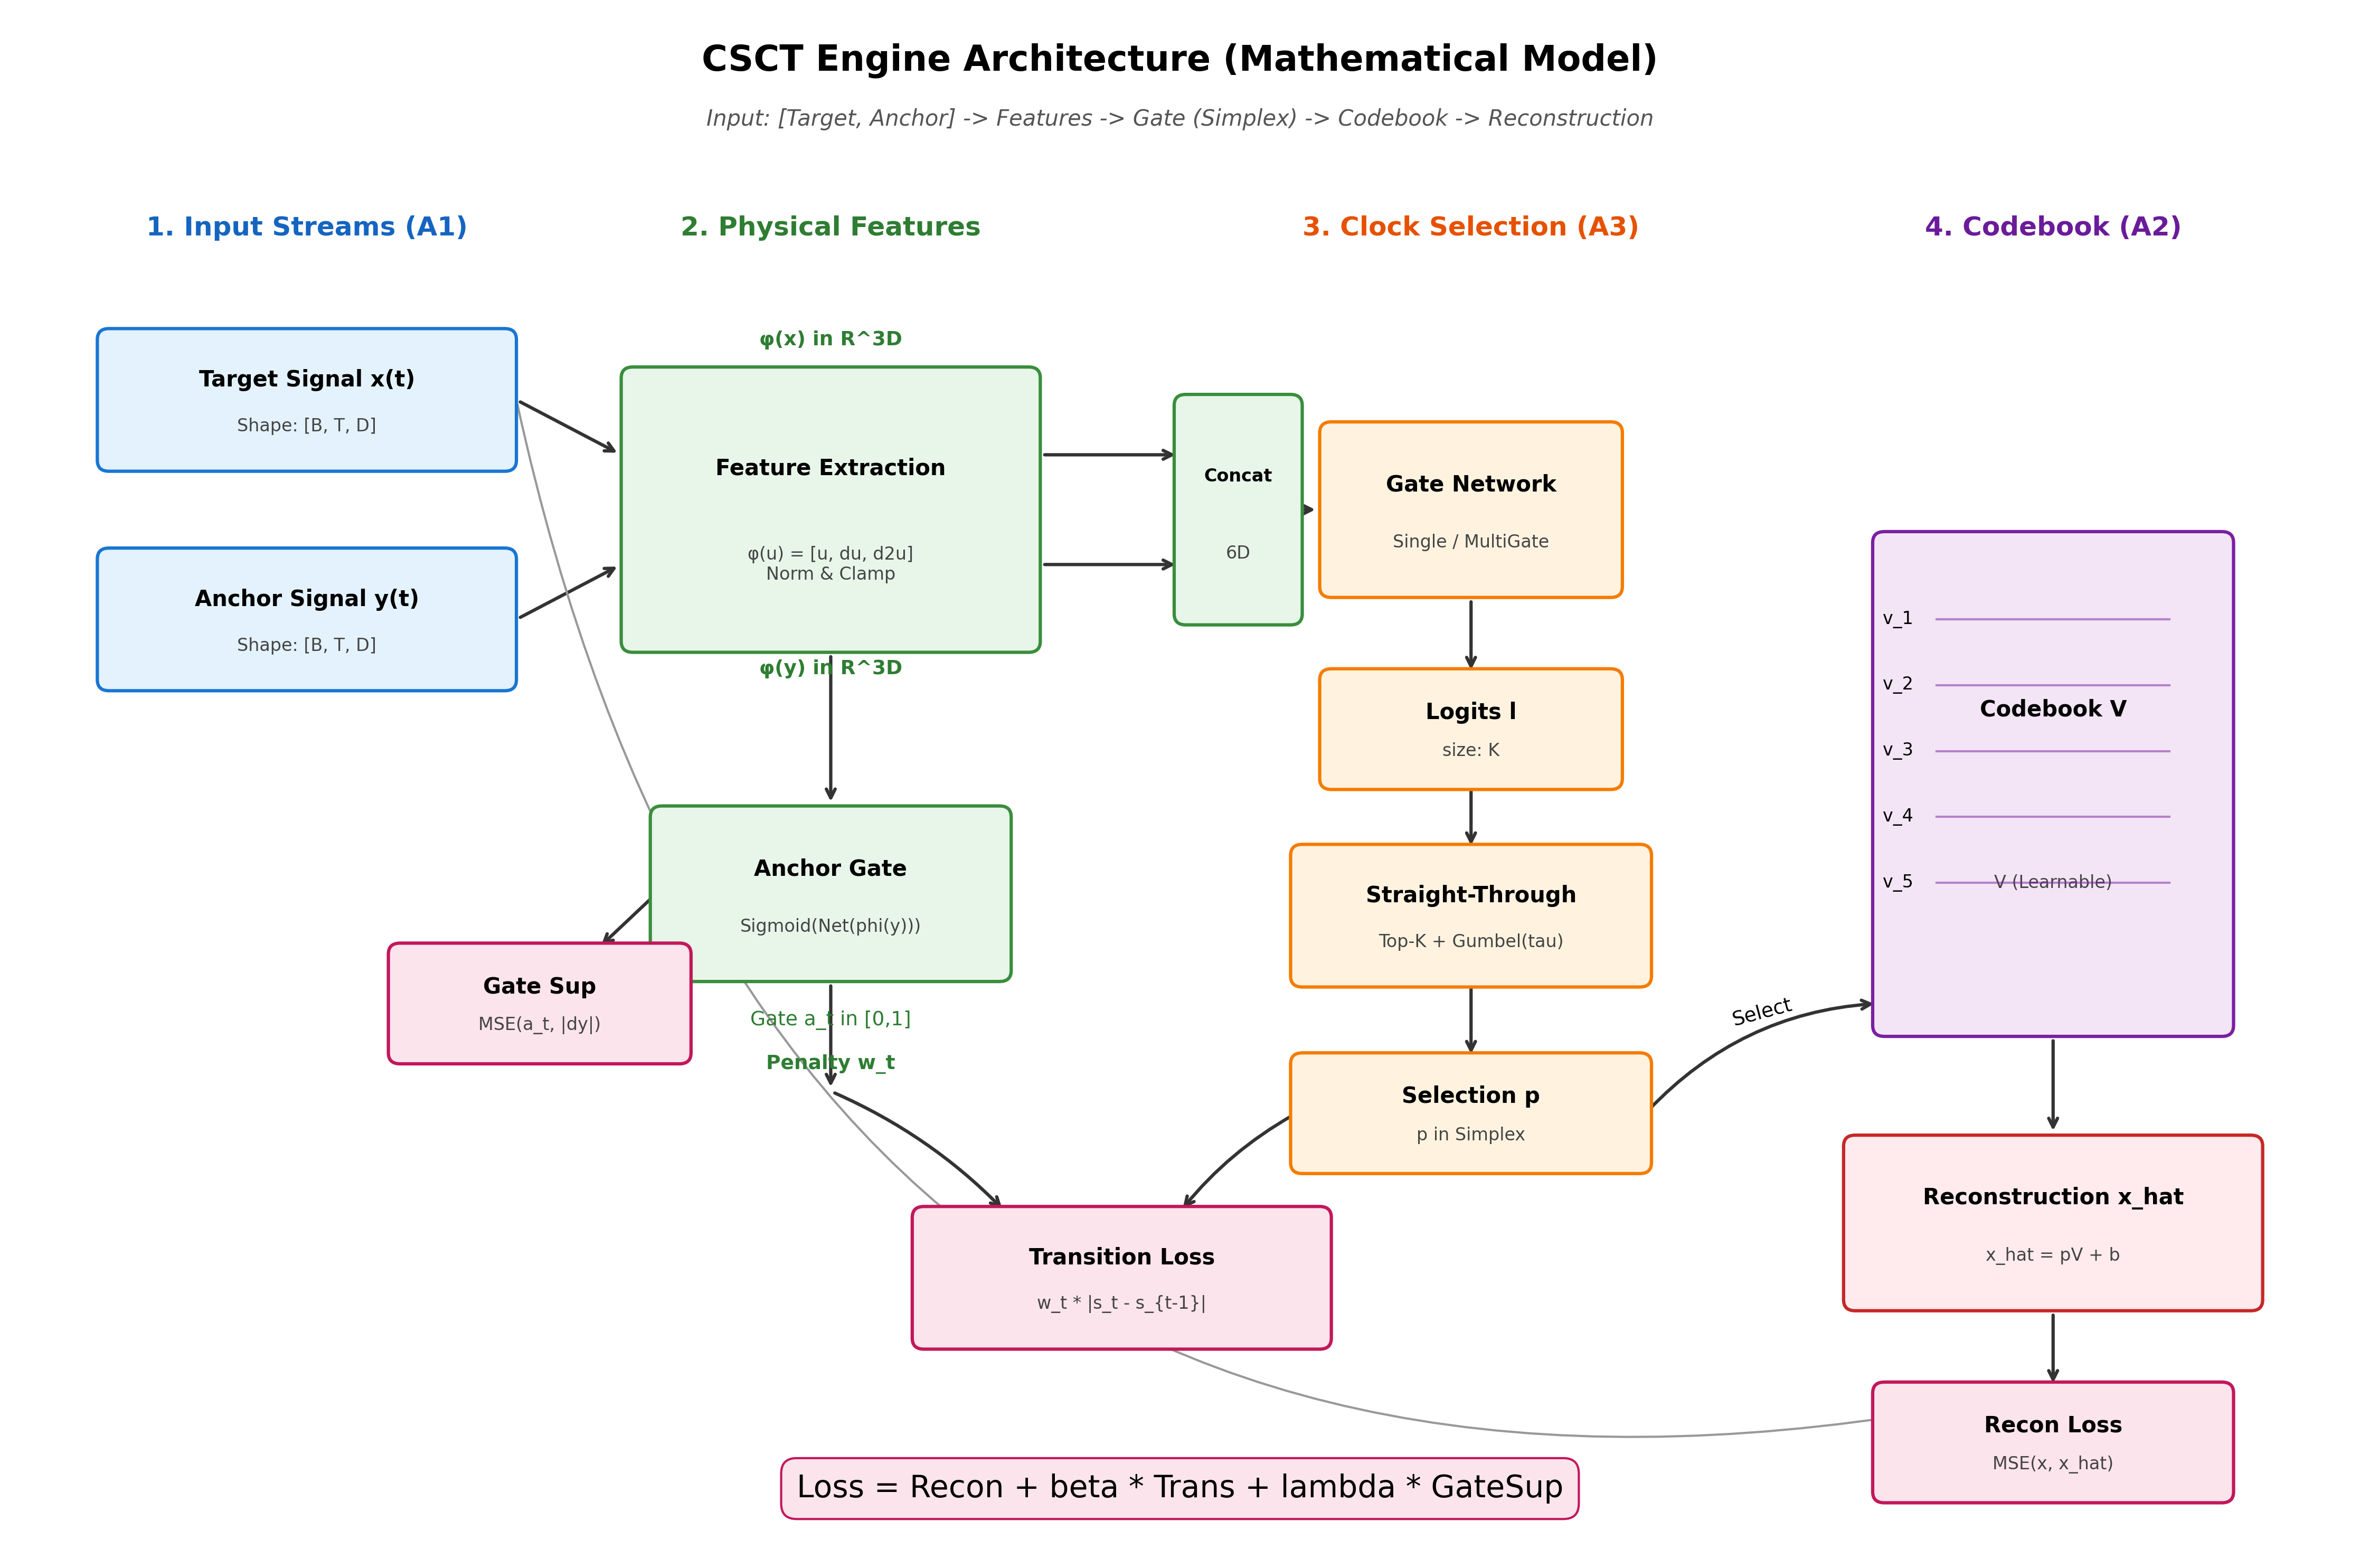
\includegraphics[width=\linewidth]{csct_arch.png}
    \caption{\textbf{Overview of the CSCT Engine Architecture.} The model integrates physical feature extraction, simplex-constrained clock selection, and anchor-modulated transition dynamics to ensure geometric grounding.}
    \label{fig:csct_architecture}
\end{figure}


\subsection{Design Philosophy}
The CSCT Engine is a neurodynamical simulator that implements the 5 axioms in a computable format. It is constructed as a module capable of learning via gradient descent, modeling the process by which various operations emerge from continuous time-series input.

This engine mathematically models cognition as a \textbf{Projected Dynamical System (PDS)} evolving on a Simplex. Unlike standard deep learning approaches that operate in unconstrained vector spaces allowing negative weights (subtractive interference), the CSCT Engine enforces a non-negative constraint ($\mathcal{C} \ge 0$) with unit sum ($\sum_k p_k = 1$). This ensures that the system cannot "rewind" entropy via mathematical cancellation, but must "construct" meanings within the \textbf{Simplex} defined by the codebook vectors, thereby grounding the internal symbols in physical causality.

This engine verifies axioms A1–A5 through the reconstruction and discretization of time-series signals. This section explains the core architectures and the specific implementation of the anchor mechanism.

\subsection{Single-Gate Architecture}
The Single-Gate architecture is defined to possess a single attentional focus. For multi-dimensional inputs, it applies a \emph{winner-take-all Top-1 routing mechanism} to select the most salient channel at each timestep, processing only that channel via the clock selection mechanism. Therefore, SingleGate should be interpreted as a \emph{single-channel view per timestep} rather than a clock shared across all channels.

\noindent\textbf{Implication.} The primary limitation of SingleGate in relational tasks is not ``shared timing across channels,'' but the loss of simultaneous conditioning on multiple channels (i.e., relational information is discarded when only one channel is routed at each timestep).

\paragraph{Processing Flow:}
\begin{enumerate}
    \item \textbf{Feature Extraction:} Extract features $[y, dy/dt, d^2y/dt^2]$ from input signal $x(t)$ and anchor signal $y(t)$.
    \item \textbf{Clock Selection (A3):} Calculate clock selection logits from feature vectors.
    \item \textbf{Discretization (A2):} Discrete selection of the clock via Straight-Through Top-K.
    \item \textbf{Reconstruction:} Reconstruct the signal using the codebook vector corresponding to the selected clock.
    \item \textbf{Anchor Gate (A4):} Adjust transition penalties according to the anchor phase.
\end{enumerate}

\paragraph{Features:}
\begin{itemize}
    \item Suitable for processing single-source waveforms (single channel).
    \item Low computational cost and stable learning.
    \item Due to independent processing of each channel, there are limits to encoding inter-channel relationships.
\end{itemize}

\subsection{Multi-Gate Architecture}
The Multi-Gate architecture possesses multiple gate mechanisms inspired by biological neural mechanisms. It corresponds to central processing.

\paragraph{Three Gate Mechanisms:}

\begin{table}[h]
    \centering
    \caption{Gate mechanisms in the Multi-Gate Architecture}
    \small
    \resizebox{\columnwidth}{!}{%
    \begin{tabular}{@{}lll@{}}
        \toprule
        \textbf{Gate} & \textbf{Biological Correspondence} & \textbf{Role} \\
        \midrule
        Na$^+$ Gate & Sodium channels & High-speed, sparse clock selection \\
        $\theta$ Phase & Hippocampal $\theta$ rhythm & Time-dependent rhythm modulation \\
        NMDA Gate & NMDA receptors & Phase-dependent integration window \\
        \bottomrule
    \end{tabular}
    } %
\end{table}

\paragraph{Features:}
\begin{itemize}
    \item Capable of encoding relational information between channels.
    \item Realizes hierarchical temporal structures similar to $\theta-\gamma$ coupling.
    \item Suitable for integrated processing of multi-channel inputs.
\end{itemize}

\begin{table}[h]
    \centering
    \caption{Comparison of Architectures}
    \small
    \resizebox{\columnwidth}{!}{%
    \begin{tabular}{@{}lll@{}}
        \toprule
        \textbf{Perspective} & \textbf{Single-Gate} & \textbf{Multi-Gate} \\
        \midrule
        \textbf{Biological Correspondence} & Peripheral Processing & Central Processing \\
        \textbf{Channel Processing} & Top-1 channel routing / single clock & Joint multi-channel integration \\
        \textbf{Computational Cost} & Low & High \\
        \textbf{Application} & Single Source Waveform & Inter-channel Relationships \\
        \bottomrule
    \end{tabular}
    } %
\end{table}

\subsection{Anchor Gate Mechanism}
To satisfy A4 (Irreversible Anchor), the engine implements an explicit anchor gate mechanism distinct from the feature extraction modules. This mechanism ensures that internal cognitive time is grounded in the physical time of the environment.

\paragraph{Mechanism:}
The anchor gate network receives the physical feature vector of the anchor signal $y(t)$ (position, velocity, acceleration) and computes a scalar gate activation $a_t \in [0, 1]$ via a sigmoid function. This activation dynamically modulates the transition penalty weight $w_t$ in the objective function:

\begin{equation}
    w_t = w_{floor} + (1 - a_t)(1 - w_{floor})
    \label{eq:anchor_weight}
\end{equation}

When the anchor is static ($a_t \approx 0$), the penalty $w_t$ is maximized, inhibiting internal state transitions. Conversely, when the anchor changes ($a_t \approx 1$), the penalty decreases, allowing the system to update its internal representation.

\paragraph{Synchronization:}
Furthermore, the anchor gate is supervised to synchronize with the magnitude of the anchor's velocity $|\dot{y}|$. This imposes a constraint where the "window of cognition" opens only when there is physical change in the reference frame, mathematically preventing the rewinding of internal time against the environmental anchor.

In discrete time, we approximate the anchor velocity magnitude using channel-averaged L1 norm:
\begin{equation}
v_t := \frac{1}{D}\sum_{d=1}^{D} |y_{t,d} - y_{t-1,d}|,
\qquad
\tilde{v}_t := \frac{v_t}{\max_{t} v_t + \varepsilon},
\label{eq:anchor_velocity}
\end{equation}
and supervise the scalar gate activation $a_t$ to match $\tilde{v}_t$.

\paragraph{Note on multi-channel anchors.}
In the general case $y_t\in\mathbb{R}^D$, we define $v_t$ using the channel-averaged L1 norm as above for gate supervision. However, the anchor gate network itself receives features $\phi(y_t)\in\mathbb{R}^{3}$ computed from a \emph{representative channel} (by default, the first channel $y_{t,1}$). This design choice reduces computational complexity while preserving the essential temporal dynamics of the anchor signal. The supervision target $\tilde{v}_t$ aggregates information across all channels, ensuring the gate learns to respond to overall anchor movement even though its input features come from a single representative channel. In Experiment~1, we use a single-channel self-referential anchor ($y=x$), hence $\phi(y_t)\in\mathbb{R}^{3}$.

\subsection{Learning Objective Function}
The reconstruction $\hat{x}_t$ is defined as an affine combination within the Simplex of codebook vectors $V \in \mathbb{R}^{K \times D}$ plus a learnable bias $b \in \mathbb{R}^D$:
\begin{equation}
    \hat{x}_t = \sum_{k=1}^{K} p_{t,k} V_k + b, \quad \text{s.t.} \quad p_{t,k} \ge 0, \quad \sum_{k} p_{t,k} = 1
    \label{eq:reconstruction}
\end{equation}
where $p_t$ is the sparse activation vector generated by the gate mechanism (typically a one-hot or top-k sparse vector in the discretization limit). The loss function is defined as:
\begin{equation}
\mathcal{L}
=
\mathrm{MSE}(x,\hat{x})
+
\beta \cdot \mathbb{E}_{b,t}\!\left[\mathbb{I}[s_{b,t}\neq s_{b,t-1}] \, w_{b,t}\right]
+
\lambda_g \cdot \mathrm{MSE}(a,\tilde{v}),
\label{eq:loss_function}
\end{equation}
where $\mathbb{E}_{b,t}$ denotes averaging over batch and time, $w_t$ is defined in Eq.~\eqref{eq:anchor_weight}, $\tilde{v}_t$ is the normalized anchor-velocity magnitude defined in Eq.~\eqref{eq:anchor_velocity}, and $\beta$ is the transition penalty coefficient (see Section~\ref{sec:impl_details} for its training schedule).

\begin{itemize}
    \item \textbf{Reconstruction Loss:} Faithful restoration of the signal (A2).
    \item \textbf{Transition Penalty:} Suppression of transitions weighted by the anchor gate $w_t$ (A4).
    \item \textbf{Gate Supervision Loss:} Synchronization of normalized anchor velocity $\tilde{v}_t$ and gate opening $a_t$.
\end{itemize}

\subsection{Implementation Details}
\label{sec:impl_details}

For reproducibility, we specify the following implementation details of the CSCT Engine:

\paragraph{Feature Normalization.}
Physical features $[y, dy/dt, d^2y/dt^2]$ are normalized by dividing by twice the standard deviation computed across the batch and time dimensions, then clamped to $[-3, 3]$:
\begin{equation}
    \phi_{\text{norm}}(f) = \text{clamp}\left(\frac{f}{2 \cdot \text{std}(f) + \varepsilon}, -3, 3\right)
\end{equation}

\paragraph{Discrete Selection with Gumbel Noise.}
Clock selection uses the Straight-Through Top-K estimator with optional Gumbel noise for exploration during training:
\begin{equation}
    \tilde{\ell}_k = \ell_k + \sigma_g \cdot G_k, \quad G_k \sim \text{Gumbel}(0,1)
\end{equation}
where $\sigma_g$ is the Gumbel noise scale (default: 0.5).

\paragraph{Temperature Annealing.}
To achieve gradual discretization, a temperature parameter $T$ is annealed during training:
\begin{equation}
    T^{(e+1)} = \max(T^{(e)} \cdot \gamma, T_{\min})
\end{equation}
where $e$ denotes the epoch, $\gamma = 0.995$ is the annealing rate, and $T_{\min} = 0.1$ is the minimum temperature. The effective softmax temperature is $T_{\text{eff}} = T_{\text{base}} \cdot T$.

\paragraph{Codebook Initialization.}
The codebook vectors are initialized from a Gaussian distribution:
\begin{equation}
    V_k \sim \mathcal{N}(0, 0.5^2), \quad b = 0
\end{equation}

\paragraph{Transition Penalty Coefficient $\beta$.}
The coefficient $\beta$ in Eq.~\eqref{eq:loss_function} follows a two-phase schedule:
\begin{enumerate}
    \item \textbf{Warmup Phase} (epochs $1$ to $E_w$, default $E_w=250$): $\beta$ linearly increases from 0 to a target value $\beta_{\text{target}}$, allowing the codebook to stabilize before enforcing strong discretization:
    \begin{equation}
        \beta^{(e)} = \frac{e}{E_w} \cdot \beta_{\text{target}}, \quad e \le E_w
    \end{equation}
    \item \textbf{Main Phase} (epochs $> E_w$): $\beta$ becomes a learnable parameter via $\log \beta$ parameterization, clamped to $[-5, 5]$ for numerical stability. This allows the model to adaptively balance reconstruction accuracy against transition sparsity.
\end{enumerate}

\clearpage

%%%%%%%%%%%%%%%%%%%%%%%%%%%%%%%%%%%%%%%%%%%%%%%%%%%%%%%%%%%%%%%%%
% EXPERIMENT 1: Single-Channel Waveform Discretization
%%%%%%%%%%%%%%%%%%%%%%%%%%%%%%%%%%%%%%%%%%%%%%%%%%%%%%%%%%%%%%%%%
\section{Experiment 1: Single-Channel Waveform Discretization}

\subsection{Purpose}
Experiment 1 (EX1) examines the fundamental discretization capability of CSCT at the peripheral processing level. This experiment tests whether SingleGate architecture can achieve stable discrete quantization of single-channel waveforms without requiring complex relational processing.

\subsection{Task Design}
The task is to discretize a single continuous waveform into a sequence of discrete codes while minimizing reconstruction error. This represents the most basic form of signal processing in CSCT: converting continuous analog input into discrete symbolic representation.

We use nine waveform types to ensure that the discretization capability generalizes across diverse signal characteristics:
\begin{itemize}
    \item \textbf{sine}: Pure sinusoid. Tests basic periodic discretization.
    \item \textbf{chirp}: Frequency sweep from low to high frequency. Tests adaptation to time-varying frequency.
    \item \textbf{am}: Amplitude-modulated signal. Tests response to envelope dynamics.
    \item \textbf{fm}: Frequency-modulated signal. Tests response to instantaneous frequency changes.
    \item \textbf{ecg}: ECG-like waveform with periodic sharp peaks. Tests handling of transient events.
    \item \textbf{saw\_bl}: Band-limited sawtooth. Tests response to asymmetric waveforms.
    \item \textbf{composite}: Sum of multiple frequency components. Tests multi-scale representation.
    \item \textbf{noisy}: Sine wave corrupted by Gaussian noise. Tests noise robustness.
    \item \textbf{burst}: Intermittent signal with silent periods. Tests handling of onset/offset.
\end{itemize}

The model receives the waveform as input and must learn a codebook of $K$ discrete codes. At each time step, the model selects one code via $\arg\max$ and reconstructs the signal from this discrete representation. Two architectures are compared: SingleGate (shared clock for all dimensions) and MultiGate (independent clocks per channel).

\subsection{Hypothesis}
EX1 tests the fundamental prediction that minimal architecture suffices for single-channel discretization:

\begin{itemize}
    \item \textbf{H1 (SingleGate Sufficiency):} For single-channel waveforms with self-referential anchoring, SingleGate architecture will achieve low reconstruction error. The rationale is that when there is only one information source, a shared clock mechanism can track the signal dynamics without needing to coordinate between channels.
    
    \item \textbf{H2 (MultiGate Redundancy):} MultiGate architecture will perform \textit{worse} than SingleGate on this task, despite having greater representational capacity. The rationale is that MultiGate's independent gating mechanism is designed for relational processing between channels; without multiple channels to relate, this additional complexity becomes a liability rather than an asset, introducing unnecessary degrees of freedom that destabilize learning.
    
    \item \textbf{H3 (Waveform Generalization):} The performance advantage of SingleGate will hold across diverse waveform types (periodic, aperiodic, noisy, transient), indicating that the architectural distinction is fundamental rather than task-specific.
\end{itemize}

If H1--H3 are supported, this would suggest that CSCT correctly predicts a functional dissociation: simpler architecture for simpler (single-source) tasks, with complexity reserved for relational processing.

\subsection{Method}
In peripheral sensory processing, the system operates without access to external reference signals. We employ a self-referential anchor configuration where the anchor signal $y$ equals the input signal $x$ ($y=x$). This represents the simplest form of anchoring in CSCT: the signal serves as its own temporal reference.

\subsubsection{Anchor Configuration}
Self-referential anchor configuration: $y = x$. The input signal serves as its own anchor.

\subsubsection{Parameters and Training}
\begin{itemize}
    \item \textbf{Model Parameters:} Codebook size $K=8$, transition penalty $\beta_{\mathrm{target}}=50$.
    \item \textbf{Training Configuration:} Sequence length $T=200$, total steps $S=500$, $N=20$ seeds per condition. Transition penalty $\beta$ is linearly warmed up from $0$ to $\beta_{\mathrm{target}}$ during the first 200 steps.
\end{itemize}

\subsection{Metrics}
\begin{itemize}
    \item \textbf{Reconstruction Loss (MSE):}
    \begin{equation}
        \mathcal{L}_{\text{recon}} = \|x - \hat{x}\|^2
    \end{equation}
    \item \textbf{Transition Rate:} Fraction of time steps where the discrete code changes.
    \item \textbf{Unique Codes Used:} Number of distinct codes activated during processing.
    \item \textbf{Code Entropy (Normalized):} Entropy of the code distribution normalized by $\log K$.
\end{itemize}

\subsection{Results}
We evaluate EX1 across 9 single-channel waveform types and 20 random seeds (180 paired wave$\times$seed trials), using the self-anchor setting $y(t)=x(t)$.
Figure~\ref{fig:ex1_aggregate} provides a qualitative comparison, and Table~\ref{tab:ex1} reports per-waveform means ($\pm$ std across seeds) for both architectures.

\begin{figure}[t]
    \centering
    % Generated by plot_ex1_comparison.py
    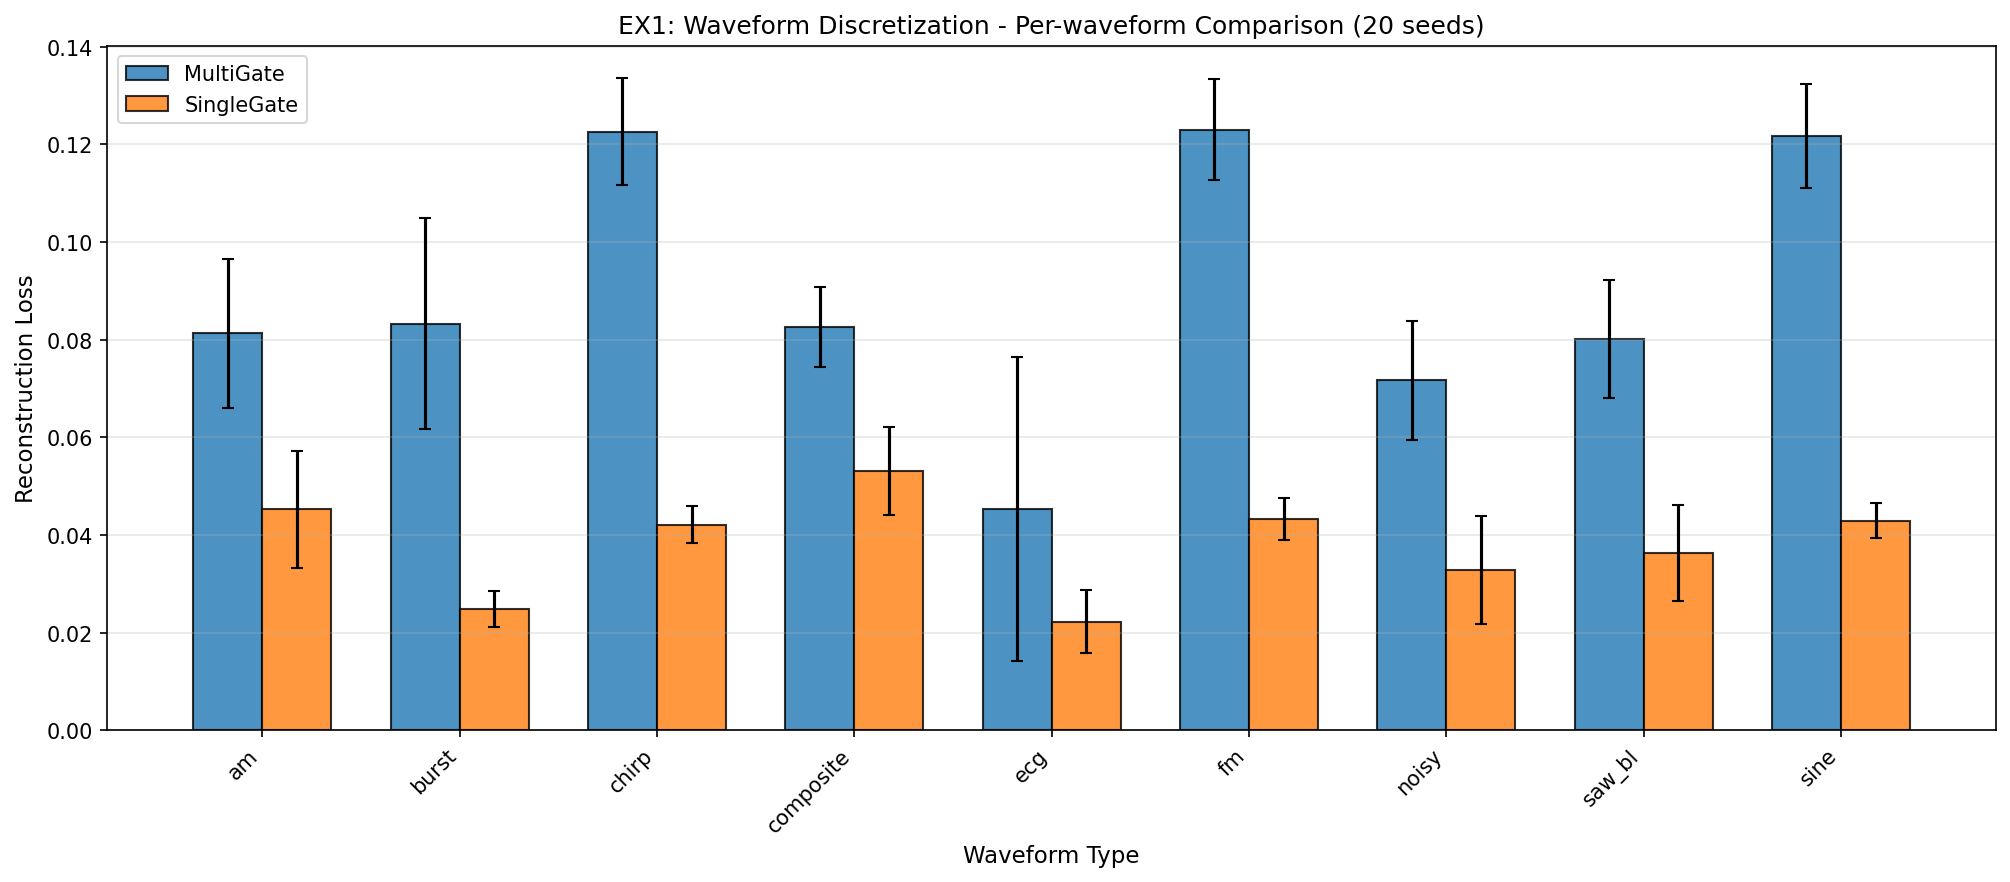
\includegraphics[width=1.0\textwidth]{results_ex1/ex1_aggregate.png}
    \caption{\textbf{Architecture comparison on single-channel waveform discretization (self-anchor).}
    SingleGate yields stable discretization with low reconstruction loss.
    MultiGate also forms discrete states but exhibits consistently higher reconstruction loss in this single-channel setting, indicating that routing capacity is unnecessary (and can be detrimental) when there is no relational ambiguity to resolve.}
    \label{fig:ex1_aggregate}
\end{figure}

\begin{table}[t]
\centering
\caption{Experiment 1 summary (mean $\pm$ std across seeds).}
\label{tab:ex1}
% \resizebox starts HERE, wrapping the tabular environment
\resizebox{\columnwidth}{!}{%
\begin{tabular}{llcccc}
\toprule
Wave & Gate & Recon. loss & Transition rate & Unique codes & Code entropy (norm.) \\
\midrule
am & MultiGate & $0.0813 \pm 0.0149$ & $0.205 \pm 0.046$ & $4.30 \pm 1.00$ & $0.570 \pm 0.115$ \\
am & SingleGate & $0.0453 \pm 0.0117$ & $0.231 \pm 0.030$ & $3.85 \pm 0.73$ & $0.571 \pm 0.041$ \\
\addlinespace
burst & MultiGate & $0.0833 \pm 0.0211$ & $0.201 \pm 0.035$ & $3.50 \pm 0.92$ & $0.405 \pm 0.098$ \\
burst & SingleGate & $0.0249 \pm 0.0036$ & $0.215 \pm 0.022$ & $3.85 \pm 0.48$ & $0.440 \pm 0.038$ \\
\addlinespace
chirp & MultiGate & $0.1226 \pm 0.0107$ & $0.253 \pm 0.040$ & $4.80 \pm 0.87$ & $0.585 \pm 0.078$ \\
chirp & SingleGate & $0.0422 \pm 0.0036$ & $0.250 \pm 0.010$ & $4.80 \pm 1.03$ & $0.592 \pm 0.026$ \\
\addlinespace
composite & MultiGate & $0.0826 \pm 0.0079$ & $0.071 \pm 0.018$ & $4.55 \pm 0.92$ & $0.527 \pm 0.095$ \\
composite & SingleGate & $0.0531 \pm 0.0088$ & $0.099 \pm 0.014$ & $4.20 \pm 0.60$ & $0.580 \pm 0.044$ \\
\addlinespace
ecg & MultiGate & $0.0454 \pm 0.0303$ & $0.109 \pm 0.020$ & $4.55 \pm 0.80$ & $0.543 \pm 0.100$ \\
ecg & SingleGate & $0.0223 \pm 0.0062$ & $0.074 \pm 0.016$ & $4.05 \pm 1.36$ & $0.374 \pm 0.056$ \\
\addlinespace
fm & MultiGate & $0.1230 \pm 0.0100$ & $0.189 \pm 0.040$ & $4.85 \pm 0.96$ & $0.590 \pm 0.099$ \\
fm & SingleGate & $0.0433 \pm 0.0042$ & $0.184 \pm 0.018$ & $5.00 \pm 0.77$ & $0.616 \pm 0.021$ \\
\addlinespace
noisy & MultiGate & $0.0717 \pm 0.0119$ & $0.209 \pm 0.088$ & $4.20 \pm 1.08$ & $0.511 \pm 0.111$ \\
noisy & SingleGate & $0.0328 \pm 0.0108$ & $0.198 \pm 0.042$ & $3.90 \pm 0.70$ & $0.549 \pm 0.037$ \\
\addlinespace
saw\_bl & MultiGate & $0.0802 \pm 0.0118$ & $0.107 \pm 0.047$ & $4.05 \pm 1.07$ & $0.491 \pm 0.100$ \\
saw\_bl & SingleGate & $0.0363 \pm 0.0096$ & $0.089 \pm 0.012$ & $3.55 \pm 0.59$ & $0.549 \pm 0.037$ \\
\addlinespace
sine & MultiGate & $0.1217 \pm 0.0104$ & $0.129 \pm 0.035$ & $4.50 \pm 1.07$ & $0.594 \pm 0.094$ \\
sine & SingleGate & $0.0430 \pm 0.0036$ & $0.119 \pm 0.015$ & $4.75 \pm 0.70$ & $0.609 \pm 0.026$ \\
\bottomrule
\end{tabular}%
} % Close resizebox here
\end{table}

Aggregating over all waveforms and seeds, MultiGate attains a mean reconstruction loss of $0.0902$ (95\% CI [$0.0858, 0.0946$]) compared to $0.0381$ (95\% CI [$0.0364, 0.0399$]) for SingleGate.
The paired difference (MultiGate$-$SingleGate) is $\Delta\mathrm{Recon}=0.0521$ (95\% CI [$0.0480, 0.0561$], $d_z=1.879$), showing a large and consistent degradation in reconstruction for MultiGate in EX1.
In contrast, transition rate, unique code usage, and normalized code entropy are statistically indistinguishable between architectures within confidence bounds:
$\Delta\mathrm{Trans}=0.001$ (95\% CI [$-0.007, 0.009$]),
$\Delta\mathrm{Codes}=0.15$ (95\% CI [$-0.03, 0.33$]),
and $\Delta H=-0.007$ (95\% CI [$-0.025, 0.011$]). 
This indicates that both architectures discretize to a similar extent, but MultiGate does not improve (and in fact harms) reconstruction performance in the self-anchor, single-channel regime.


\subsection{Discussion}
EX1 serves as a baseline that isolates discretization in the simplest regime: a single observed channel with a self-anchor $y(t)=x(t)$.
In this setting, the input $x(t)$ can be interpreted as a near-direct transduction of an external state, so the ``self-anchor'' behaves as a degenerate case of an external anchor: the environment drives $x(t)$ irreversibly even if $y$ is not provided as an independent stream.
However, as the representation becomes more abstract and the input--environment correspondence becomes increasingly task-dependent (hence more arbitrary), this degeneracy breaks down and a truly independent external anchor $y(t)$ becomes increasingly important (Axiom~A4).

Quantitatively, both SingleGate and MultiGate produce comparable discrete-state statistics (transition rate, code usage, and entropy), suggesting that Axiom~A2 (compressive stabilization) and Axiom~A3 (clock selection) already suffice to induce discretization in the single-channel case.
Nevertheless, MultiGate substantially worsens reconstruction loss relative to SingleGate (large paired effect size), implying that routing capacity is not only unnecessary but can interfere with accurate signal tracking when there is no relational ambiguity to resolve.
This supports the functional division implied by CSCT: peripheral processing can behave as a stable integrator/quantizer, while MultiGate routing becomes advantageous only when multiple latent causes compete and anchor constraints must disambiguate or command computation (as demonstrated in later experiments).


\subsection{Visual Analysis}

Figure \ref{fig:ex1_waveforms} presents a direct comparison of reconstruction performance between SingleGate and MultiGate architectures across four representative waveforms.

\begin{figure}[h]
    \centering
    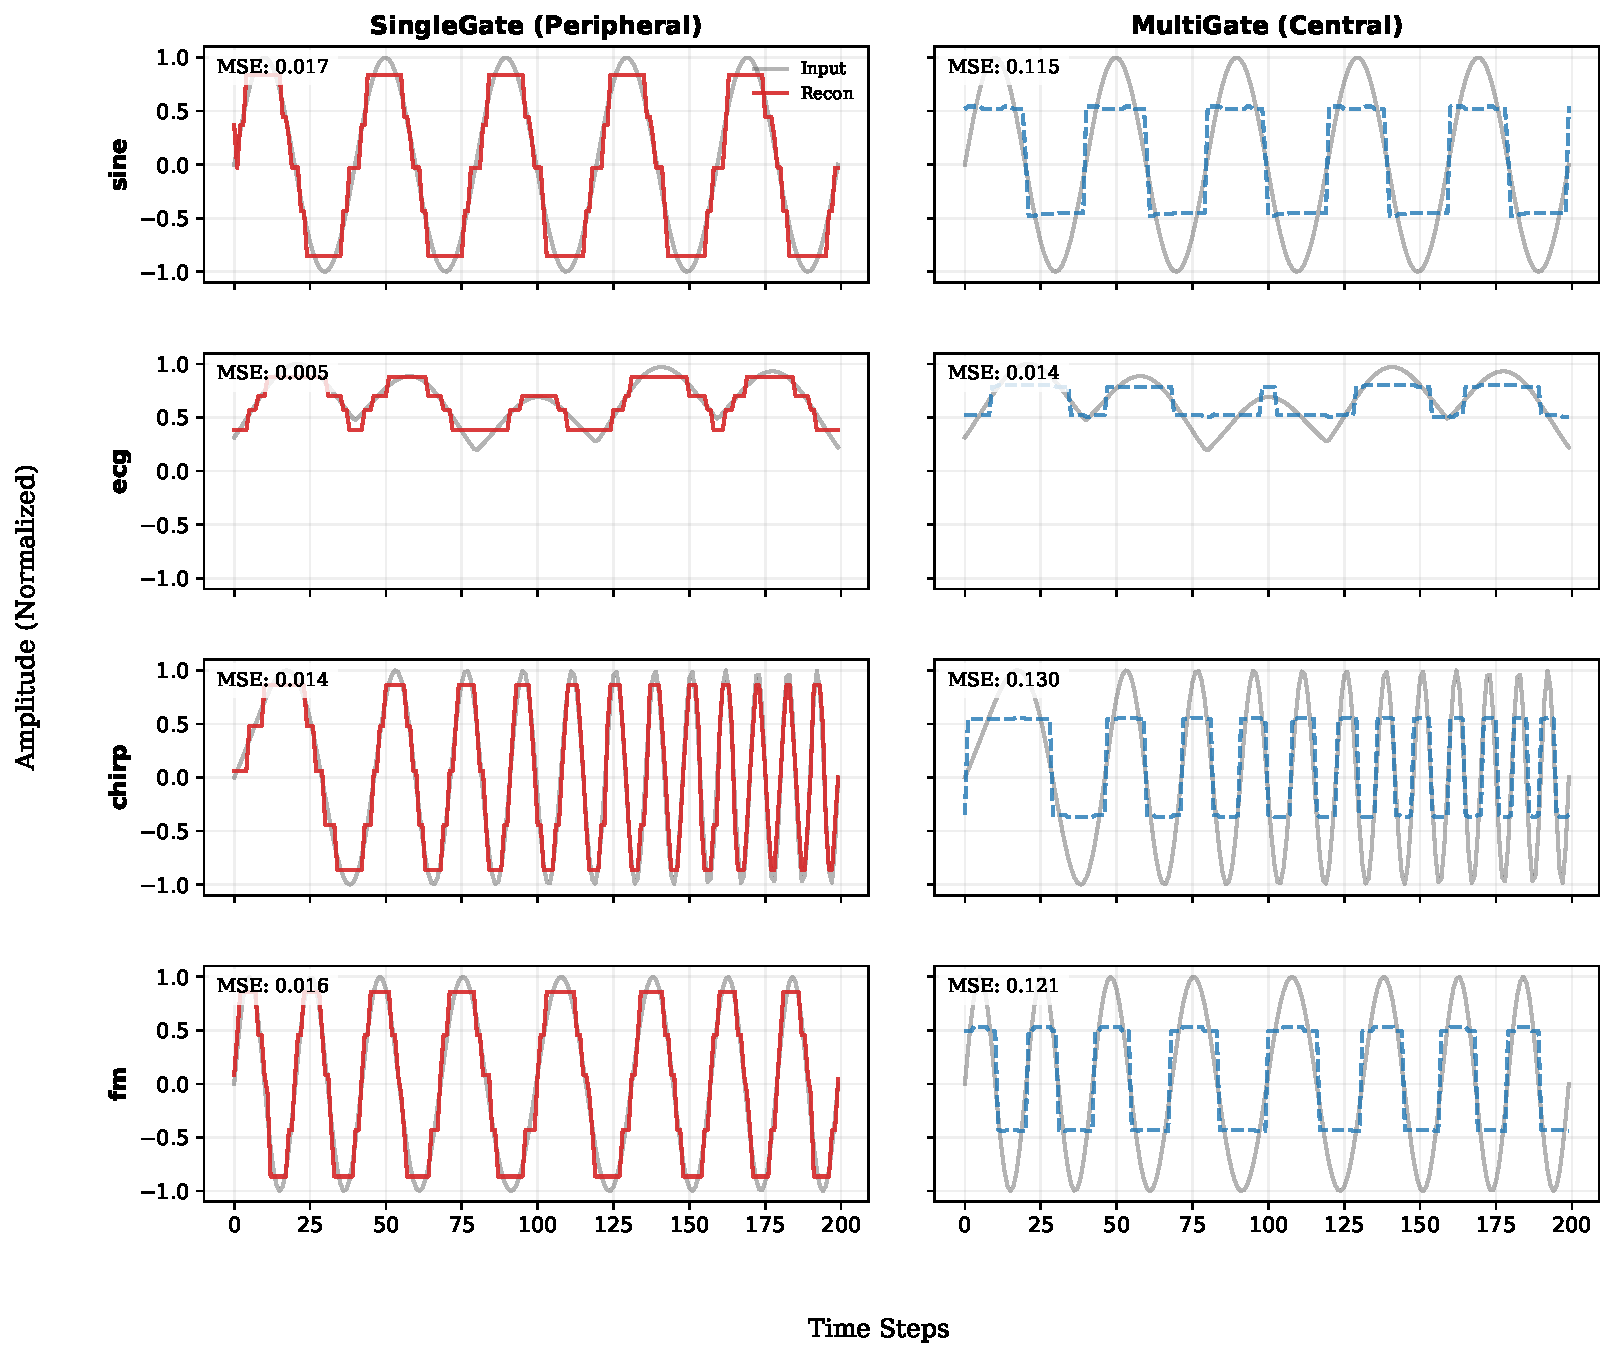
\includegraphics[width=1.0\textwidth]{results_ex1/fig_ex1_comparison.pdf}
    \caption{\textbf{Architecture Comparison (SingleGate vs. MultiGate).} 
    Representative single run (Seed=0) for four waveforms.
    The left column displays SingleGate performance, demonstrating robust phase-locking and stable discretization (red) that accurately tracks the input dynamics (gray). 
    In contrast, the right column shows MultiGate performance, which fails to capture the signal structure in a single-channel context, resulting in collapsed or noisy representations (blue dashed). 
    This visual evidence supports Hypothesis H2, confirming that complex gating mechanisms are detrimental in the absence of relational information.
    Note: MSE values shown are for this specific seed; see Table~\ref{tab:ex1} for aggregated statistics across 20 seeds.}
    \label{fig:ex1_waveforms}
\end{figure}

\begin{figure}[t]
    \centering
    \begin{minipage}{1.0\textwidth}
        \centering
        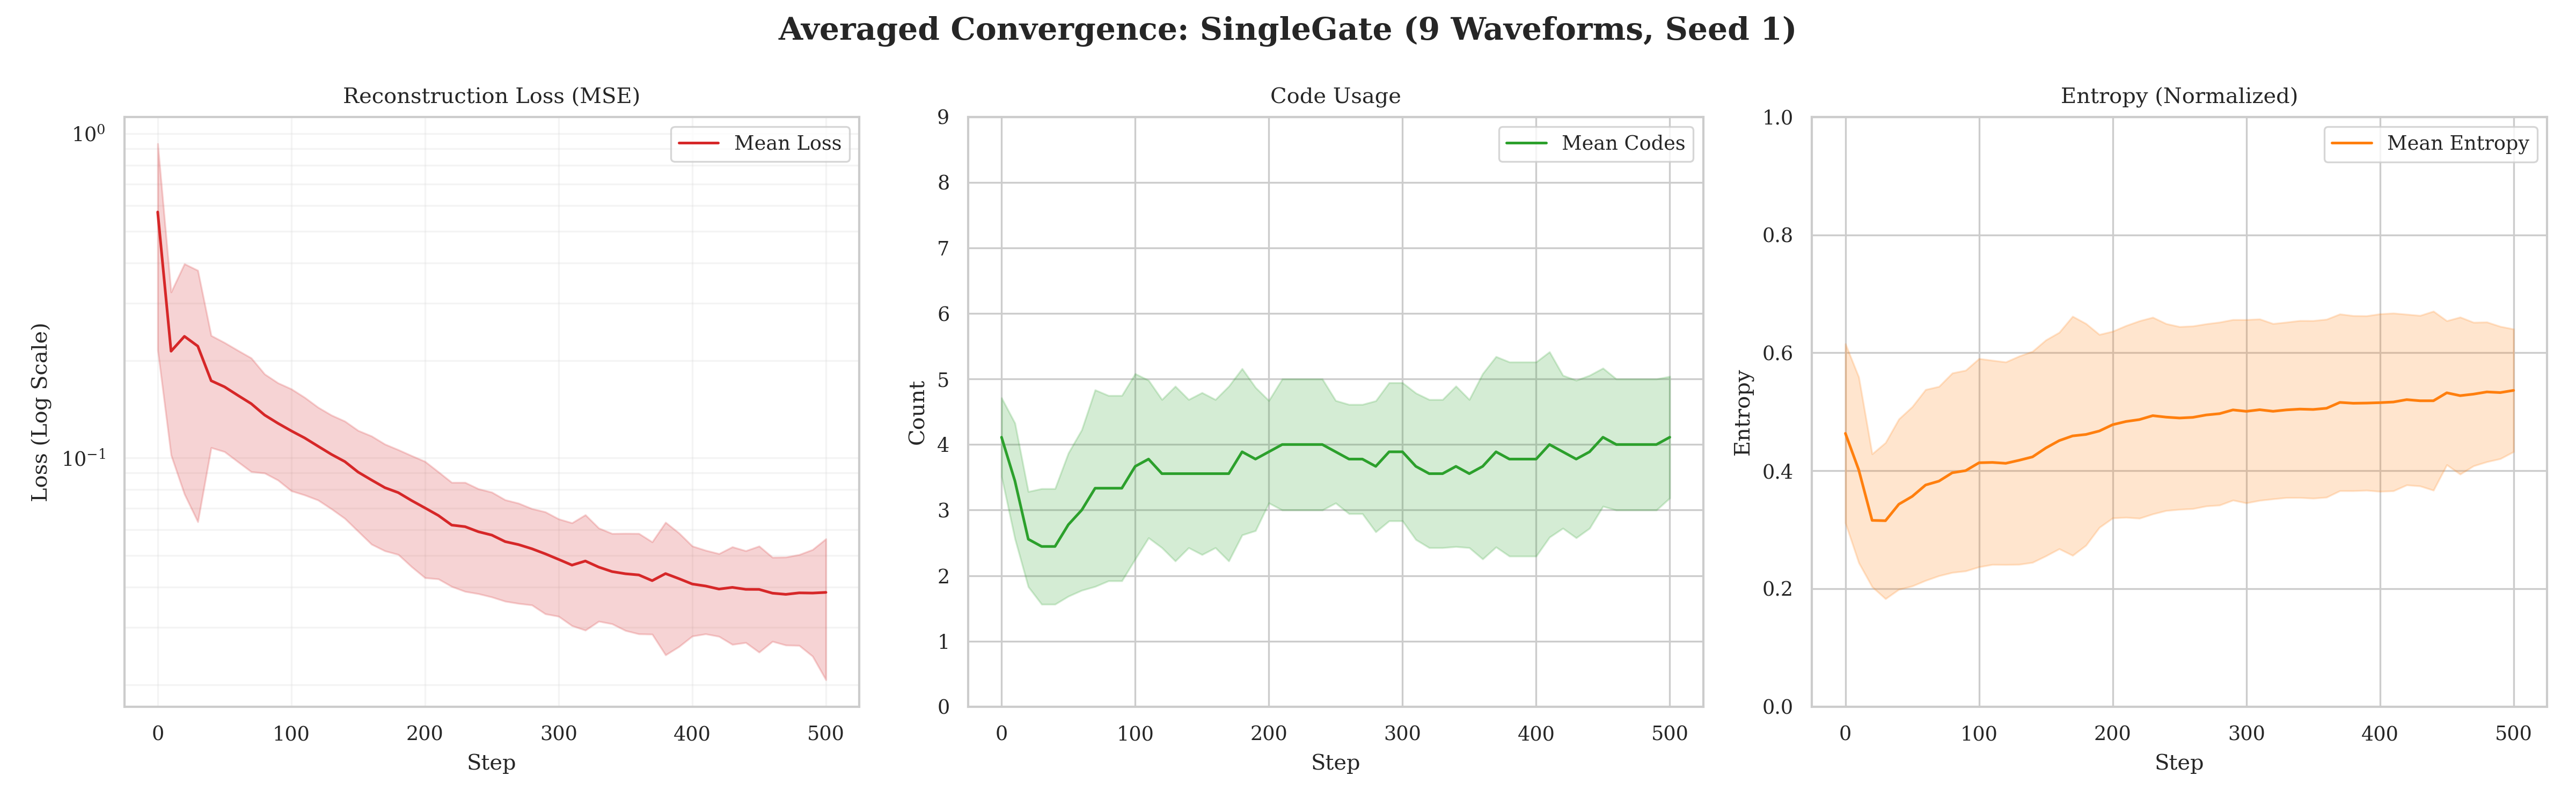
\includegraphics[width=\textwidth]{results_ex1/convergence_avg_SingleGate.png}
        \subcaption{\textbf{SingleGate (Average of 9 Waveforms).} 
        Demonstrates rapid and robust convergence. The reconstruction loss (left) drops sharply and stabilizes within 200 steps. Code usage (center) and entropy (right) show low variance (shaded area), indicating consistent behavior across diverse waveforms.}
    \end{minipage}
    
    \vspace{0.5cm}
    
    \begin{minipage}{1.0\textwidth}
        \centering
        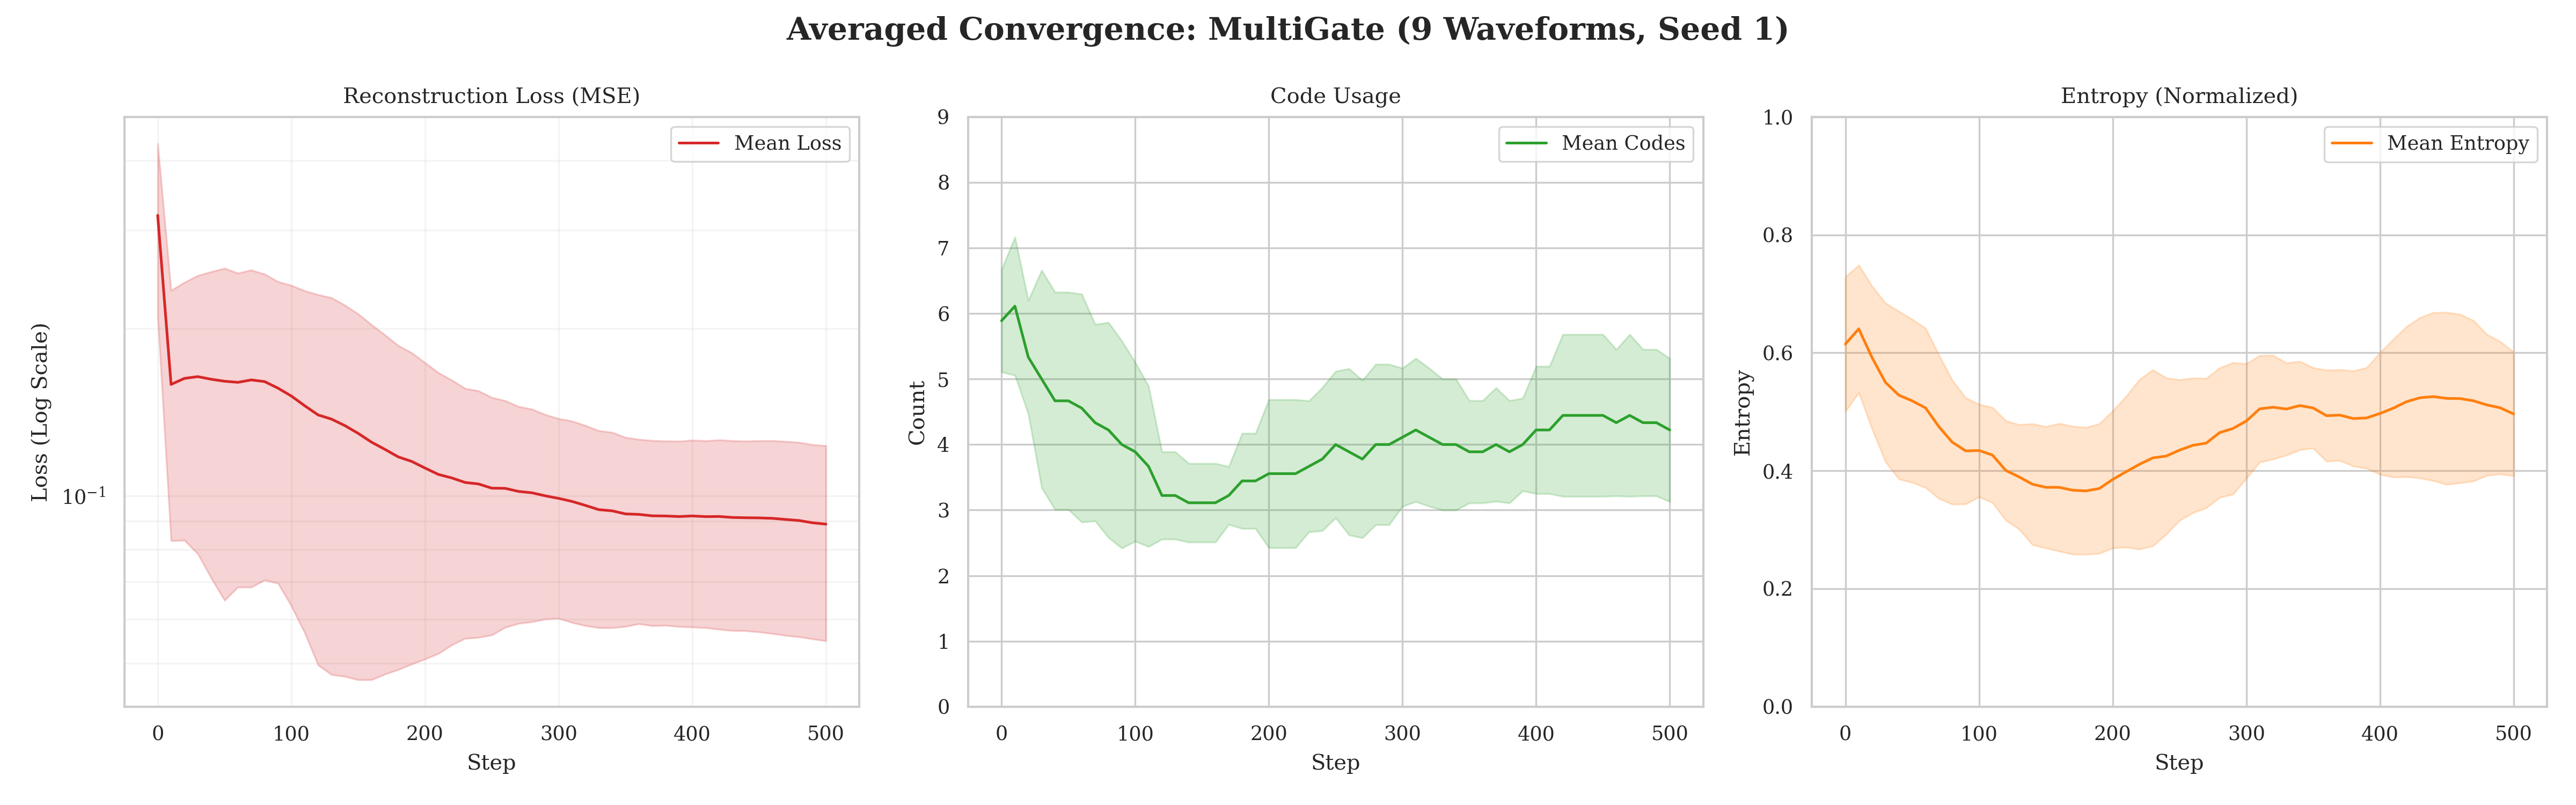
\includegraphics[width=\textwidth]{results_ex1/convergence_avg_MultiGate.png}
        \subcaption{\textbf{MultiGate (Average of 9 Waveforms).} 
        Exhibits instability and suboptimal performance. The loss remains significantly higher (note the log scale), and code usage fluctuates with high variance. This confirms that complex gating fails to lock onto simple signal dynamics without relational cues.}
    \end{minipage}
    
    \caption{\textbf{Averaged Convergence Dynamics Comparison (Steps=500).} 
    Learning trajectories averaged across all nine waveforms ($N=9$, Seed=1). Shaded regions indicate standard deviation. 
    SingleGate (a) behaves as a fast-converging dynamical integrator, while MultiGate (b) struggles to stabilize, supporting the hypothesis that minimal architecture is superior for single-channel processing.}
    \label{fig:ex1_averaged_convergence}
\end{figure}

\clearpage

%%%%%%%%%%%%%%%%%%%%%%%%%%%%%%%%%%%%%%%%%%%%%%%%%%%%%%%%%%%%%%%%%
% EXPERIMENT 2: Multi-Channel Relational Information
%%%%%%%%%%%%%%%%%%%%%%%%%%%%%%%%%%%%%%%%%%%%%%%%%%%%%%%%%%%%%%%%%
\section{Experiment 2: Multi-Channel Relational Information}

\subsection{Purpose}
Experiment 2 (EX2) validates the necessity of the MultiGate architecture for processing multi-channel signals with time-varying relationships. While Experiment 1 confirmed that SingleGate is sufficient for single-source inputs, EX2 tests the hypothesis that \textbf{independent gating (MultiGate)} is required when channels exhibit asynchronous dynamics or varying frequency ratios, which a single shared clock cannot optimally track.

\subsection{Task Design}
To evaluate the extraction of relational information, we synthesized a dual-channel dataset coupled by a time-varying frequency ratio parameter $k(t)$. Unlike Experiment 1 where features originated from a single source, here Channel 0 and Channel 1 evolve with distinct velocities. The signal dynamics are defined as follows:

\begin{itemize}
    \item \textbf{Channel 0 (Reference):} A base sinusoidal waveform acting as the physical clock reference.
    \begin{equation}
    x_{0}(t) = \sin(2\pi f_{0}t)
    \end{equation}
    \item \textbf{Channel 1 (Target):} A modulated waveform whose instantaneous frequency depends on the reference frequency scaled by $k(t)$.
    \begin{equation}
    x_{1}(t) = \sin\left(\int_{0}^{t}2\pi f_{0}k(\tau)d\tau\right)
    \end{equation}
    \item \textbf{Relational Parameter $k(t)$:} A piecewise constant function representing the hidden relationship between the channels. The sequence is divided into $N_{\text{segs}}=4$ segments, where $k$ takes a random value sampled uniformly from $[1.0, 2.0]$ for each segment. This forces the system to adapt to abrupt changes in the relational structure.
\end{itemize}

The model receives both channels as input and must learn a codebook of $K$ discrete codes that captures the relational structure. Two architectures are compared: SingleGate (shared clock for all dimensions) and MultiGate (independent clocks per channel).

\subsection{Hypothesis}
Based on the axioms of CSCT, we formulate the following hypotheses regarding architectural suitability for relational tasks:

\begin{itemize}
    \item \textbf{H1 (Failure of Shared Clock):} A SingleGate model, which enforces a single shared clock across all channels, will fail to accurately reconstruct the dual-channel signal. It will be forced to select a compromise timing that fits neither $x_0$ nor $x_1$ perfectly, resulting in discretization errors (jitter) and high reconstruction loss.
    
    \item \textbf{H2 (Success of Independent Gating):} A MultiGate model, possessing independent gate mechanisms, can assign distinct update timings to each channel. This allows Channel 0 to lock to the anchor while Channel 1 adapts its own sampling rate.
    
    \item \textbf{H3 (Relational Encoding):} The combination of discrete codes from the independent gates will implicitly encode the frequency ratio $k(t)$, allowing the system to capture the latent relational structure.
\end{itemize}

If H1--H3 are supported, combined with EX1 results, this would demonstrate a ``double dissociation'': SingleGate excels at single-channel tasks while MultiGate excels at relational tasks.

\subsection{Method}
Unlike Experiment 1 where the signal served as its own anchor, this experiment utilizes a \textbf{Reference Anchor} configuration. Channel 0 is designated as the anchor signal ($y=x_{0}$). This setup tests whether the system can utilize the physical time of the reference channel to discretize and encode the dynamics of the target channel (Channel 1).

\subsubsection{Anchor Configuration}
Reference anchor configuration: $y = x_0$. Channel 0 serves as the external temporal reference for the system.

\subsubsection{Parameters and Training}
\begin{itemize}
    \item \textbf{Model Parameters:} Codebook size $K=8$, transition penalty $\beta_{\mathrm{target}}=50$.
    \item \textbf{Training Configuration:} Sequence length $T=400$, total steps $S=1500$, $N=20$ seeds per condition. Transition penalty $\beta$ is linearly warmed up from $\beta_{\text{start}}=5$ to $\beta_{\mathrm{target}}$ during training.
    \item \textbf{Signal Parameters:} Base frequency $f_0=5.0$ Hz, $k(t) \in [1.0, 2.0]$ with $N_{\text{segs}}=4$ piecewise segments.
\end{itemize}

\subsection{Metrics}
In addition to standard reconstruction metrics, we include a task-specific metric to quantify relational understanding:

\begin{itemize}
    \item \textbf{Reconstruction Loss (MSE):}
    \begin{equation}
        \mathcal{L}_{\text{recon}} = \|x - \hat{x}\|^2
    \end{equation}
    \item \textbf{Transition Rate:} Fraction of time steps where the discrete code changes.
    \item \textbf{Unique Codes Used:} Number of distinct codes activated during processing.
    \item \textbf{Code Entropy (Normalized):} Entropy of the code distribution normalized by $\log K$.
\end{itemize}

\subsection{Results}

\begin{table}[t]
\centering
\caption{EX2 summary by $K$ and gate type (mean $\pm$ std across seeds).}
\resizebox{\columnwidth}{!}{%
\label{tab:ex2_summary}
\begin{tabular}{rlcccc}
\toprule
$K$ & Gate & Recon. loss & Transition rate & Unique codes & Code entropy (norm.) \\
\midrule
8 & MultiGate & 0.0631 $\pm$ 0.0067 & 0.102 $\pm$ 0.013 & 7.85 $\pm$ 0.36 & 0.920 $\pm$ 0.042 \\
8 & SingleGate & 0.1713 $\pm$ 0.0389 & 0.105 $\pm$ 0.016 & 6.85 $\pm$ 0.57 & 0.846 $\pm$ 0.051 \\
\addlinespace
\bottomrule
\end{tabular}
}
\end{table}


The quantitative results in Table \ref{tab:ex2_summary} summarize performance on the multi-channel relational task ($K=8$, $N=20$ seeds, 40 paired runs).
MultiGate achieves substantially lower reconstruction error than SingleGate:
$\mathrm{Recon}=0.0631$ (95\% CI [0.0601, 0.0661]) vs.\ $0.1713$ (95\% CI [0.1538, 0.1888]), with a paired difference $\Delta\mathrm{Recon}=-0.1082$ (95\% CI [-0.1267, -0.0897], $d_z=-2.561$).
By contrast, transition activity is statistically indistinguishable across architectures ($\Delta\mathrm{Trans}=-0.003$, 95\% CI [-0.011, 0.005]).
MultiGate also expresses a richer discrete repertoire, using more unique codes (7.85 vs.\ 6.85; $\Delta=1.00$, 95\% CI [0.68, 1.32]) and higher normalized code entropy (0.920 vs.\ 0.846; $\Delta=0.074$, 95\% CI [0.040, 0.109]).
These effects support the claim that multi-clock routing improves relational abstraction while maintaining comparable temporal stability.

\subsection{Discussion}

Across the $K=8$ condition with 20 seeds, MultiGate's improvement is large in magnitude ($\Delta\mathrm{Recon}=-0.1082$, $d_z=-2.561$), while transition rates remain comparable, indicating that the gain is not explained by trivial suppression of switching but by improved relational coding capacity.

The results of Experiment 2, when contrasted with Experiment 1, provide compelling evidence for the distinct functional roles of the SingleGate and MultiGate architectures proposed in CSCT.

\paragraph{Trade-off between Expressivity and Abstraction.}
Experiment 1 demonstrated that SingleGate possesses \textbf{high expressivity} for concrete physical features. By strictly synchronizing the clock with the input's velocity, it achieves robust phase-locking and high-fidelity reconstruction of single-source waveforms. However, the results of Experiment 2 reveal that this same mechanism is ill-suited for extracting \textbf{abstract relational information}.
Because SingleGate enforces a shared ``window of cognition'' across all channels, it treats the multi-channel input as a monolithic entity. It cannot separate the dynamics of the reference ($x_0$) from the target ($x_1$), and thus fails to encode the \textit{difference} or \textit{ratio} ($k(t)$) between them. This confirms that while SingleGate is ideal for the immediate, physical representation of stimuli (Peripheral System), it lacks the flexibility required for relational abstraction.

\paragraph{Architecture for Relational Discovery.}
MultiGate, conversely, excelled in Experiment 2 precisely because it decoupled the channel dynamics. By allowing independent Na$^+$/NMDA gating, the system could lock Channel 0 to the reference clock and Channel 1 to the target clock. Crucially, the \textbf{combination of discrete codes} at each time step effectively encoded the frequency ratio $k(t)$. 
This validates the core hypothesis of CSCT: the \textbf{Central System (MultiGate)} is not merely a ``more complex'' version of the Peripheral System, but a distinct architecture designed to extract latent structures (relationships) that exist \textit{between} disparate information streams.

\paragraph{Conclusion.}
The ``Double Dissociation'' observed across EX1 and EX2---where SingleGate wins on stability/efficiency for single signals, while MultiGate wins on relational extraction for coupled signals---strongly supports the biological plausibility of the proposed architectures.

\subsection{Visual Analysis}
Figure \ref{fig:ex2_vertical_stack} presents a comprehensive visual comparison of the internal representations learned by the two architectures.

% ---------------------------------------------------------
% Figure: Vertical Comparison (Aggregate Analysis & Lissajous Dynamics)
% ---------------------------------------------------------
\begin{figure}[p]
    \centering
    
    % --- 1. SingleGate: Aggregate Analysis ---
    \begin{minipage}{0.9\textwidth}
        \centering
        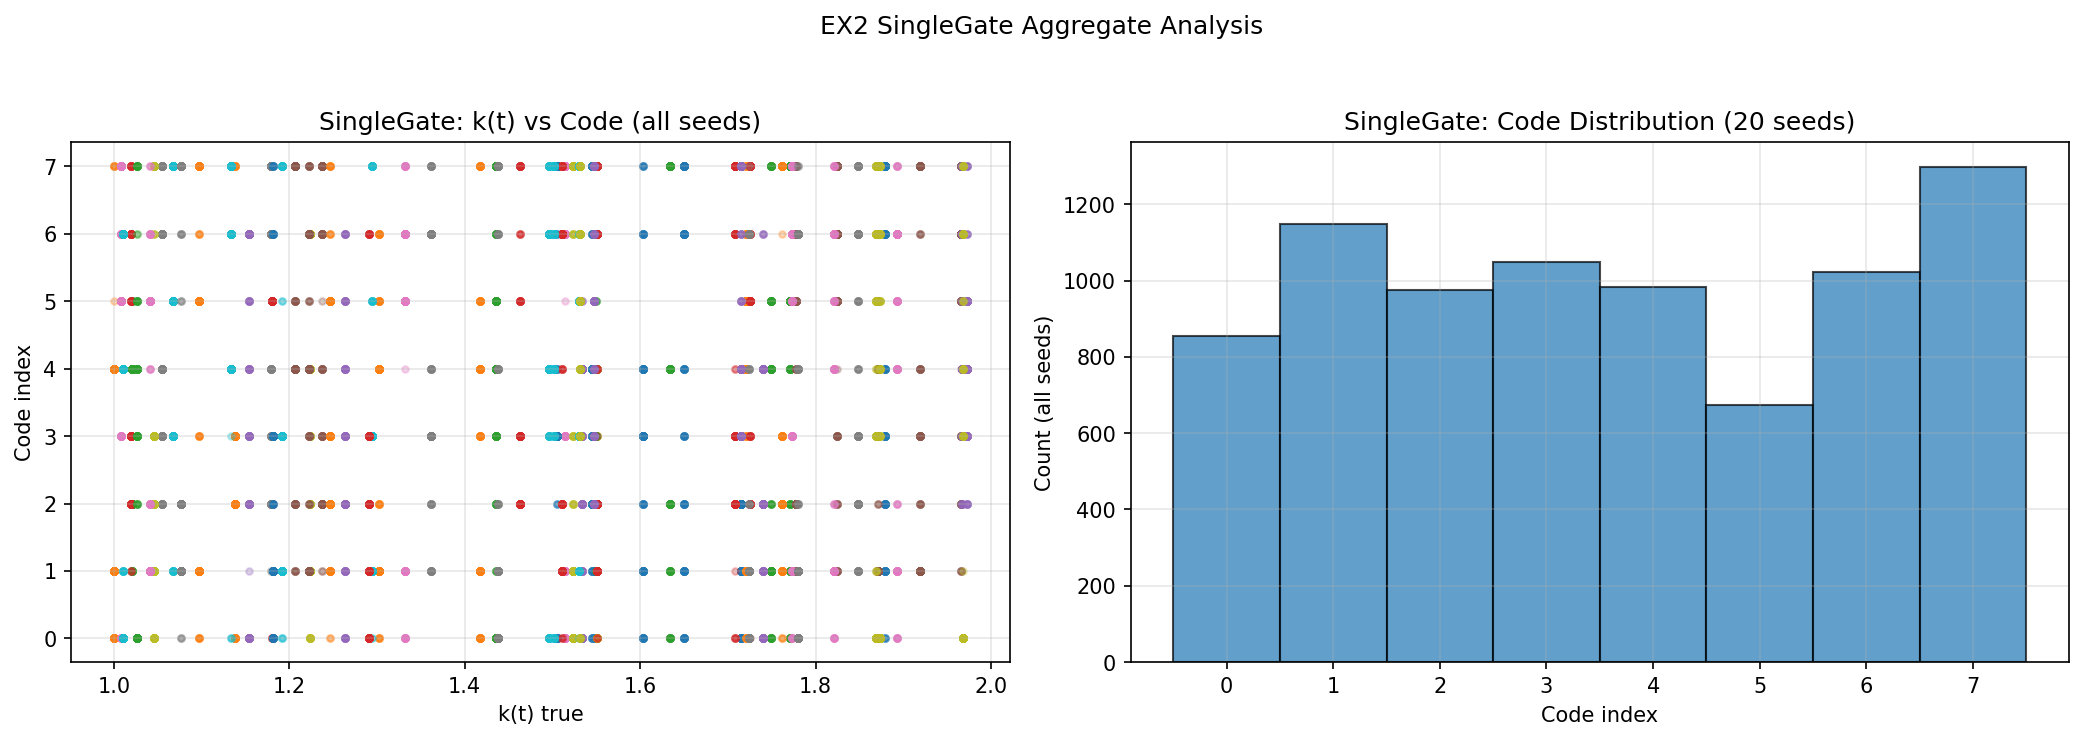
\includegraphics[width=0.85\textwidth]{results_ex2/ex2_SingleGate_aggregate.png}
        \subcaption{\textbf{SingleGate Aggregate Analysis.} 
        Weak correlation between discrete codes and $k(t)$ (left), with imbalanced histogram (right).}
        \label{fig:ex2_agg_single}
    \end{minipage}
    
    \vspace{0.1cm}
    
    % --- 2. MultiGate: Aggregate Analysis ---
    \begin{minipage}{0.9\textwidth}
        \centering
        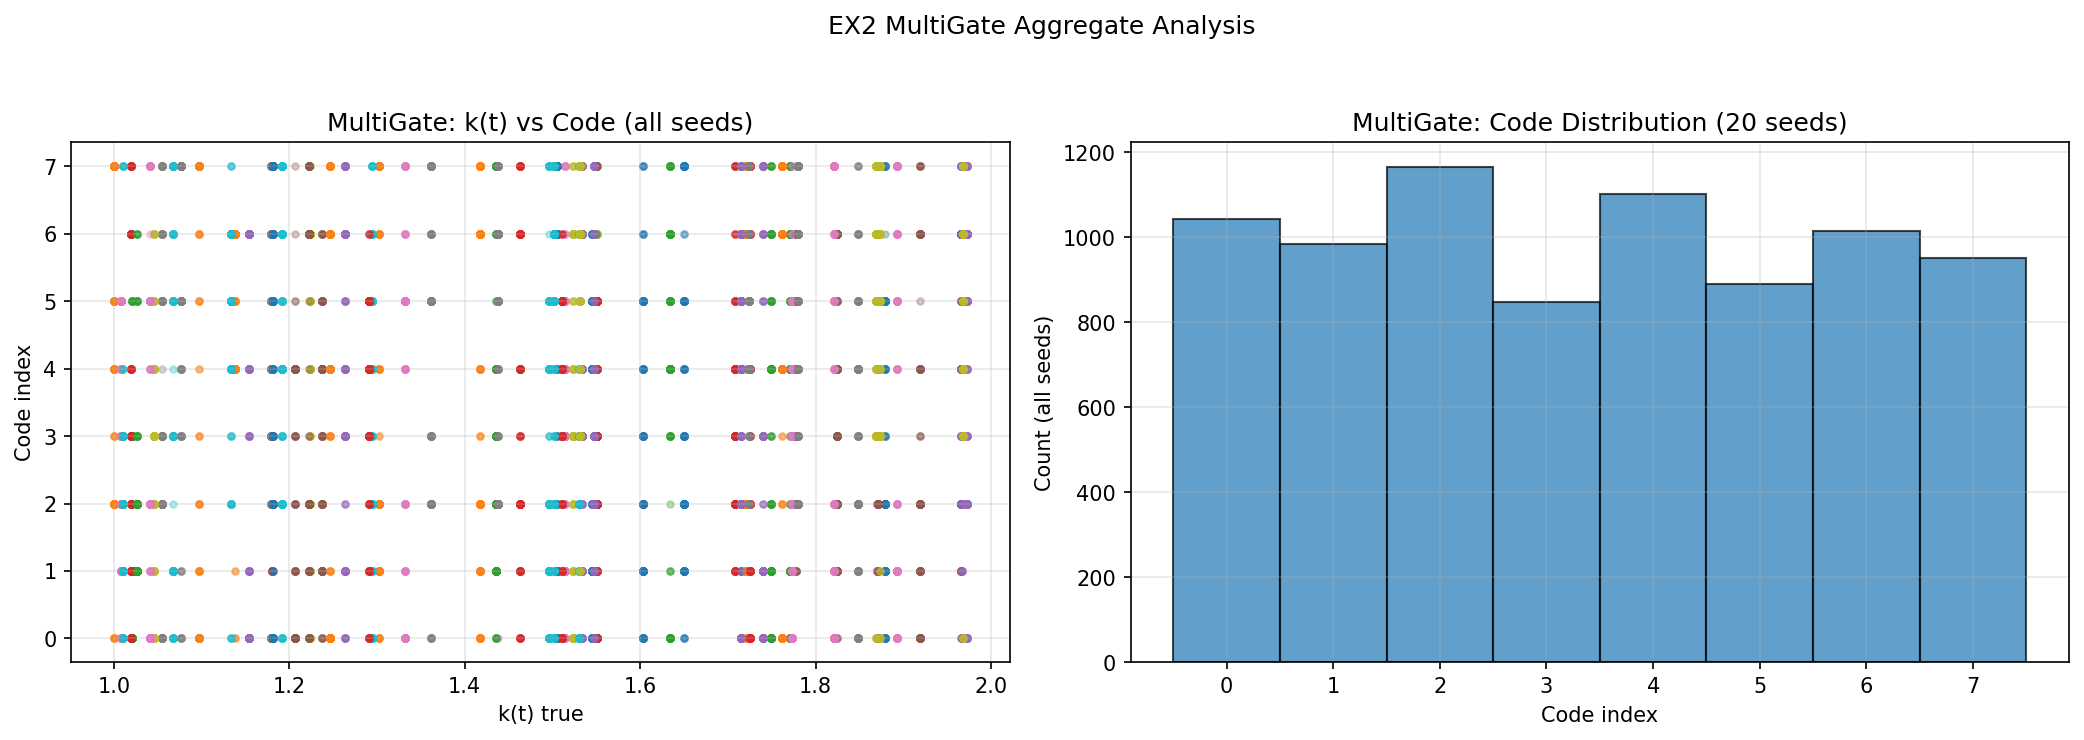
\includegraphics[width=0.85\textwidth]{results_ex2/ex2_MultiGate_aggregate.png}
        \subcaption{\textbf{MultiGate Aggregate Analysis.} 
        Structured distribution relative to $k(t)$ (left) and broader code usage (right).}
        \label{fig:ex2_agg_multi}
    \end{minipage}
    
    \vspace{0.1cm}
    
    % --- 3. SingleGate: Lissajous ---
    \begin{minipage}{0.9\textwidth}
        \centering
        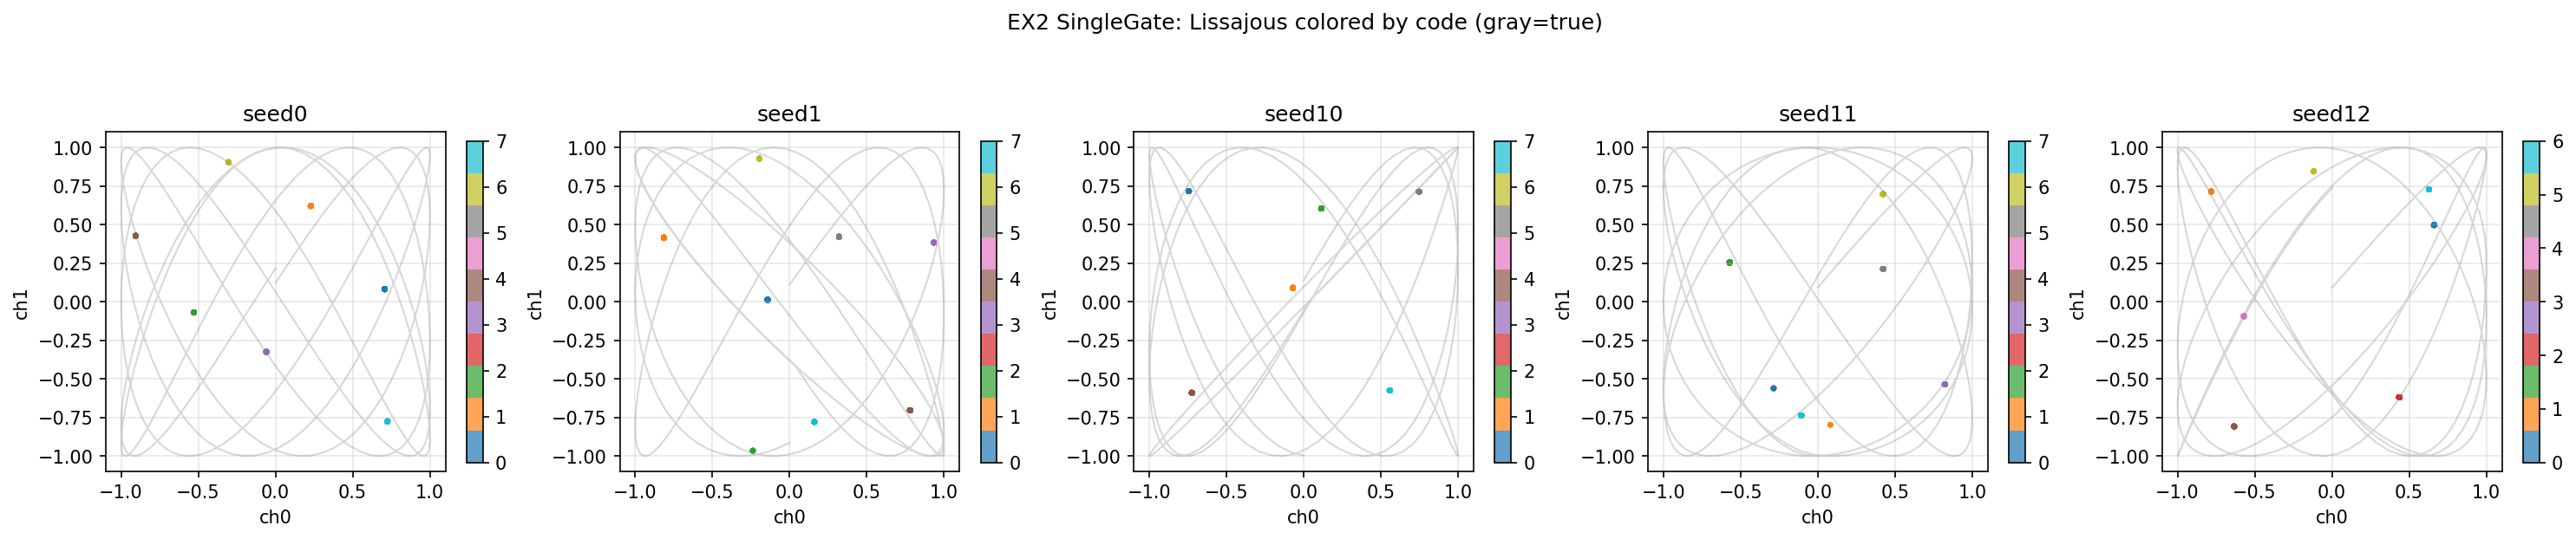
\includegraphics[width=0.85\textwidth]{results_ex2/ex2_SingleGate_lissajous.png}
        \subcaption{\textbf{SingleGate Lissajous} (representative seeds: 0, 1, 10, 11, 12). 
        Erratic clustering in phase space colored by code.}
        \label{fig:ex2_liss_single}
    \end{minipage}
    
    \vspace{0.1cm}
    
    % --- 4. MultiGate: Lissajous ---
    \begin{minipage}{0.9\textwidth}
        \centering
        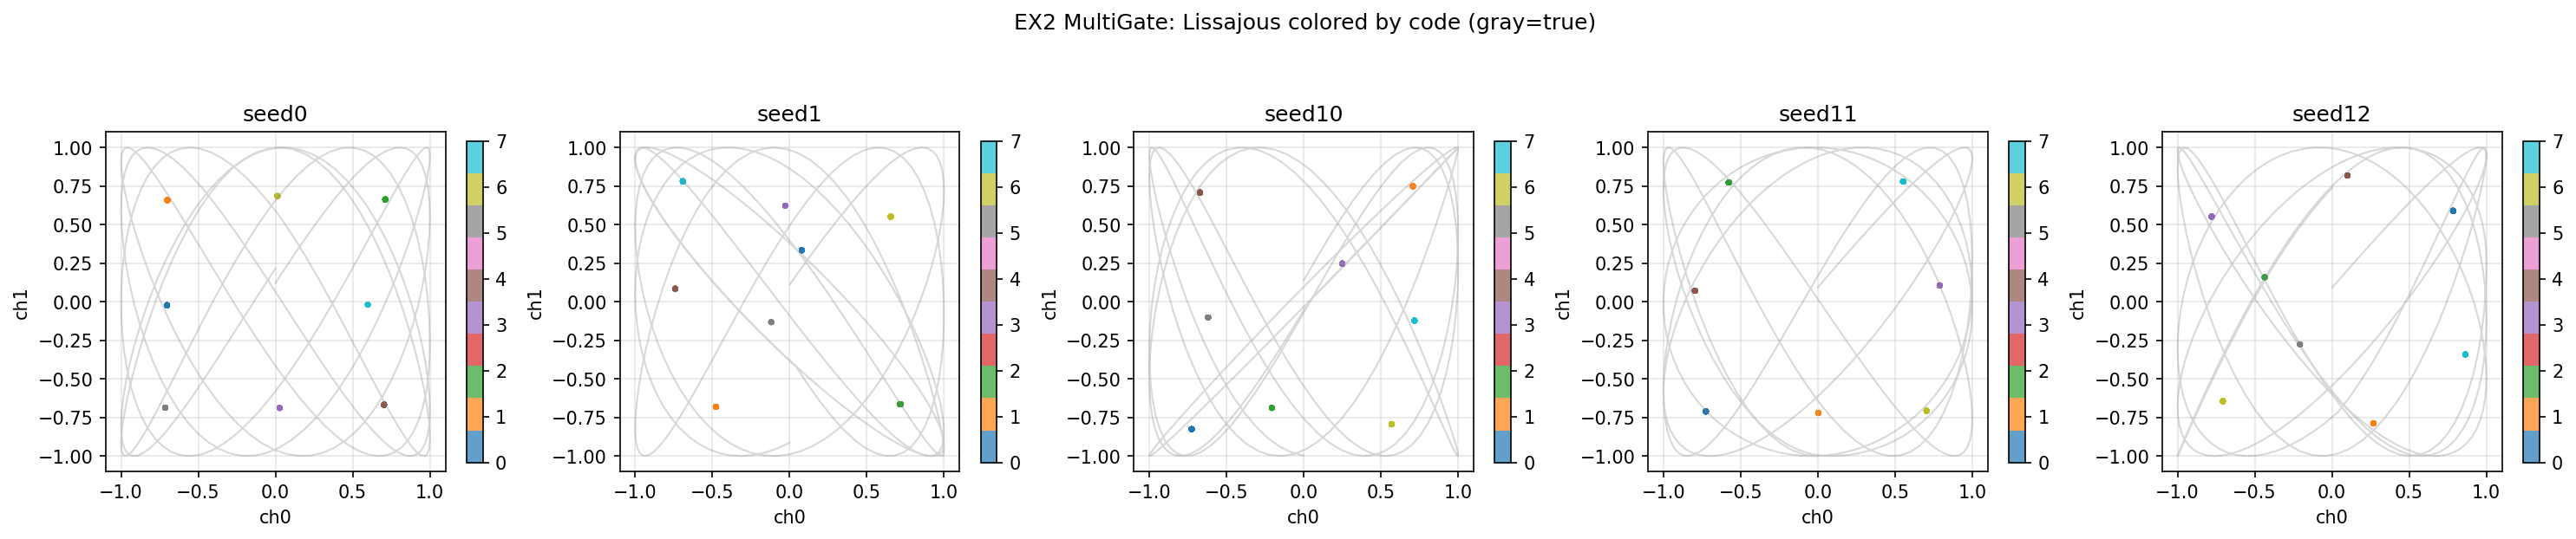
\includegraphics[width=0.85\textwidth]{results_ex2/ex2_MultiGate_lissajous.png}
        \subcaption{\textbf{MultiGate Lissajous} (representative seeds: 0, 1, 10, 11, 12). 
        Consistent code activation mapped to trajectory geometry.}
        \label{fig:ex2_liss_multi}
    \end{minipage}
    
    \caption{\textbf{Vertical Comparison of Aggregate Statistics and Phase Space Dynamics.} 
    (a, b) Aggregate analysis of $k(t)$ vs. code usage across 20 seeds. MultiGate (b) shows clearer structure than SingleGate (a).
    (c, d) Lissajous phase portraits colored by code index. MultiGate (d) demonstrates stable geometric encoding.
    Note: Aggregate plots include all 20 seeds; Lissajous plots show 5 representative seeds.}
    \label{fig:ex2_vertical_stack}
\end{figure}


\clearpage

%%%%%%%%%%%%%%%%%%%%%%%%%%%%%%%%%%%%%%%%%%%%%%%%%%%%%%%%%%%%%%%%%
% EXPERIMENT 3: K-Dependency Analysis (Discretization Geometry)
%%%%%%%%%%%%%%%%%%%%%%%%%%%%%%%%%%%%%%%%%%%%%%%%%%%%%%%%%%%%%%%%%
\section{Experiment 3: K-Dependency Analysis (Discretization Geometry)}

\subsection{Purpose}
Experiment 3 (EX3) investigates the geometric nature of the discretization performed by CSCT. Specifically, we examine how the codebook size $K$ determines the granularity of the representation. The goal is to demonstrate that the system performs a \textbf{``Lebesgue-like'' integration} (partitioning the value space/amplitude) rather than a ``Riemann-like'' integration (partitioning the time domain).

\subsection{Task Design}
To isolate the discretization geometry, we employ a minimal setup:
\begin{itemize}
    \item \textbf{Input:} A pure sine wave $x(t) = \sin(2\pi f_0 t)$ with $f_0 = 5.0$ Hz.
    \item \textbf{Architecture:} SingleGate (clean analysis without relational complexity).
    \item \textbf{Variable:} Codebook size $K \in \{2, 4, 8, 16\}$.
\end{itemize}

The model receives the sine wave as input and must learn a codebook that partitions the amplitude range into $K$ discrete regions. By varying $K$, we observe how the system refines its discretization boundaries.

\subsection{Hypothesis}
We propose that the discrete codes self-organize based on the signal's phase space topology and velocity constraints, rather than uniform temporal sampling:

\begin{itemize}
    \item \textbf{H1 ($K=2$, Sign Detection):} With minimal capacity, the fundamental partition maximizes information by capturing the sign of the signal. Transitions will align with \textbf{zero-crossings}, where the velocity (information flux) is maximal.
    
    \item \textbf{H2 (Lebesgue-like Partitioning for $K>2$):} For larger capacities, the system partitions the amplitude range into discrete bins (Lebesgue-like integration). Because transitions are suppressed near extrema by the velocity constraint (H3), the additional codes ($K \ge 4$) are preferentially allocated to partition \emph{wave slopes / amplitude gradients} rather than peak/trough switching, yielding coarse-to-fine amplitude quantization.
    
    \item \textbf{H3 (Velocity Constraint at Extrema):} Transitions are discouraged near extrema ($\dot{x}(t)\approx 0$), so transitions do not concentrate at peaks/troughs even when $K$ increases; instead, discretization refines along nonzero-slope regions.
\end{itemize}

If H1--H3 are supported, this would demonstrate that CSCT performs value-space partitioning (Lebesgue-like) rather than time-domain sampling (Riemann-like).

\subsection{Method}
We utilize a \textbf{Self-Referential Anchor} configuration ($y=x$), consistent with EX1. The input signal serves as its own clock, and the anchor gate modulation is driven by the velocity of the signal itself ($v_t = \|\dot{x}_t\|$). This ensures that no external clock dictates the timing; the discretization must emerge solely from the interaction between the signal's dynamics and the codebook constraints.

\subsubsection{Anchor Configuration}
Self-referential anchor configuration: $y = x$. The input signal serves as its own anchor.

\subsubsection{Parameters and Training}
\begin{itemize}
    \item \textbf{Model Parameters:} Architecture = SingleGate, Codebook size $K \in \{2, 4, 8, 16\}$, transition penalty $\beta_{\mathrm{target}} = 50$.
    \item \textbf{Training Configuration:} Sequence length $T=300$, total steps $S=2000$ (extended to ensure convergence of geometric boundaries), $N=20$ seeds per $K$ value. Transition penalty $\beta$ is linearly warmed up from $0$ to $\beta_{\mathrm{target}}$ during the first $S_w=200$ steps:
    \[
        \beta_{\mathrm{eff}}(s) = \beta_{\mathrm{target}} \cdot \min\!\left(1, \frac{s}{S_w}\right).
    \]
    \item \textbf{Signal Parameters:} Base frequency $f_0 = 5.0$ Hz.
\end{itemize}

\subsection{Metrics}
We analyze the distribution of transition points relative to the signal's geometry:

\begin{itemize}
    \item \textbf{Reconstruction Loss (MSE):}
    \begin{equation}
        \mathcal{L}_{\text{recon}} = \|x - \hat{x}\|^2
    \end{equation}
    \item \textbf{Transition Rate:} Fraction of time steps where the discrete code changes.
    \item \textbf{Zero-Cross Ratio:} Proportion of transitions occurring within an index tolerance window $w = \max(2, \lfloor 0.01 \cdot T \rfloor)$ around a zero-crossing event of $x(t)$.
    \item \textbf{Extrema Ratio:} Proportion of transitions occurring within the same window $w$ around an extremum (peak/trough) event, detected by sign change in $\dot{x}(t)$.
\end{itemize}

\subsection{Results}

We evaluated $K \in \{2, 4, 8, 16\}$ across $N=20$ seeds ($N=80$ total $K \times$seed runs).
Table~\ref{tab:ex3} reports the per-$K$ mean $\pm$ std across seeds.

\begin{table}[t]
\centering
\caption{Experiment 3 summary by $K$ (mean $\pm$ std across seeds).}
\label{tab:ex3}
\resizebox{\columnwidth}{!}{%
\begin{tabular}{rcccccc}
\toprule
$K$ & Recon. loss & Transition rate & Transitions & Zero-cross ratio & Extrema ratio & Other \\
\midrule
2 & $0.1005 \pm 0.0043$ & $0.034 \pm 0.003$ & $10.2 \pm 0.8$ & $1.000 \pm 0.000$ & $0.000 \pm 0.000$ & $0.0 \pm 0.0$ \\
4 & $0.0409 \pm 0.0041$ & $0.073 \pm 0.009$ & $21.8 \pm 2.6$ & $0.438 \pm 0.188$ & $0.000 \pm 0.000$ & $12.1 \pm 4.2$ \\
8 & $0.0214 \pm 0.0045$ & $0.122 \pm 0.011$ & $36.6 \pm 3.4$ & $0.449 \pm 0.048$ & $0.000 \pm 0.000$ & $20.1 \pm 2.0$ \\
16 & $0.0149 \pm 0.0015$ & $0.161 \pm 0.013$ & $48.0 \pm 4.0$ & $0.546 \pm 0.055$ & $0.000 \pm 0.000$ & $21.8 \pm 2.8$ \\
\bottomrule
\end{tabular}
}
\end{table}

Pooled across all $K \times$seed runs, the reconstruction loss was $0.0444$ (95\% CI [0.0369, 0.0519]), with transition rate $0.097$ (95\% CI [0.087, 0.108]) and $29.1$ transitions on average (95\% CI [25.9, 32.4]).
The boundary-type ratios were dominated by zero-cross events (zero-cross ratio $0.608$, 95\% CI [0.553, 0.664]), while extrema events were not detected (extrema ratio $0.000$, 95\% CI [0.000, 0.000]); the remaining events fell into the residual ``other'' category ($13.5$, 95\% CI [11.5, 15.5]).

Across $K$, reconstruction improved monotonically as codebook capacity increased:
$0.1005$ at $K=2$ (95\% CI [0.0985, 0.1024]),
$0.0409$ at $K=4$ (95\% CI [0.0390, 0.0427]),
$0.0214$ at $K=8$ (95\% CI [0.0194, 0.0234]),
and $0.0149$ at $K=16$ (95\% CI [0.0142, 0.0156]).
In parallel, the transition rate increased with $K$ (from $0.034$ at $K=2$ to $0.161$ at $K=16$), consistent with finer partitioning of the phase trajectory into more frequent discrete updates.
Notably, $K=2$ produced a degenerate regime where virtually all detected boundary events occurred at zero crossings (zero-cross ratio $1.000$), whereas for $K \ge 4$ the zero-cross ratio settled in the $0.44$--$0.55$ range, reflecting more distributed boundary formation across the signal geometry.

\subsection{Discussion}

The experimental results demonstrate that CSCT discretization is not governed by a fixed temporal clock but by the geometry of the signal's value space. Mathematically, this allows us to formulate CSCT not as a Riemann sampling process, but as a \textbf{Lebesgue-style value-partitioning} process.

\paragraph{Riemann vs. Lebesgue Discretization.}
Standard digital signal processing relies on Riemann sampling, where the time domain $\mathcal{T}$ is partitioned into fixed intervals $\Delta t$:
\begin{equation}
    x_{\text{Riemann}}(t) \approx \sum_{n} x(n\Delta t) \cdot \delta(t - n\Delta t)
\label{eq:ex3_riemann}
\end{equation}
In contrast, CSCT partitions the \textit{range} (amplitude space) $\mathcal{X}$ into $K$ disjoint regions $R_k$ defined by the codebook vectors $\mathbf{c}_k$:
\begin{equation}
    R_k = \{ x \in \mathcal{X} \mid \text{enc}(x) = k \}
\label{eq:ex3_range_partition}
\end{equation}
The system assigns a discrete code $k$ to the time intervals (sets of measure) $E_k$ where the signal falls within region $R_k$:
\begin{equation}
    E_k = \{ t \in \mathcal{T} \mid x(t) \in R_k \} = x^{-1}(R_k)
\label{eq:ex3_time_preimage}
\end{equation}
Consequently, the signal reconstruction $\hat{x}(t)$ becomes a \textbf{simple function} in the measure-theoretic sense:
\begin{equation}
    \hat{x}(t) = \sum_{k=1}^{K} \mathbf{c}_k \cdot \mathbb{I}_{E_k}(t)
\label{eq:ex3_simple_function}
\end{equation}
where $\mathbb{I}_{E_k}$ is the indicator function for the set $E_k$.

\paragraph{Capacity-Driven Refinement.}
Increasing $K$ yields more precise discretization boundaries by refining amplitude quantization primarily along nonzero-slope regions. Consistent with H3, transitions do not cluster at extrema; the extrema ratio remains near zero across $K$, while zero-crossing-related transitions dominate.

\paragraph{Conclusion.}
The reconstruction in Eq.~\eqref{eq:ex3_simple_function} is a \textbf{simple function}, the standard approximating form used in Lebesgue integration.
In particular, integrating the reconstruction yields
\[
\int_{\mathcal{T}} \hat{x}(t)\,dt = \sum_{k=1}^{K} \mathbf{c}_k \,\mu(E_k),
\]
where $\mu(E_k)$ is the Lebesgue measure (time spent) of the preimage set $E_k = x^{-1}(R_k)$.
The empirical finding that transitions concentrate near zero-crossings but not at extrema implies that large-magnitude regions are represented by stable codes whose meaning is invariant to waveform frequency, supporting \textbf{time-invariant} amplitude semantics.

\subsection{Visual Analysis}

Figure~\ref{fig:ex3_aggregate} presents aggregate statistics across all seeds, while Figure~\ref{fig:ex3_panels} shows representative discretization patterns for a single seed.

\begin{figure}[t]
    \centering
    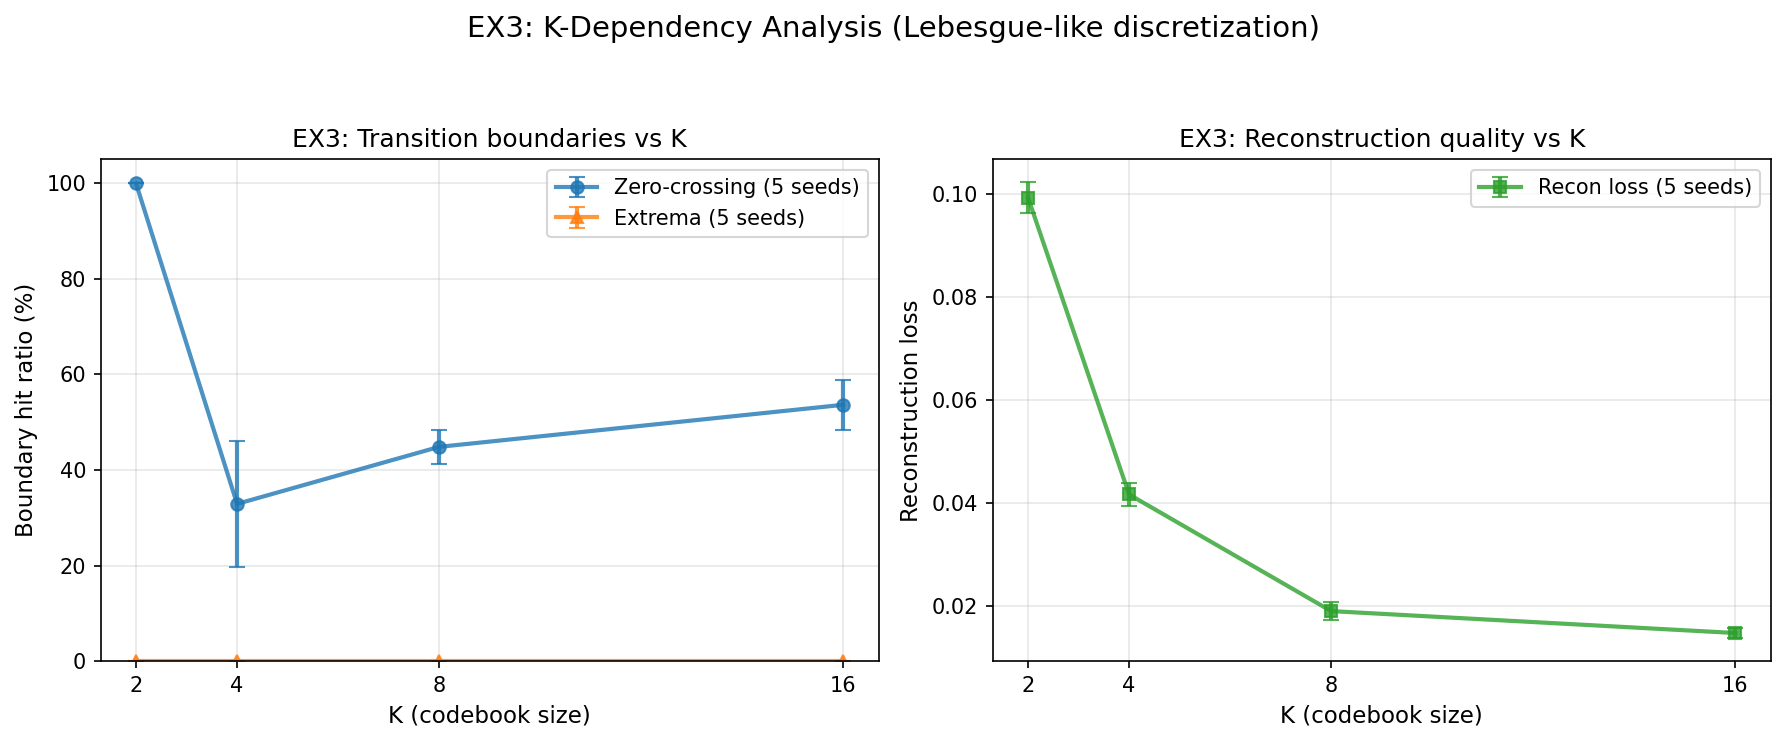
\includegraphics[width=\textwidth]{results_ex3/ex3_aggregate.png}
    \caption{\textbf{Aggregate K-Dependency (20 seeds).}
    \textbf{Left:} Transition-boundary hit ratios vs.\ $K$ (mean $\pm$ std). Zero-cross hits dominate at $K=2$ (100\%) and remain the primary transition locus across $K$, while extrema hits stay near 0\% for all $K$, indicating that transitions do not cluster at peaks/troughs.
    \textbf{Right:} Reconstruction loss decreases monotonically with $K$, demonstrating capacity-driven refinement of the discretization.}
    \label{fig:ex3_aggregate}
\end{figure}

\begin{figure}[t]
    \centering
    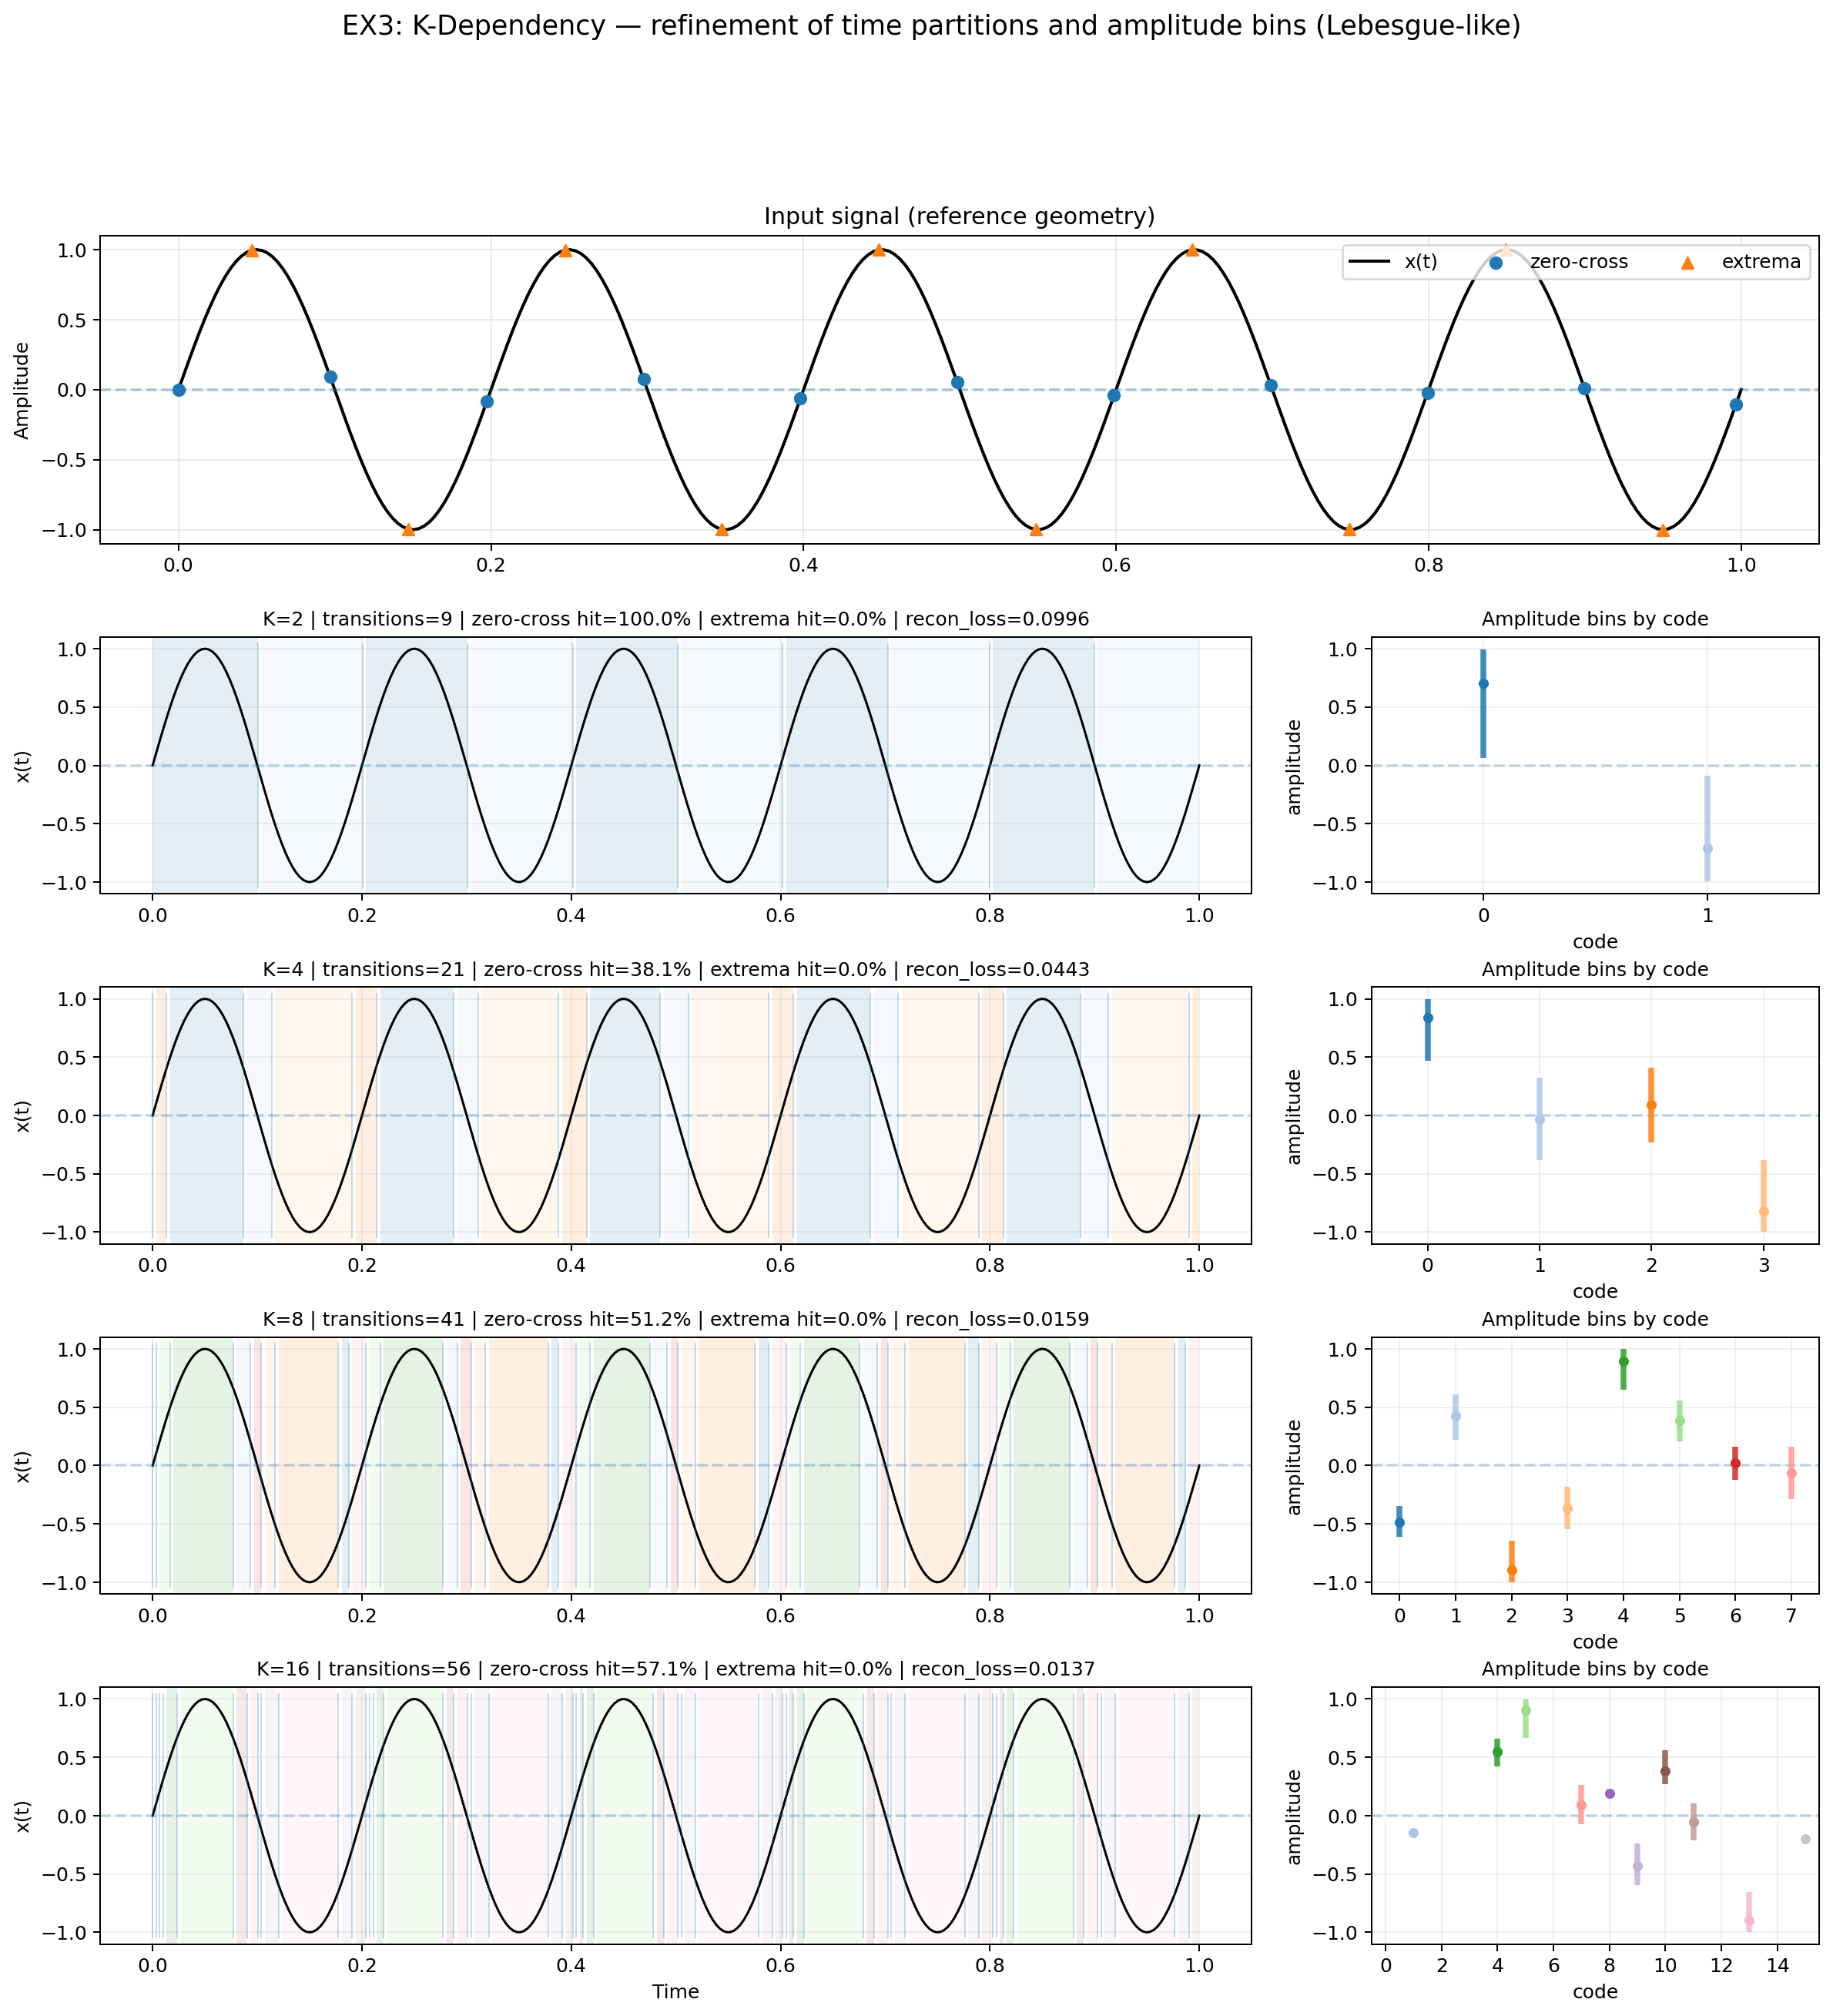
\includegraphics[width=\textwidth]{results_ex3/k_dependency_analysis.png}
    \caption{\textbf{Representative Discretization Patterns Across $K$ (Seed=0).}
    Top panel shows the input waveform with annotated zero-crossing (blue) and extrema (orange) events.
    Rows show inferred transition segments for $K \in \{2, 4, 8, 16\}$ and the corresponding amplitude bins per code.
    As $K$ increases, the number of utilized codes and amplitude bins increases, yielding finer-grained discretization and lower reconstruction error.
    Consistent with Figure~\ref{fig:ex3_aggregate}, transition boundaries concentrate near zero-crossing neighborhoods and rarely coincide with extrema, supporting Lebesgue-like refinement of amplitude bins rather than peak/trough switching.
    Note: Values shown are for this specific seed; see Table~\ref{tab:ex3} for aggregated statistics across 20 seeds.}
    \label{fig:ex3_panels}
\end{figure}

\clearpage

%%%%%%%%%%%%%%%%%%%%%%%%%%%%%%%%%%%%%%%%%%%%%%%%%%%%%%%%%%%%%%%%%
% EXPERIMENT 4: Anchor Role (Noise Floor vs. Drift)
%%%%%%%%%%%%%%%%%%%%%%%%%%%%%%%%%%%%%%%%%%%%%%%%%%%%%%%%%%%%%%%%%
\section{Experiment 4: Anchor Role (Noise Floor vs. Drift)}

\subsection{Purpose}
Experiment 4 (EX4) examines the trade-off between short-term accuracy and long-term stability in anchored vs.\ autonomous systems. The experiment tests whether external anchoring can bound error accumulation despite introducing immediate noise.

\subsection{Task Design}
The task examines a fundamental trade-off in estimation theory: the choice between an autonomous internal model (which accumulates drift over time) and an externally-anchored model (which tracks a noisy reference).

We construct a minimal scenario that isolates this trade-off:
\begin{itemize}
    \item \textbf{Target Signal:} A sine wave $x(t) = \sin(t)$ that the system must track.
    \item \textbf{Internal Model Imperfection:} The system's internal oscillator has a 3\% frequency error ($\omega_{\text{model}} = 1.03\omega_{\text{true}}$). Without external correction, this causes the internal phase to drift away from the true phase at a rate of $0.03$ rad/s.
    \item \textbf{Anchor Signal:} A noisy sawtooth wave $y(t) = \text{saw}(t) + \mathcal{N}(0, \sigma^2)$ that provides phase information corrupted by Gaussian noise. The sawtooth is chosen because its phase can be unambiguously extracted (unlike a sine wave which has phase ambiguity).
    \item \textbf{Noise Levels:} $\sigma \in \{0.05, 0.1, 0.2, 0.3\}$, spanning low to high noise regimes.
\end{itemize}

Two systems are compared:
\begin{enumerate}
    \item \textbf{Closed System:} Ignores the anchor and relies purely on internal dynamics. It avoids anchor noise but accumulates drift.
    \item \textbf{Open System:} Locks to the anchor via a phase-locked loop (PLL). It accepts anchor noise but prevents drift accumulation.
\end{enumerate}

The question is: when does anchoring become beneficial despite its noise cost?

\subsection{Hypothesis}
\begin{itemize}
    \item \textbf{H1 (Short-term Noise Cost):} The Closed System will show lower error initially due to noise filtering.
    \item \textbf{H2 (Long-term Drift Prevention):} The Open System will show lower error long-term due to drift prevention.
    \item \textbf{H3 (Crossover Point):} A crossover point $T_{\text{cross}}$ will exist where anchoring becomes beneficial, with $T_{\text{cross}}$ increasing monotonically with noise level $\sigma$.
\end{itemize}

If H1--H3 are supported, this would demonstrate that irreversible anchors provide long-term stability rather than immediate accuracy.

\subsection{Method}

\subsubsection{Anchor Configuration}
\begin{enumerate}
    \item \textbf{Closed System:} Harmonic Integrator evolving autonomously:
    \begin{equation}
        \ddot{z} = -\omega_{\text{error}}^2 z
    \end{equation}
    \item \textbf{Open System:} Phase-Locked Loop with full anchor coupling ($\alpha=1.0$):
    \begin{equation}
        \phi_t = \text{saw}^{-1}(y_t)
    \end{equation}
\end{enumerate}

\subsubsection{Parameters and Training}
\begin{itemize}
    \item \textbf{Model Type:} Mathematical Simulation (Harmonic Integrator)
    \item \textbf{Model Parameters:} Noise levels $\sigma \in \{0.05, 0.1, 0.2, 0.3\}$, frequency error $3\%$, PLL coupling $\alpha = 1.0$.
    \item \textbf{Simulation Configuration:} Sequence length $T=2000$ steps, Symplectic Euler integration, $N=20$ seeds per noise level.
    \item \textbf{Analysis Windows:} Short-term: $t < 100$; Long-term: $t > 1500$.
\end{itemize}

\subsection{Metrics}
\begin{itemize}
    \item \textbf{Short-term MSE:} Mean Squared Error for $t < 100$.
    \item \textbf{Long-term MSE:} Mean Squared Error for $t > 1500$.
    \item \textbf{Crossover Step $T_{\text{cross}}$:} Step where Open error falls below Closed error.
\end{itemize}

\subsection{Results}
We evaluated four anchor-noise levels $\sigma \in \{0.05, 0.10, 0.20, 0.30\}$ with $N=20$ seeds (total 80 condition--seed trials).
In this setup the \emph{closed} baseline is deterministic by construction (no external injection), and therefore exhibits near-zero variance across seeds in both the short-term and long-term MSE.
Table~\ref{tab:ex4} summarizes mean $\pm$ std across seeds; for prose we report pooled means with 95\% confidence intervals (normal approximation).

\begin{table}[t]
    \centering
    \caption{Experiment 4 summary by noise level (mean $\pm$ std across seeds).}
    \label{tab:ex4}

    % --- Subtable (a): Reconstruction Accuracy (MSE) ---
    \begin{subtable}{\columnwidth}
        \centering
        \caption{Reconstruction Accuracy (MSE)}
        \resizebox{\columnwidth}{!}{%
        \begin{tabular}{rcccc}
            \toprule
            $\sigma_{\mathrm{noise}}$ & Short MSE (closed) & Short MSE (open) & Long MSE (closed) & Long MSE (open) \\
            \midrule
            0.05 & $0.0174 \pm 0.0000$ & $0.0127 \pm 0.0020$ & $0.4600 \pm 0.0000$ & $0.0117 \pm 0.0009$ \\
            0.10 & $0.0174 \pm 0.0000$ & $0.0457 \pm 0.0069$ & $0.4600 \pm 0.0000$ & $0.0434 \pm 0.0032$ \\
            0.20 & $0.0174 \pm 0.0000$ & $0.1487 \pm 0.0216$ & $0.4600 \pm 0.0000$ & $0.1469 \pm 0.0095$ \\
            0.30 & $0.0174 \pm 0.0000$ & $0.2716 \pm 0.0378$ & $0.4600 \pm 0.0000$ & $0.2732 \pm 0.0168$ \\
            \bottomrule
        \end{tabular}
        }
    \end{subtable}

    \vspace{0.5cm} % Space between tables

    % --- Subtable (b): Dynamics & Stability ---
    \begin{subtable}{\columnwidth}
        \centering
        \caption{Stability and Dynamics Metrics}
        \resizebox{\columnwidth}{!}{%
        \begin{tabular}{rccccc}
            \toprule
            $\sigma_{\mathrm{noise}}$ & Short win (open) & Long win (open) & Crossover idx & Freq. error & $\alpha_{\mathrm{PLL}}$ \\
            \midrule
            0.05 & $1.00 \pm 0.00$ & $1.00 \pm 0.00$ & $87.3 \pm 7.4$ & $0.030 \pm 0.000$ & $1.000 \pm 0.000$ \\
            0.10 & $0.00 \pm 0.00$ & $1.00 \pm 0.00$ & $167.1 \pm 11.9$ & $0.030 \pm 0.000$ & $1.000 \pm 0.000$ \\
            0.20 & $0.00 \pm 0.00$ & $1.00 \pm 0.00$ & $309.2 \pm 12.0$ & $0.030 \pm 0.000$ & $1.000 \pm 0.000$ \\
            0.30 & $0.00 \pm 0.00$ & $1.00 \pm 0.00$ & $434.9 \pm 15.0$ & $0.030 \pm 0.000$ & $1.000 \pm 0.000$ \\
            \bottomrule
        \end{tabular}
        }
    \end{subtable}
\end{table}


\begin{itemize}
    \item \textbf{Short-term trade-off (H1).}
    At low noise ($\sigma=0.05$), anchoring slightly improves short-term error, with $\Delta\text{short\_mse}=\text{open}-\text{closed}=-0.0046$ (95\% CI [$-0.0055,-0.0037$]).
    For higher noise ($\sigma \ge 0.10$), the anchored estimate imports the noise floor and becomes worse in the short horizon: $\Delta\text{short\_mse}=0.0284$ (95\% CI [0.0253, 0.0315]) at $\sigma=0.10$, rising to $0.2542$ (95\% CI [0.2372, 0.2712]) at $\sigma=0.30$.
    Pooled across conditions, $\Delta\text{short\_mse}=0.1023$ (95\% CI [0.0795, 0.1251]).

    \item \textbf{Long-term grounding (H2).}
    Across all noise levels, anchoring prevents drift accumulation and yields substantially lower long-term error: pooled $\Delta\text{long\_mse}=-0.3412$ (95\% CI [$-0.3638, -0.3186$]).
    The closed integrator converges to a drift-dominated plateau (long MSE $= 0.4600$ with near-zero variance), whereas the anchored system remains bounded near the noise floor (long MSE ranging from $0.0117$ at $\sigma=0.05$ to $0.2732$ at $\sigma=0.30$).

    \item \textbf{Noise-dependent validity window (H3).}
    The crossover step increases monotonically with $\sigma$, indicating a longer ``free-run'' window before drift dominates.
    The mean crossover is $T_{\mathrm{cross}}=87.3$ (95\% CI [84.0, 90.7]) at $\sigma=0.05$ and increases to $434.9$ (95\% CI [428.2, 441.7]) at $\sigma=0.30$ (pooled mean $249.6$, 95\% CI [220.1, 279.1]).
\end{itemize}

\subsection{Discussion}

EX4 isolates the \emph{control-theoretic} role of an external anchor: it bounds error over long horizons by preventing unobserved drift in an internal integrator.
When the external mapping is sufficiently direct (low noise), anchoring can be beneficial even in the short term; as the noise floor rises, anchoring becomes a long-term necessity rather than a short-term advantage.

\paragraph{Implications for Axiom A4.}
These findings justify the ``Irreversible Anchor'' axiom from a control-theoretic perspective. The anchor is ``irreversible'' not because it is perfect, but because it provides the only reference frame capable of bounding the error of an imperfect internal model over infinite time.

\paragraph{Biological Analogy.}
This trade-off mirrors sensory calibration in biological systems: internal models (e.g., vestibular integration) are accurate short-term but drift without external correction (e.g., visual landmarks). The anchor functions as a noisy but grounded reference that prevents unbounded error accumulation.

\subsection{Visual Analysis}

Figure~\ref{fig:ex4_main} presents aggregate statistics across all seeds, while Figure~\ref{fig:ex4_mechanism} shows the mechanistic details for representative runs.

\begin{figure}[t]
    \centering
    \begin{minipage}{1.0\textwidth}
        \centering
        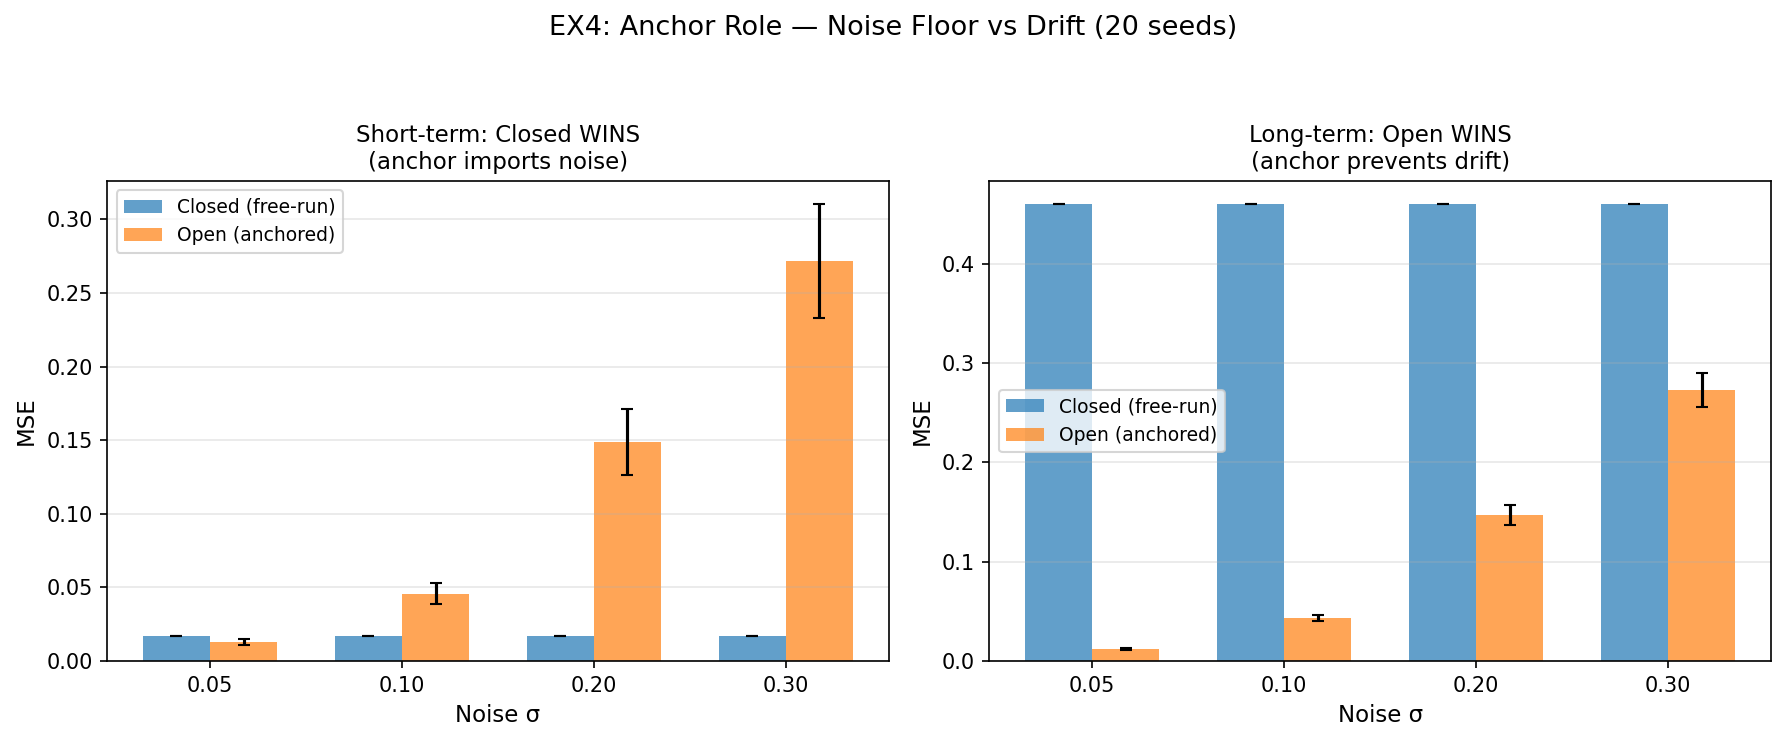
\includegraphics[width=\textwidth]{results_ex4/ex4_aggregate.png}
        \subcaption{\textbf{Aggregate Trade-off (20 seeds).}
        \textbf{Left (Short-term):} Closed wins for $\sigma \ge 0.10$ because Open imports anchor noise.
        \textbf{Right (Long-term):} Open wins across all $\sigma$ by preventing drift accumulation.}
        \label{fig:ex4_aggregate}
    \end{minipage}
    
    \vspace{0.4cm}
    
    \begin{minipage}{1.0\textwidth}
        \centering
        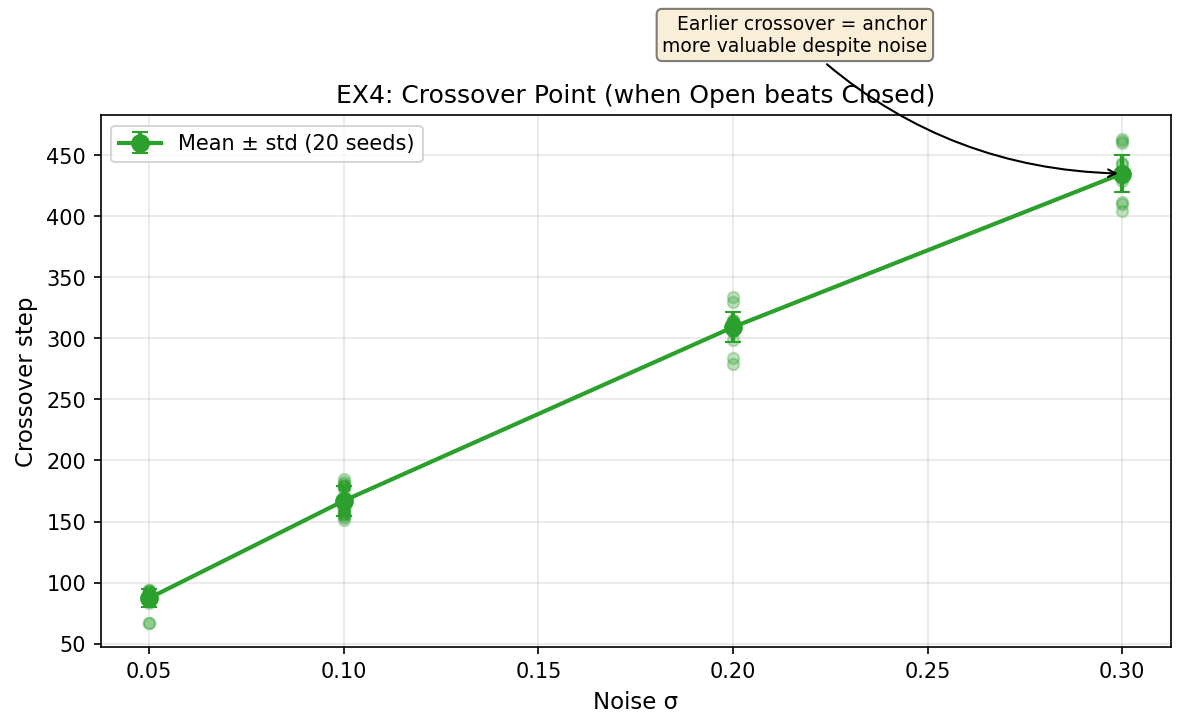
\includegraphics[width=\textwidth]{results_ex4/ex4_crossover.png}
        \subcaption{\textbf{Crossover Point $T_{\mathrm{cross}}$ vs.\ Noise (20 seeds).}
        As $\sigma$ increases, $T_{\mathrm{cross}}$ shifts later, quantifying a noise-dependent validity window for internal free-run dynamics.}
        \label{fig:ex4_crossover}
    \end{minipage}
    
    \caption{\textbf{EX4: Anchor Role---Noise Floor vs.\ Drift.}
    Panel (a) shows the core trade-off: anchors degrade immediate accuracy via noise import but dominate long-term by suppressing drift.
    Panel (b) summarizes this trade-off as crossover step $T_{\mathrm{cross}}$.}
    \label{fig:ex4_main}
\end{figure}

\begin{figure}[t]
    \centering
    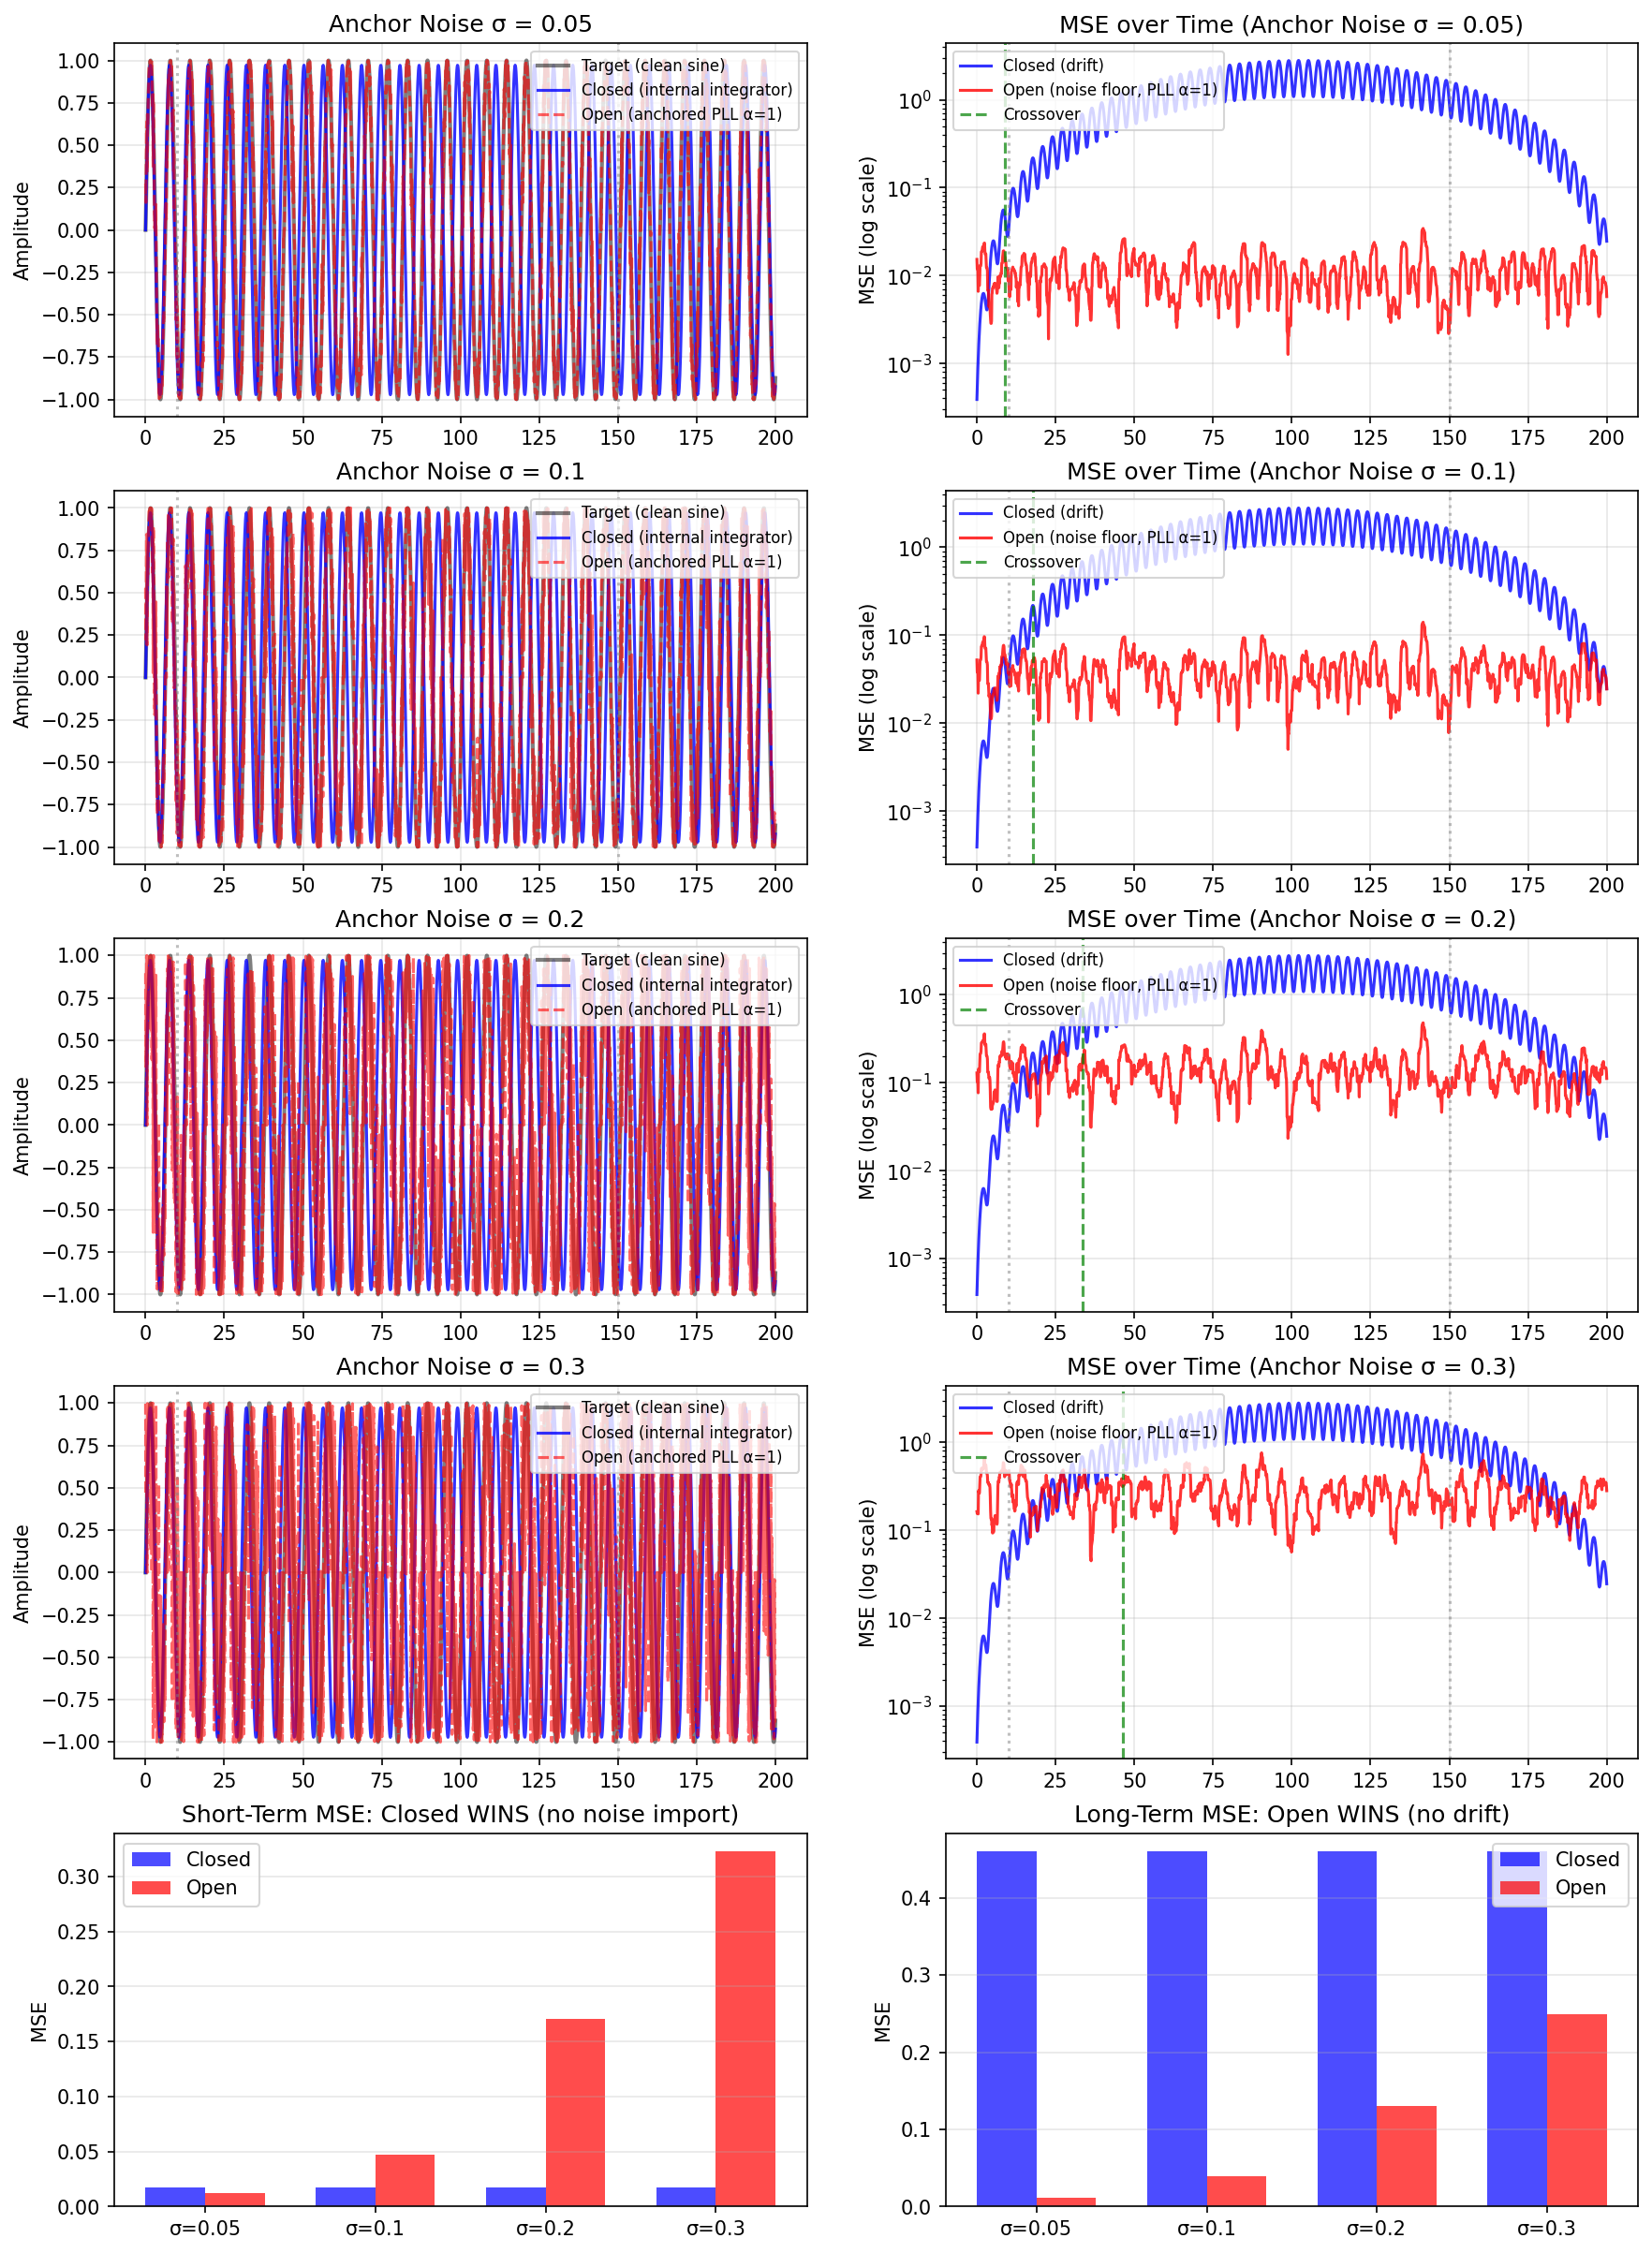
\includegraphics[width=\textwidth]{results_ex4/ex4_noise_floor.png}
    \caption{\textbf{Mechanistic View (Seed=0).}
    For each $\sigma$, left panels show waveforms (target vs.\ closed vs.\ open); right panels show per-step MSE with crossover.
    Closed error grows due to drift; open error is bounded by the noise floor.}
    \label{fig:ex4_mechanism}
\end{figure}


\clearpage

%%%%%%%%%%%%%%%%%%%%%%%%%%%%%%%%%%%%%%%%%%%%%%%%%%%%%%%%%%%%%%%%%
% EXPERIMENT 5: Binding Problem (Module Synchronization)
%%%%%%%%%%%%%%%%%%%%%%%%%%%%%%%%%%%%%%%%%%%%%%%%%%%%%%%%%%%%%%%%%
\section{Experiment 5: Binding Problem (Module Synchronization)}

\subsection{Purpose}
Experiment 5 (EX5) examines whether a shared anchor clock can preserve relative phase relationships between modules despite independent frequency drifts. This addresses the classic ``binding problem'' in cognitive science: how distributed processing modules maintain coherent representations without direct communication.

\subsection{Task Design}
The ``binding problem'' is a classic challenge in cognitive science: how does the brain integrate information from separate processing modules into a unified percept? For example, when perceiving a red apple, how are the color (processed in one area) and shape (processed in another) bound together as belonging to the same object?

EX5 tests a specific hypothesis: that binding can be achieved through \textit{shared temporal reference} rather than direct inter-module communication. If two modules independently lock to the same external clock, their internal states will remain synchronized even without exchanging information directly.

The task setup is:
\begin{itemize}
    \item \textbf{Target Signals:} Two sine waves with a fixed phase offset:
    \begin{equation}
        x_0(t) = \sin(t), \quad x_1(t) = \sin(t + \phi)
    \end{equation}
    \item \textbf{Binding Relation:} The phase difference $\phi = 1.5$ rad represents the ``relational structure'' that must be preserved. If this phase relationship drifts, the binding is lost.
    \item \textbf{Drift Condition:} Each module's internal oscillator has a frequency error of $\pm 1.5\%$ in \emph{opposite directions}. Without correction, the phase difference will drift over time, destroying the binding.
\end{itemize}

Two conditions are compared:
\begin{enumerate}
    \item \textbf{Closed Model:} Two independent oscillators with no shared reference. Each drifts according to its own frequency error.
    \item \textbf{Open Model:} Both oscillators lock to a common (noisy) anchor clock via phase-locked loops (PLLs). They never communicate directly, but both track the same external reference.
\end{enumerate}

\subsection{Hypothesis}
\begin{itemize}
    \item \textbf{H1 (Unbounded Drift without Anchor):} Without shared anchor, relative phase error will grow unbounded as modules drift apart.
    \item \textbf{H2 (Bounded Error with Anchor):} With shared anchor, relative phase error will remain bounded despite individual noise, preserving the binding relation.
\end{itemize}

If H1--H2 are supported, this would demonstrate that binding can emerge from shared temporal reference without direct inter-module communication.

\subsection{Method}

\subsubsection{Anchor Configuration}
\begin{enumerate}
    \item \textbf{Closed Model:} Two independent Harmonic Integrators with opposite frequency errors.
    \item \textbf{Open Model:} Both integrators lock to a common anchor phase:
    \begin{equation}
        \phi_{\text{anchor}}(t) = t + \eta(t), \quad \eta(t) \sim \mathcal{N}(0, \sigma_{\text{anchor}}^2)
    \end{equation}
    with PLL correction:
    \begin{equation}
        \Delta\phi_i(t) = \alpha \cdot \text{wrap}_{\pi}\left(\phi_{\text{anchor}}(t) - \phi_{\text{model},i}(t)\right)
    \end{equation}
\end{enumerate}

\subsubsection{Parameters and Training}
\begin{itemize}
    \item \textbf{Model Type:} Mathematical Simulation (Dual Harmonic Integrators)
    \item \textbf{Model Parameters:} PLL coupling $\alpha = 0.1$, target phase difference $\phi = 1.5$ rad.
    \item \textbf{Simulation Configuration:} Sequence length $T=2000$ steps, frequency errors $\epsilon_0 = +1.5\%$, $\epsilon_1 = -1.5\%$ (opposite directions), anchor noise $\sigma_{\text{anchor}} = 0.1$ rad, $N=20$ seeds.
    \item \textbf{Analysis Windows:} Short-term: $t < 200$; Long-term: $t > 1600$.
\end{itemize}

\subsection{Metrics}
\begin{itemize}
    \item \textbf{Binding Error:}
    \begin{equation}
        E_{\text{bind}}(t) = \left| \text{wrap}_{\pi}\left( \left(\hat{\phi}_1(t) - \hat{\phi}_0(t)\right) - \phi_{\text{true}} \right) \right|
    \end{equation}
    \item \textbf{Phase-Locking Value (PLV):}
    \begin{equation}
        \text{PLV}_{\text{late}} = \left| \frac{1}{|\mathcal{T}_{\text{late}}|} \sum_{t \in \mathcal{T}_{\text{late}}} \exp\left( j \cdot \text{wrap}_{\pi}\left((\hat{\phi}_1(t) - \hat{\phi}_0(t)) - \phi_{\text{true}}\right) \right) \right|
    \end{equation}
    \item \textbf{Stability Duration $T_{\text{stable}}$:} Fraction of steps where $E_{\text{bind}}(t) < 0.3$ rad.
    \item \textbf{Reconstruction MSE:} Mean squared error between predicted and target waveforms.
\end{itemize}

\subsection{Results}
We evaluated the Open (anchored) and Closed (autonomous) synchronization modes with $N=20$ seeds (paired by seed).
The quantitative results are summarized in Table~\ref{tab:ex5_results}.
In this configuration, the Closed baseline is \emph{deterministic} (fixed initial mismatch and no corrective anchor), hence its across-seed variance is effectively zero; we therefore emphasize paired differences $\Delta$ with confidence intervals.

\begin{table}[t]
    \centering
    \caption{\textbf{Experiment 5 Results (mean $\pm$ std).} $n_{\mathrm{seeds}}=20$.}
    \label{tab:ex5_results}

    % --- Subtable (a): MSE Metrics ---
    \begin{subtable}{\columnwidth}
        \centering
        \caption{Reconstruction Error (MSE)}
        \resizebox{\columnwidth}{!}{%
        \begin{tabular}{lccc}
            \toprule
            \textbf{Condition} & $\mathrm{MSE}^{\mathrm{early}}$ & $\mathrm{MSE}^{\mathrm{late}}$ & $\mathrm{MSE}^{\mathrm{total}}$ \\
            \midrule
            Closed & $0.0236$ & $3.6974$ & $1.8593$ \\
            Open   & \textbf{0.0082 $\pm$ 0.0014} & \textbf{0.0090 $\pm$ 0.0011} & \textbf{0.0089 $\pm$ 0.0005} \\
            \bottomrule
        \end{tabular}
        }
    \end{subtable}

    \vspace{0.4cm} % Space between tables

    % --- Subtable (b): Synchronization Dynamics ---
    \begin{subtable}{\columnwidth}
        \centering
        \caption{Synchronization \& Phase Dynamics}
        \resizebox{\columnwidth}{!}{%
        \begin{tabular}{lccc}
            \toprule
            \textbf{Condition} & $T_{\mathrm{stable}}$ (Duration) & $\mathrm{PLV}_{\mathrm{late}}$ (Phase Lock) & $\varepsilon_{\phi}^{\mathrm{late}}$ (Phase Error) \\
            \midrule
            Closed & $0.1$ & $0.935$ & $0.934$ \\
            Open   & \textbf{1.0} & \textbf{0.998} & \textbf{0.043 $\pm$ 0.002} \\
            \bottomrule
        \end{tabular}
        }
    \end{subtable}
\end{table}


Across seeds, Open achieves stable phase binding with low reconstruction error:
$\mathrm{MSE}^{\mathrm{early}}=0.0082$ (95\% CI [0.0076, 0.0088]),
$\mathrm{MSE}^{\mathrm{late}}=0.0090$ (95\% CI [0.0085, 0.0095]),
and $\mathrm{MSE}^{\mathrm{total}}=0.0089$ (95\% CI [0.0087, 0.0091]).
It maintains near-perfect late synchrony ($\mathrm{PLV}_{\mathrm{late}}=0.998$; 95\% CI [0.998, 0.998]) and a small late phase error ($\varepsilon_{\phi}^{\mathrm{late}}=0.043$; 95\% CI [0.042, 0.043]), with stability duration saturating at $T_{\mathrm{stable}} \approx 1.0$.

By contrast, Closed rapidly decoheres: while $\mathrm{MSE}^{\mathrm{early}}=0.0236$,
the long-horizon tracking collapses ($\mathrm{MSE}^{\mathrm{late}}=3.6974$, $\mathrm{MSE}^{\mathrm{total}}=1.8593$) with large late phase error ($\varepsilon_{\phi}^{\mathrm{late}}=0.934$) and reduced synchrony ($\mathrm{PLV}_{\mathrm{late}}=0.935$).
The paired differences (Open$-$Closed) confirm a decisive long-term advantage:
$\Delta \mathrm{MSE}^{\mathrm{late}}=-3.6884$ (95\% CI [$-3.6889, -3.6879$]),
$\Delta T_{\mathrm{stable}}=+0.9$ (95\% CI [0.9, 0.9]),
and $\Delta \varepsilon_{\phi}^{\mathrm{late}}=-0.891$ (95\% CI [$-0.892, -0.890$]).

\subsection{Discussion}

Experiment 5 provides a mechanism-level solution to the ``Binding Problem'' in distributed cognitive architectures.

\paragraph{Implicit Synchronization without Direct Communication.}
The fundamental challenge of binding is maintaining coherent relationships between spatially distributed modules that process different attributes. Our results demonstrate that \textbf{direct communication between modules is unnecessary} for binding. Instead, by locking to a common environmental anchor (Axiom A4), disjoint modules achieve \textit{implicit synchronization}. The shared anchor acts as a ``temporal glue,'' ensuring that the internal clocks of all modules tick at the same effective rate, thereby preserving their relative phase offsets (the bound information).

\paragraph{Noise vs.\ Drift Trade-off in Binding.}
Comparing EX4 and EX5 offers a deeper insight. In EX4, we saw that an anchor introduces short-term noise. However, in EX5, we see that this noise is a necessary price for inter-module coherence. A closed system might be smoother locally, but it inevitably disintegrates globally due to drift. The Open system accepts the jitter of the anchor to gain the global stability required for unified perception. This suggests that biological systems prioritize \textbf{temporal coordination} over absolute precision, utilizing environmental rhythms to bind disparate neural activities into a coherent whole.

\subsection{Visual Analysis}

Figure~\ref{fig:ex5_aggregate} presents aggregate statistics across all seeds, while Figure~\ref{fig:ex5_binding_dynamics} shows the mechanistic details for a representative run.

\begin{figure}[t]
    \centering
    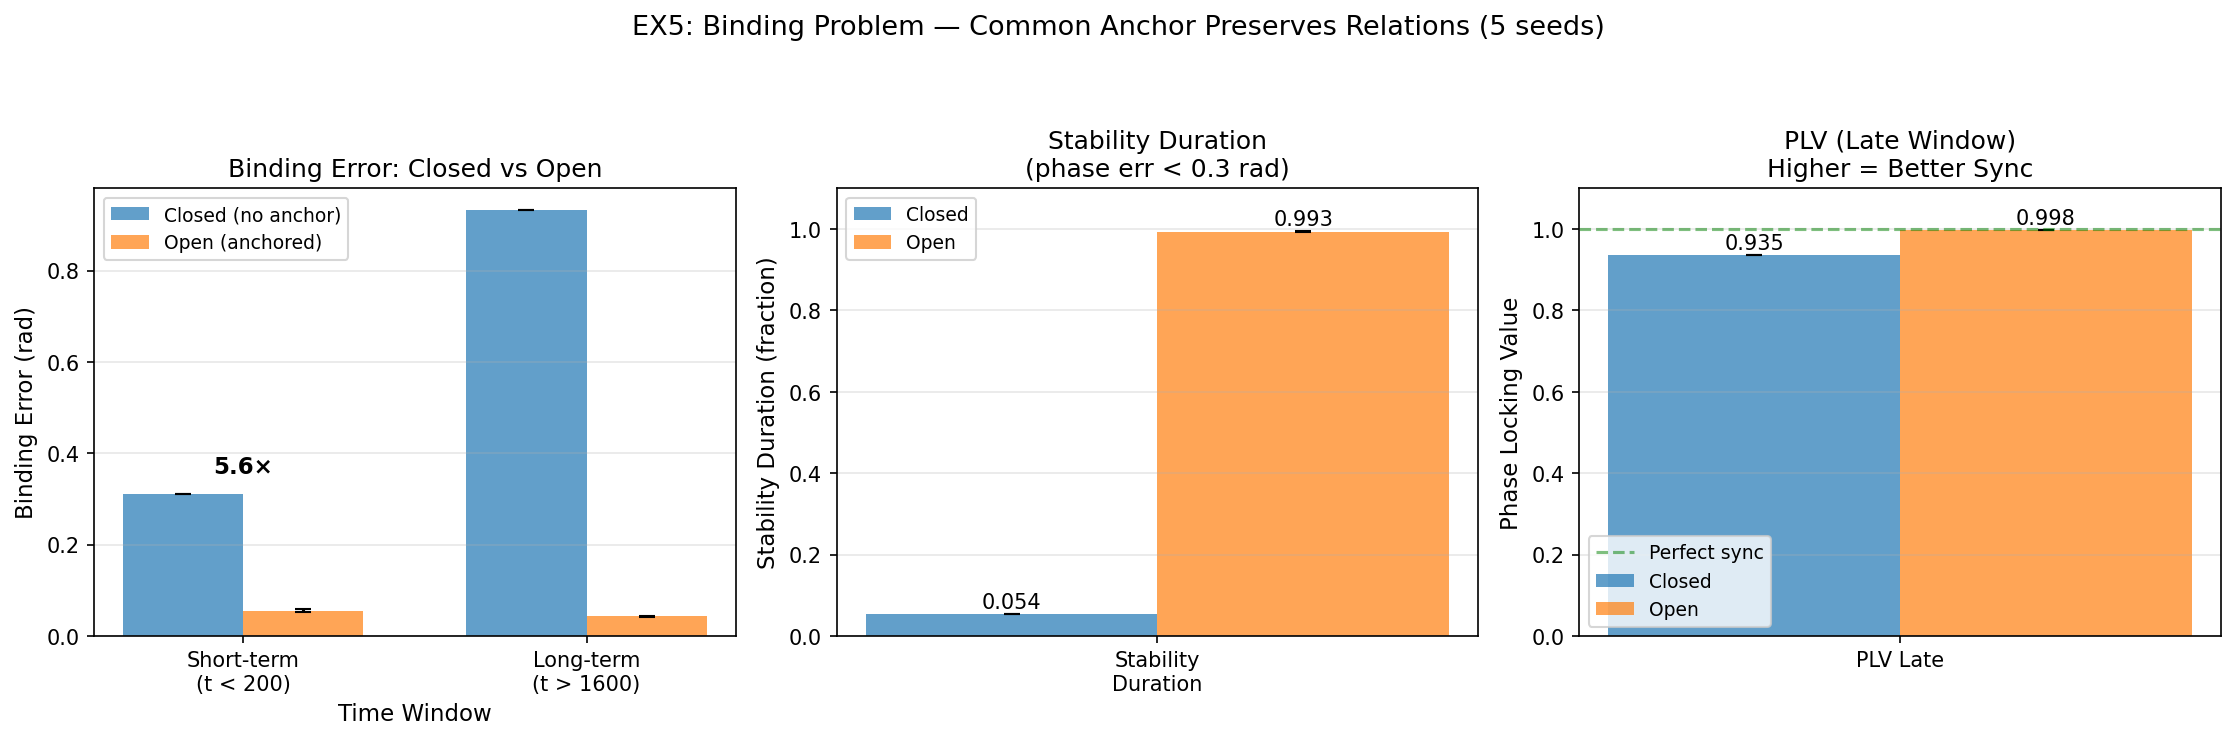
\includegraphics[width=\textwidth]{results_ex5/ex5_aggregate.png}
    \caption{\textbf{EX5 Aggregate Metrics (20 seeds).}
    \textbf{Left:} Binding error (short: $t<200$, long: $t>1600$).
    \textbf{Middle:} Stability duration (fraction of steps with $E_{\mathrm{bind}} < 0.3$ rad).
    \textbf{Right:} Phase-locking value $\mathrm{PLV}_{\mathrm{late}}$.
    The anchored system (Open) preserves relations over long horizons with near-perfect PLV and high stability duration.}
    \label{fig:ex5_aggregate}
\end{figure}

\begin{figure}[t]
    \centering
    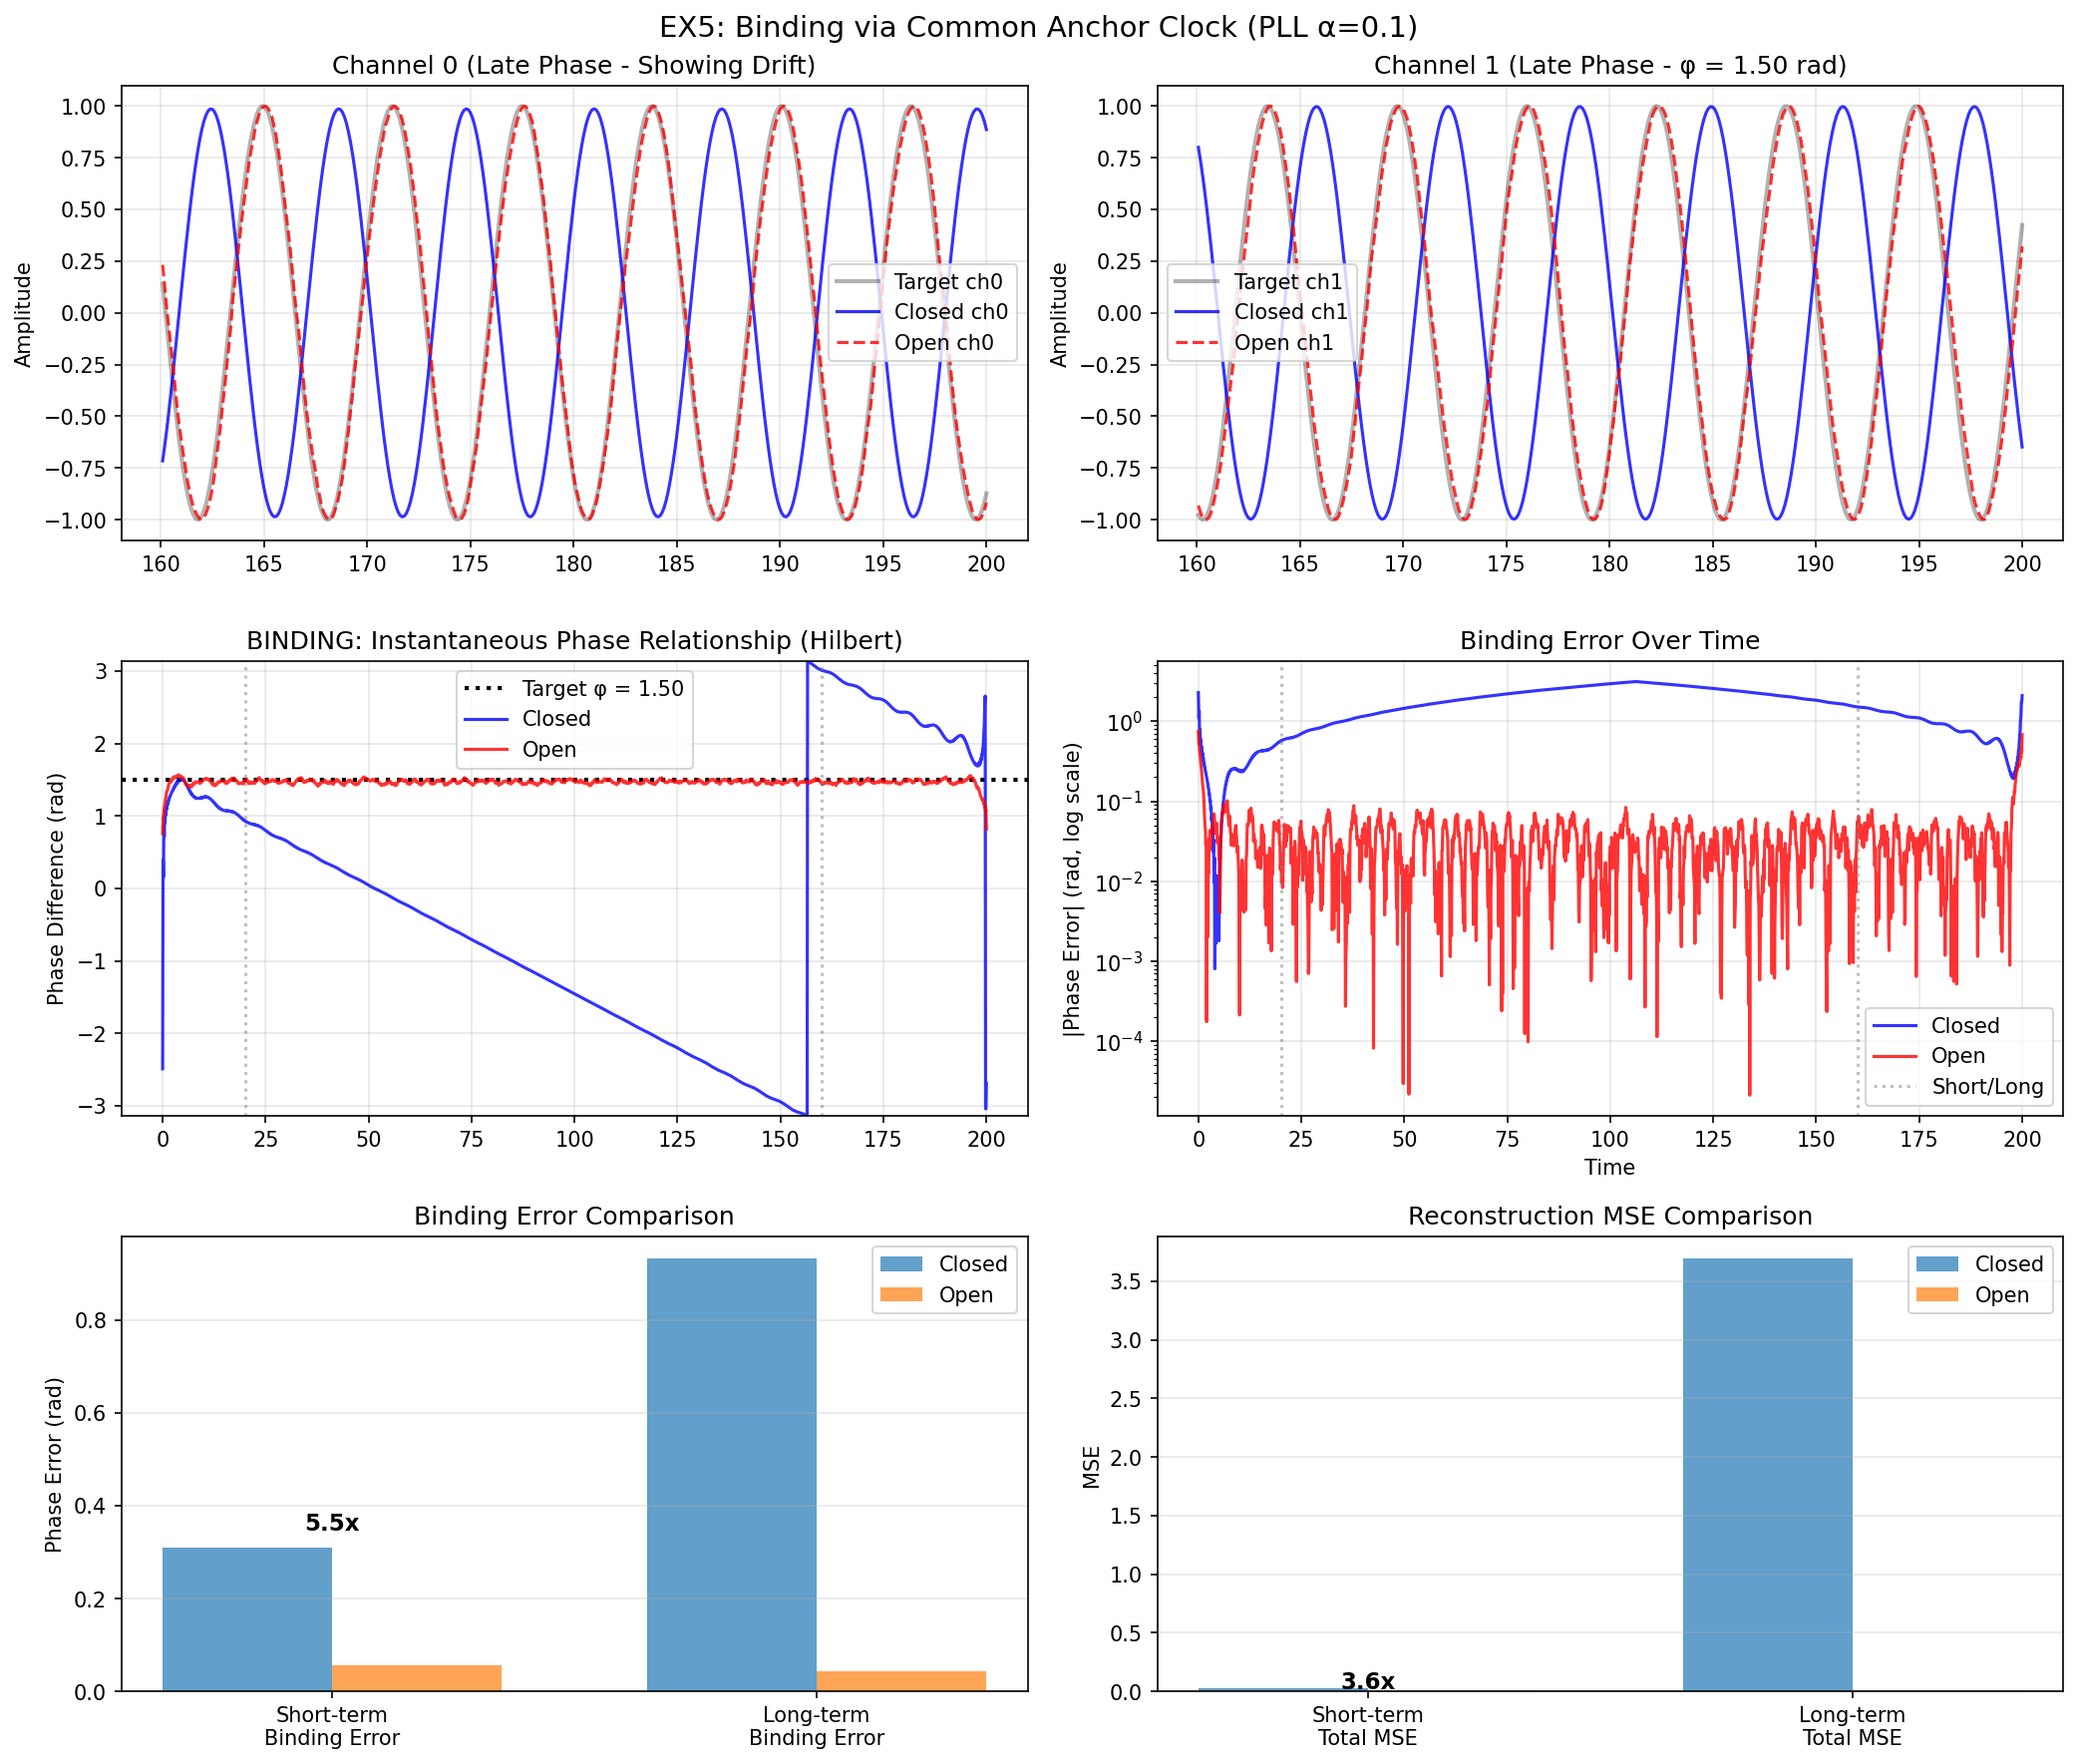
\includegraphics[width=\textwidth]{results_ex5/ex5_binding.png}
    \caption{\textbf{EX5 Detailed Dynamics (Seed=0).}
    \textbf{Top:} Late-phase waveforms showing drift in Closed vs.\ tracking in Open.
    \textbf{Middle:} Instantaneous phase difference (Hilbert) and binding error over time.
    \textbf{Bottom:} Summary comparison of binding error and MSE across time windows.
    Open maintains near-constant relative phase; Closed exhibits systematic drift.}
    \label{fig:ex5_binding_dynamics}
\end{figure}


\clearpage

%%%%%%%%%%%%%%%%%%%%%%%%%%%%%%%%%%%%%%%%%%%%%%%%%%%%%%%%%%%%%%%%%
% EXPERIMENT 6: Frozen-Code Category Recognition
%%%%%%%%%%%%%%%%%%%%%%%%%%%%%%%%%%%%%%%%%%%%%%%%%%%%%%%%%%%%%%%%%
\section{Experiment 6: Frozen-Code Category Recognition}

\subsection{Purpose}
Experiment 6 (EX6) tests whether \emph{new inference} can occur \emph{after learning is stopped}. Here, “inference” refers strictly to test-time routing and reconstruction behavior under frozen parameters (no gradient updates), so any differential response must arise from the existing discrete/gating dynamics rather than further learning. We first train a MultiGate model on a subset of Lissajous categories and then \textbf{freeze the discrete codebook}.
In the frozen phase, the model is exposed to both \emph{trained} shapes and a \emph{withheld} shape (never seen during training).
Because parameters are frozen, any change in behavior must arise from \textbf{internal routing dynamics} rather than gradient-based adaptation.

\subsection{Theoretical Background}
A key claim of CSCT is that \textbf{discrete symbols are not sufficient by themselves}: what matters is the \emph{dynamical rule} that selects and composes symbols under constraints.
To separate ``learning symbols'' from ``using symbols,'' EX6 explicitly \textbf{freezes} the symbol mechanism (the codebook), forcing the system to rely only on \emph{state transitions} and \emph{gate-controlled routing}.
In this regime, the observed generalization is not readily explained by continued parameter learning; instead, the frozen multi-gate dynamics remain sensitive to input geometry, yielding stable routing for familiar inputs and reorganized routing for novel ones.

\paragraph{Convex Hull Constraint (Axiom A2).}
According to Axiom A2 (Constructive Compression), the reconstruction $\hat{x}$ must be expressible as a convex combination of codebook vectors:
\begin{equation}
    \hat{x} = \sum_{k=1}^{K} \alpha_k \cdot c_k, \quad \alpha_k \geq 0, \quad \sum_k \alpha_k = 1
\end{equation}
where $\{c_k\}$ are the frozen codebook entries.
This defines a fixed polytope (convex hull) $\mathcal{P} \subset \mathbb{R}^D$ that bounds all possible reconstructions.
Crucially, with a convex-combination decoder the model is not expected to extrapolate reliably beyond the span of the trained primitives, so reconstruction typically degrades for inputs that fall outside (or far from) that region.

\paragraph{Implications for Novel Categories.}
The withheld ShapeC (3:1 trefoil) has a fundamentally different frequency structure than the trained shapes (1:1 circle, 2:1 figure-8).
Because the codebook was learned exclusively on trained shapes, the convex hull $\mathcal{P}$ is expected to span primarily the subspace of 1:1 and 2:1 trajectories.
The 3:1 trefoil, lying \textbf{outside this convex hull}, should therefore produce high reconstruction error---not as a failure, but as a mathematically principled measure of geometric novelty.

This experiment connects to the MultiGate interpretation:
\begin{itemize}
    \item \textbf{Code signature} (histogram of selected codes) functions as a discrete representation of the input's category.
    \item \textbf{Gate-state vector} (Na$^{+}$, NMDA, $\theta$) acts as a low-dimensional control signature that modulates routing.
    \item \textbf{Equilibrium statistics} (transition rate, dwell time, entropy) quantify whether the system settles into a stable attractor (category reuse) or remains in a compensatory regime (novel category).
\end{itemize}

\subsection{Task Design}
Each input is a 2D Lissajous trajectory sampled as a short sequence $\{(x_t, y_t)\}_{t=1}^{T}$.
We define three shape categories by their frequency ratios:
\begin{itemize}
    \item \textbf{ShapeA (1:1 Circle):} $x = \sin(t)$, $y = \cos(t)$ --- trained.
    \item \textbf{ShapeB (2:1 Figure-8):} $x = \sin(t)$, $y = \cos(2t)$ --- trained.
    \item \textbf{ShapeC (3:1 Trefoil):} $x = \sin(t)$, $y = \cos(3t)$ --- \textbf{withheld}.
\end{itemize}

All shapes include small amplitude/phase perturbations ($\pm 5\%$ amplitude, $\pm 0.1$ rad phase) to ensure within-category variability.
Training uses only ShapeA and ShapeB. After training, the codebook is frozen, and evaluation includes all three shapes.

\subsection{Hypothesis}
We test the following hypotheses under the \emph{frozen-code} regime:
\begin{itemize}
    \item \textbf{H1 (Convex Hull Exclusion):} The withheld ShapeC lies outside the convex hull spanned by the frozen codebook, and is therefore expected to yield substantially higher reconstruction error than trained shapes; this error serves as an operational proxy for geometric novelty relative to the trained subspace.
    \item \textbf{H2 (MSE as Distance Measure):} Reconstruction error (MSE) should be substantially higher for the withheld ShapeC than for trained shapes, providing a robust signal for out-of-distribution detection.
    \item \textbf{H3 (Code Reuse Phenomenon):} Despite lying outside the convex hull, the withheld shape may produce similar code histogram statistics to trained shapes (low JSD difference), because the system projects novel inputs onto familiar basis vectors. This would demonstrate that distributional metrics on codes are unreliable indicators of geometric novelty.
\end{itemize}

\subsection{Method}

\subsubsection{Anchor Configuration}
Self-referential anchor configuration: $y = x$. The Lissajous trajectory serves as its own temporal reference.

\subsubsection{Parameters and Training}
\begin{itemize}
    \item \textbf{Model Parameters:} Architecture = MultiGate, Codebook size $K=16$, hidden dimension $32$, latent dimension $z=2$.
    \item \textbf{Training Configuration:} Training steps $S=2000$ on ShapeA and ShapeB only, sequence length $T=128$, $N=50$ seeds.
    \item \textbf{Frozen Inference:} After training, all parameters are frozen. Evaluation alternates inputs from all three categories.
\end{itemize}

\subsection{Metrics}
\begin{itemize}
    \item \textbf{Jensen-Shannon Divergence (JSD):} Measures distributional distance between code histograms. Within-trained JSD compares ShapeA--ShapeB; to-withheld JSD compares trained shapes to ShapeC. We use Jensen-Shannon divergence $\mathrm{JSD}(p,q)=\tfrac12\mathrm{KL}(p\|m)+\tfrac12\mathrm{KL}(q\|m)$ with $m=\tfrac12(p+q)$ on normalized code-usage histograms (lower is more similar).

    \item \textbf{Clustering Metrics:} Adjusted Rand Index (ARI) and Normalized Mutual Information (NMI) from KMeans ($k=2$: trained vs.\ withheld). ARI/NMI are computed by clustering per-trial feature vectors (histograms or transition-signatures) into $k{=}2$ groups and comparing the assignments against the ground-truth label \{trained vs withheld\}; linear separability reports cross-validated logistic-regression accuracy on the same features.

    \item \textbf{Linear Separability:} Logistic regression accuracy on code histograms, transition features, and gate-state vectors.
    \item \textbf{Reconstruction MSE:} Mean squared error between input and reconstruction.
\end{itemize}

\subsection{Results}

Across $N=50$ independent seeds, the frozen codebook exhibits clear differential behavior between trained shapes (ShapeA, ShapeB) and the withheld shape (ShapeC), primarily through reconstruction error.
Table~\ref{tab:ex6_summary} summarizes the aggregate statistics.

\begin{table}[t]
    \centering
    \caption{Experiment 6 summary (mean $\pm$ std across seeds).}
    \label{tab:ex6_summary}

    % --- Subtable (a): Code Statistics (Distribution, Clustering, Separability) ---
    \begin{subtable}{\columnwidth}
        \centering
        \caption{Code Distribution \& Clustering Metrics}
        \resizebox{\columnwidth}{!}{%
        \begin{tabular}{lcccccc}
            \toprule
            Group & JSD (Within) & JSD (Withheld) & JSD Diff & ARI (Hist) & NMI (Hist) & Linear Sep. \\
            \midrule
            Pooled & $0.277 \pm 0.069$ & $0.253 \pm 0.034$ & $-0.024 \pm 0.048$ & $0.473 \pm 0.450$ & $0.576 \pm 0.359$ & $0.667 \pm 0.000$ \\
            \bottomrule
        \end{tabular}
        }
    \end{subtable}

    \vspace{0.4cm} % Space between tables

    % --- Subtable (b): Reconstruction Metrics (Primary Signal) ---
    \begin{subtable}{\columnwidth}
        \centering
        \caption{Reconstruction Quality (Out-of-Distribution Signal)}
        \resizebox{\columnwidth}{!}{%
        \begin{tabular}{lccc}
            \toprule
            Group & MSE (Trained) & MSE (Withheld) & MSE Ratio (Withheld/Trained) \\
            \midrule
            Pooled & $0.0495 \pm 0.0079$ & $0.1837 \pm 0.0346$ & \textbf{3.79 $\pm$ 0.91} \\
            \bottomrule
        \end{tabular}
        }
    \end{subtable}
\end{table}


\begin{itemize}
    \item \textbf{Reconstruction Quality (Primary Metric).}
    The trained family achieves $\mathrm{MSE} = 0.0495 \pm 0.0079$, while the withheld condition rises to $0.1837 \pm 0.0346$ (ratio $3.79 \pm 0.91$, range 2.37--6.51).
    Notably, \textbf{all 50 seeds} produced MSE ratio $> 2.0$, demonstrating that reconstruction error provides a perfectly reliable signal for detecting novel categories under frozen-codebook conditions.

    \item \textbf{Code Distribution Divergence.}
    The within-trained JSD (ShapeA vs.\ ShapeB) is $0.277 \pm 0.069$, and the to-withheld JSD (trained vs.\ ShapeC) is $0.253 \pm 0.034$.
    The small difference ($\Delta\mathrm{JSD} = -0.024 \pm 0.048$) indicates that code histogram divergence alone does not reliably distinguish withheld shapes from trained ones at this codebook size.

    \item \textbf{Clustering Performance.}
    Unsupervised clustering (KMeans, $k=2$) achieves moderate performance: $\mathrm{ARI} = 0.473 \pm 0.450$ and $\mathrm{NMI} = 0.576 \pm 0.359$ on histogram features.
    Linear separability reaches $0.667$ for histogram, transition, and gate features.
    The high variance across seeds suggests that clustering-based \emph{category detection} (rather than component separation) is seed-dependent.
\end{itemize}

\subsection{Discussion}

EX6 provides evidence that \emph{after learning is stopped}, the frozen multi-gate system can still exhibit differential responses to trained versus withheld categories, while reconstruction quality remains constrained by the fixed codebook.
The key finding is that \textbf{reconstruction error (MSE ratio) provides a robust and computationally efficient signal for out-of-distribution detection}, while code histogram divergence (JSD) fails as a discriminative metric. Accordingly, EX6 should be interpreted as category detection under a frozen codebook (trained vs. withheld), not as component separation or semantic recovery of the withheld category.

\paragraph{Geometric Interpretation via Convex Hull (Axiom A2).}
This result provides direct empirical support for \textbf{Axiom A2 (Constructive Compression in Simplex)}.
Mathematically, the frozen codebook defines a fixed polytope (convex hull) $\mathcal{P} \subset \mathbb{R}^D$.
Here \(D\) denotes the flattened signal dimension, and \(P\) refers to the set of reconstructions realizable by the frozen decoder when driven by convex combinations of the learned code vectors (i.e., the model’s realizable reconstruction manifold under frozen parameters).
The trained trajectories (ShapeA, ShapeB) lie within or near this subspace, resulting in minimal reconstruction error.
In contrast, the withheld ShapeC lies almost entirely \textbf{outside the convex hull} spanned by the trained basis vectors.
Because reconstruction is constrained to a convex combination of learned primitives, the model is not expected to reconstruct the novel geometry of ShapeC accurately when it lies outside the representational span learned during training.
The high reconstruction error is therefore not a failure, but a principled operational measure of mismatch to the frozen codebook’s constructive capacity, consistent with the convex-hull constraint implied by the axioms.
Conversely, the failure of JSD implies that the \emph{projection} of the novel shape onto the simplex distributes probability mass in a way that mimics familiar categories, highlighting the danger of relying solely on internal symbol statistics without physical grounding.

\paragraph{MSE Ratio as Primary Indicator.}
Across all 50 seeds, the MSE ratio exceeded 2.0 (range: 2.37--6.51, mean $3.79 \pm 0.91$), achieving \textbf{100\% detection rate} under this threshold.
This robustness is consistent with the fact that reconstruction error tends to increase when inputs fall outside the learned representational span, regardless of which discrete codes are selected.

\paragraph{Why JSD Failed.}
In contrast, code histogram divergence ($\Delta\mathrm{JSD} = -0.024 \pm 0.048$) failed to distinguish withheld from trained categories.
This failure reflects a \textbf{codebook reuse} phenomenon: faced with an unfamiliar input, the frozen system does not allocate ``new'' codes (which do not exist) but instead \emph{repurposes existing codes suboptimally}.
The resulting histogram may be statistically similar to trained distributions---or even closer, as the system attempts to approximate the novel shape using familiar building blocks---yet the reconstruction quality degrades substantially.
This decoupling between code selection patterns and reconstruction fidelity explains why distributional metrics on discrete codes are unreliable for out-of-distribution detection in frozen-codebook settings.

\paragraph{Computational and Extensibility Advantages of MSE.}
Beyond robustness, MSE-based detection offers significant practical advantages for future extensions:
\begin{itemize}
    \item \textbf{Computational efficiency:} MSE is a single scalar computed from the reconstruction, requiring $O(T \cdot d)$ operations for sequence length $T$ and dimension $d$. In contrast, JSD requires maintaining and comparing $K$-dimensional histograms, with complexity scaling as $O(T + K)$ per comparison and $O(K^2)$ for pairwise category comparisons.
    \item \textbf{Scalability:} As codebook size $K$ increases or multiple codebooks are employed (e.g., hierarchical VQ), histogram-based metrics become increasingly expensive and statistically noisy. MSE remains invariant to codebook structure.
    \item \textbf{Online applicability:} MSE can be computed incrementally during inference, enabling real-time anomaly detection. Histogram-based metrics require accumulating statistics over complete sequences before comparison.
\end{itemize}

\paragraph{Implications for CSCT.}
These results suggest that the ``meaning'' of discrete codes in a frozen system is best assessed through their \emph{downstream functional consequences} (reconstruction quality) rather than their \emph{distributional statistics} (histogram similarity).
This aligns with CSCT's emphasis on grounded symbol interpretation: symbols acquire meaning through their causal role in generating behavior, not through abstract distributional properties.
The convex hull constraint (Axiom A2) ensures that the system's representational capacity is bounded and interpretable, with reconstruction error serving as a principled measure of geometric novelty.

\subsection{Visual Analysis}

Figure \ref{fig:ex6_aggregate} reveals a critical dissociation between symbolic statistics and physical grounding. While distributional metrics (JSD) often fail to distinguish the withheld category due to code reuse, the reconstruction MSE provides a decisive detection signal, yielding an error approximately $3.79\times$ higher than trained categories. Figure \ref{fig:ex6_reconstruction} visualizes the mechanism behind this "Ungrounded Symbol Acquisition." Trained shapes (Left/Center) exhibit stable, phase-locked reconstruction within the learned convex hull. Conversely, the withheld shape (Right) triggers erratic approximations; the system forces a discrete interpretation using existing codes, but the lack of geometric support results in a physically incoherent trajectory. This visual contrast validates that valid cognition requires not just symbol generation, but containment within the convex hull (Axiom A2).

% --- Figure 1: Aggregate Statistics ---
\begin{figure}[t]
    \centering
    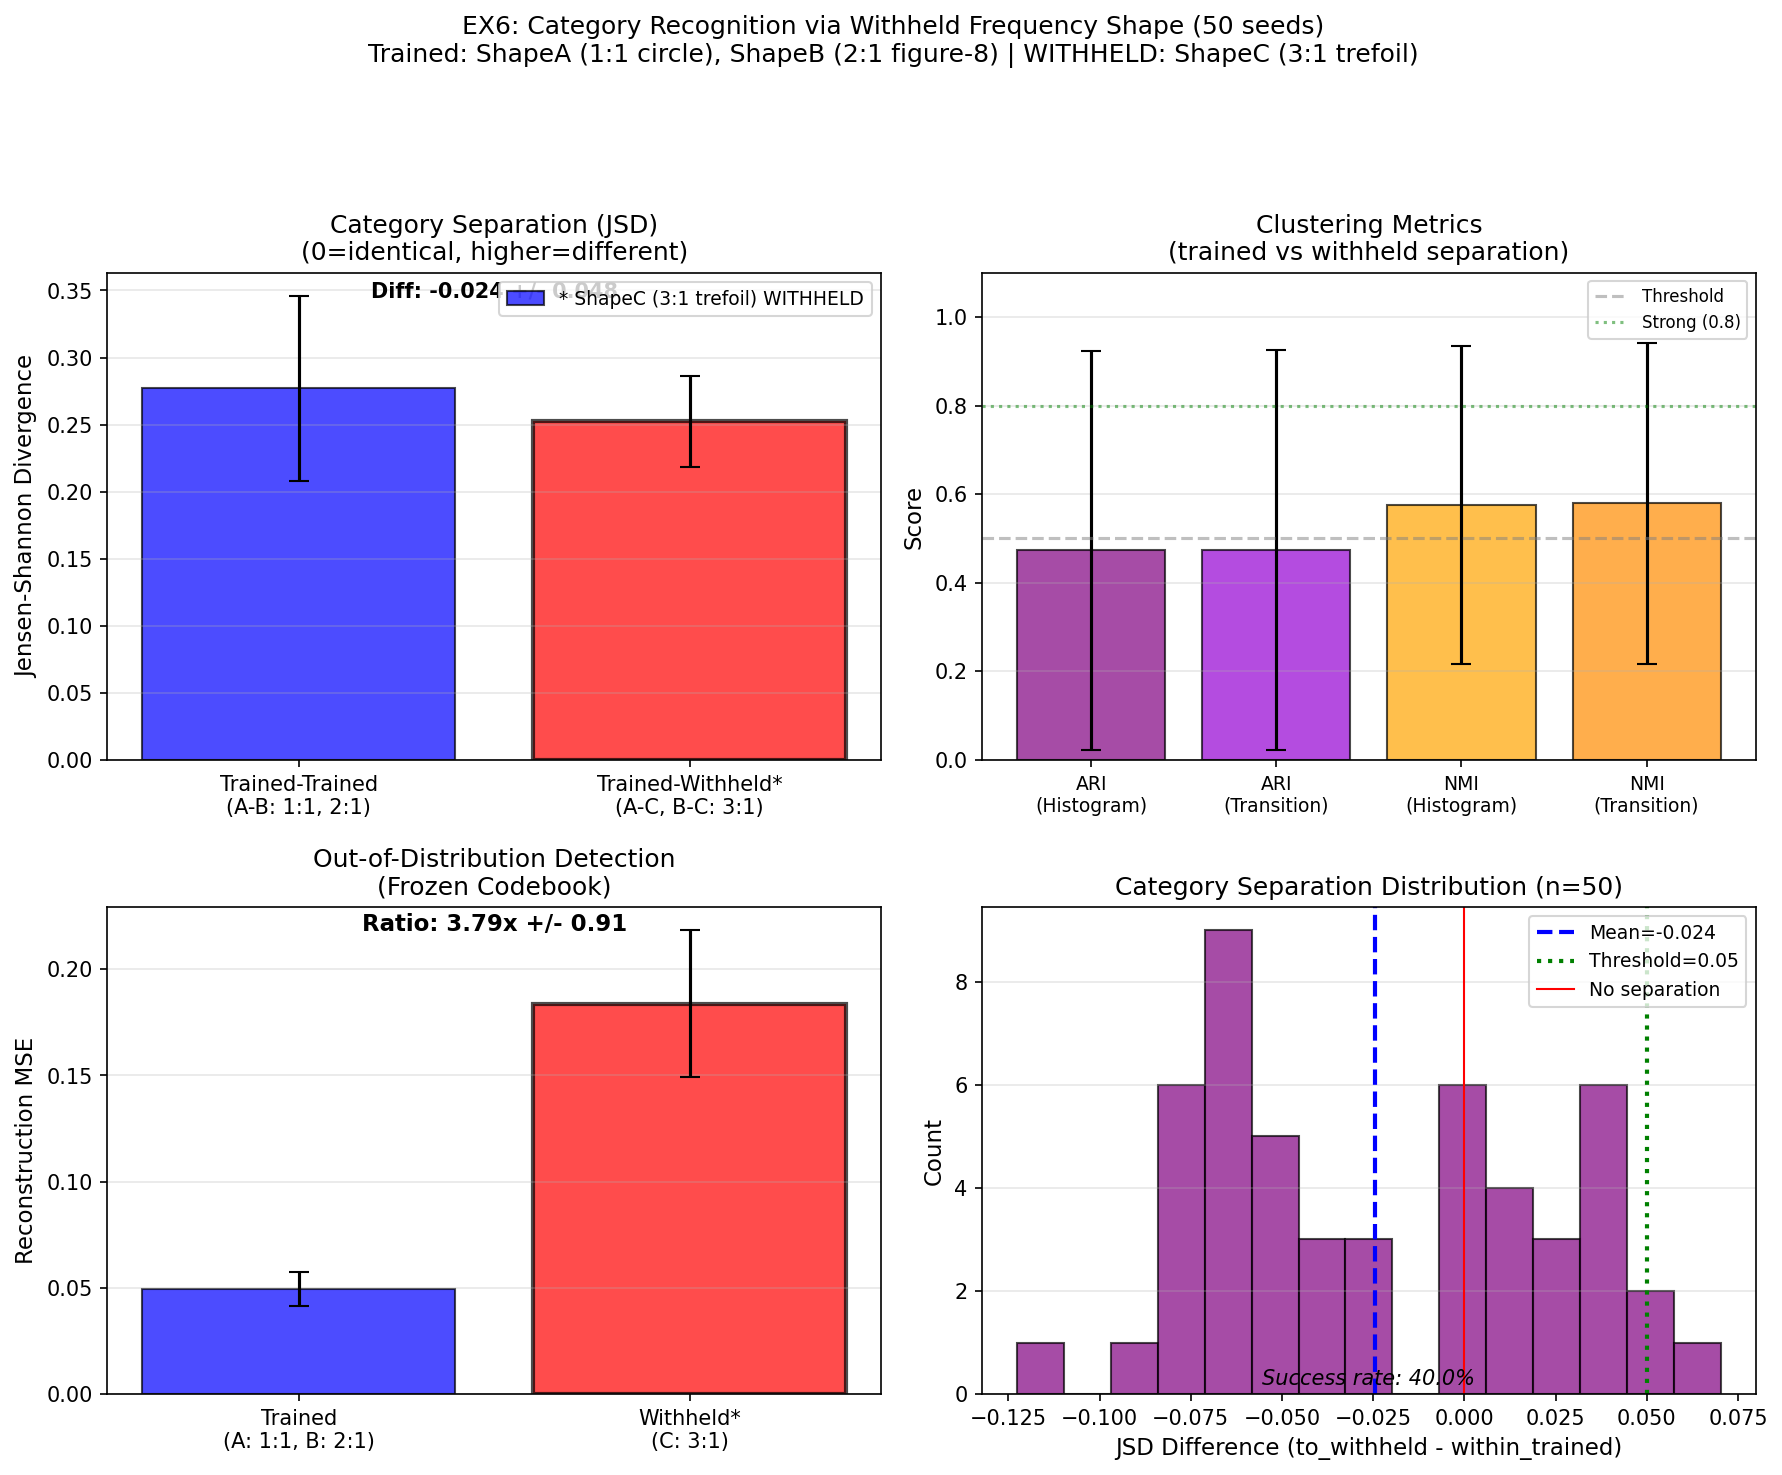
\includegraphics[width=1.0\linewidth]{results_ex6/ex6_aggregate.png}
    \caption{\textbf{EX6 Aggregate Statistics (50 seeds).}
    Top-left: JSD between trained and withheld categories.
    Top-right: Clustering metrics (ARI, NMI).
    Bottom-left: Reconstruction MSE ratio.
    Bottom-right: JSD difference distribution.
    These metrics summarize the distributional behavior of the frozen codebook.}
    \label{fig:ex6_aggregate}
\end{figure}

% --- Figure 2: Representative Reconstructions ---
\begin{figure}[t]
    \centering
    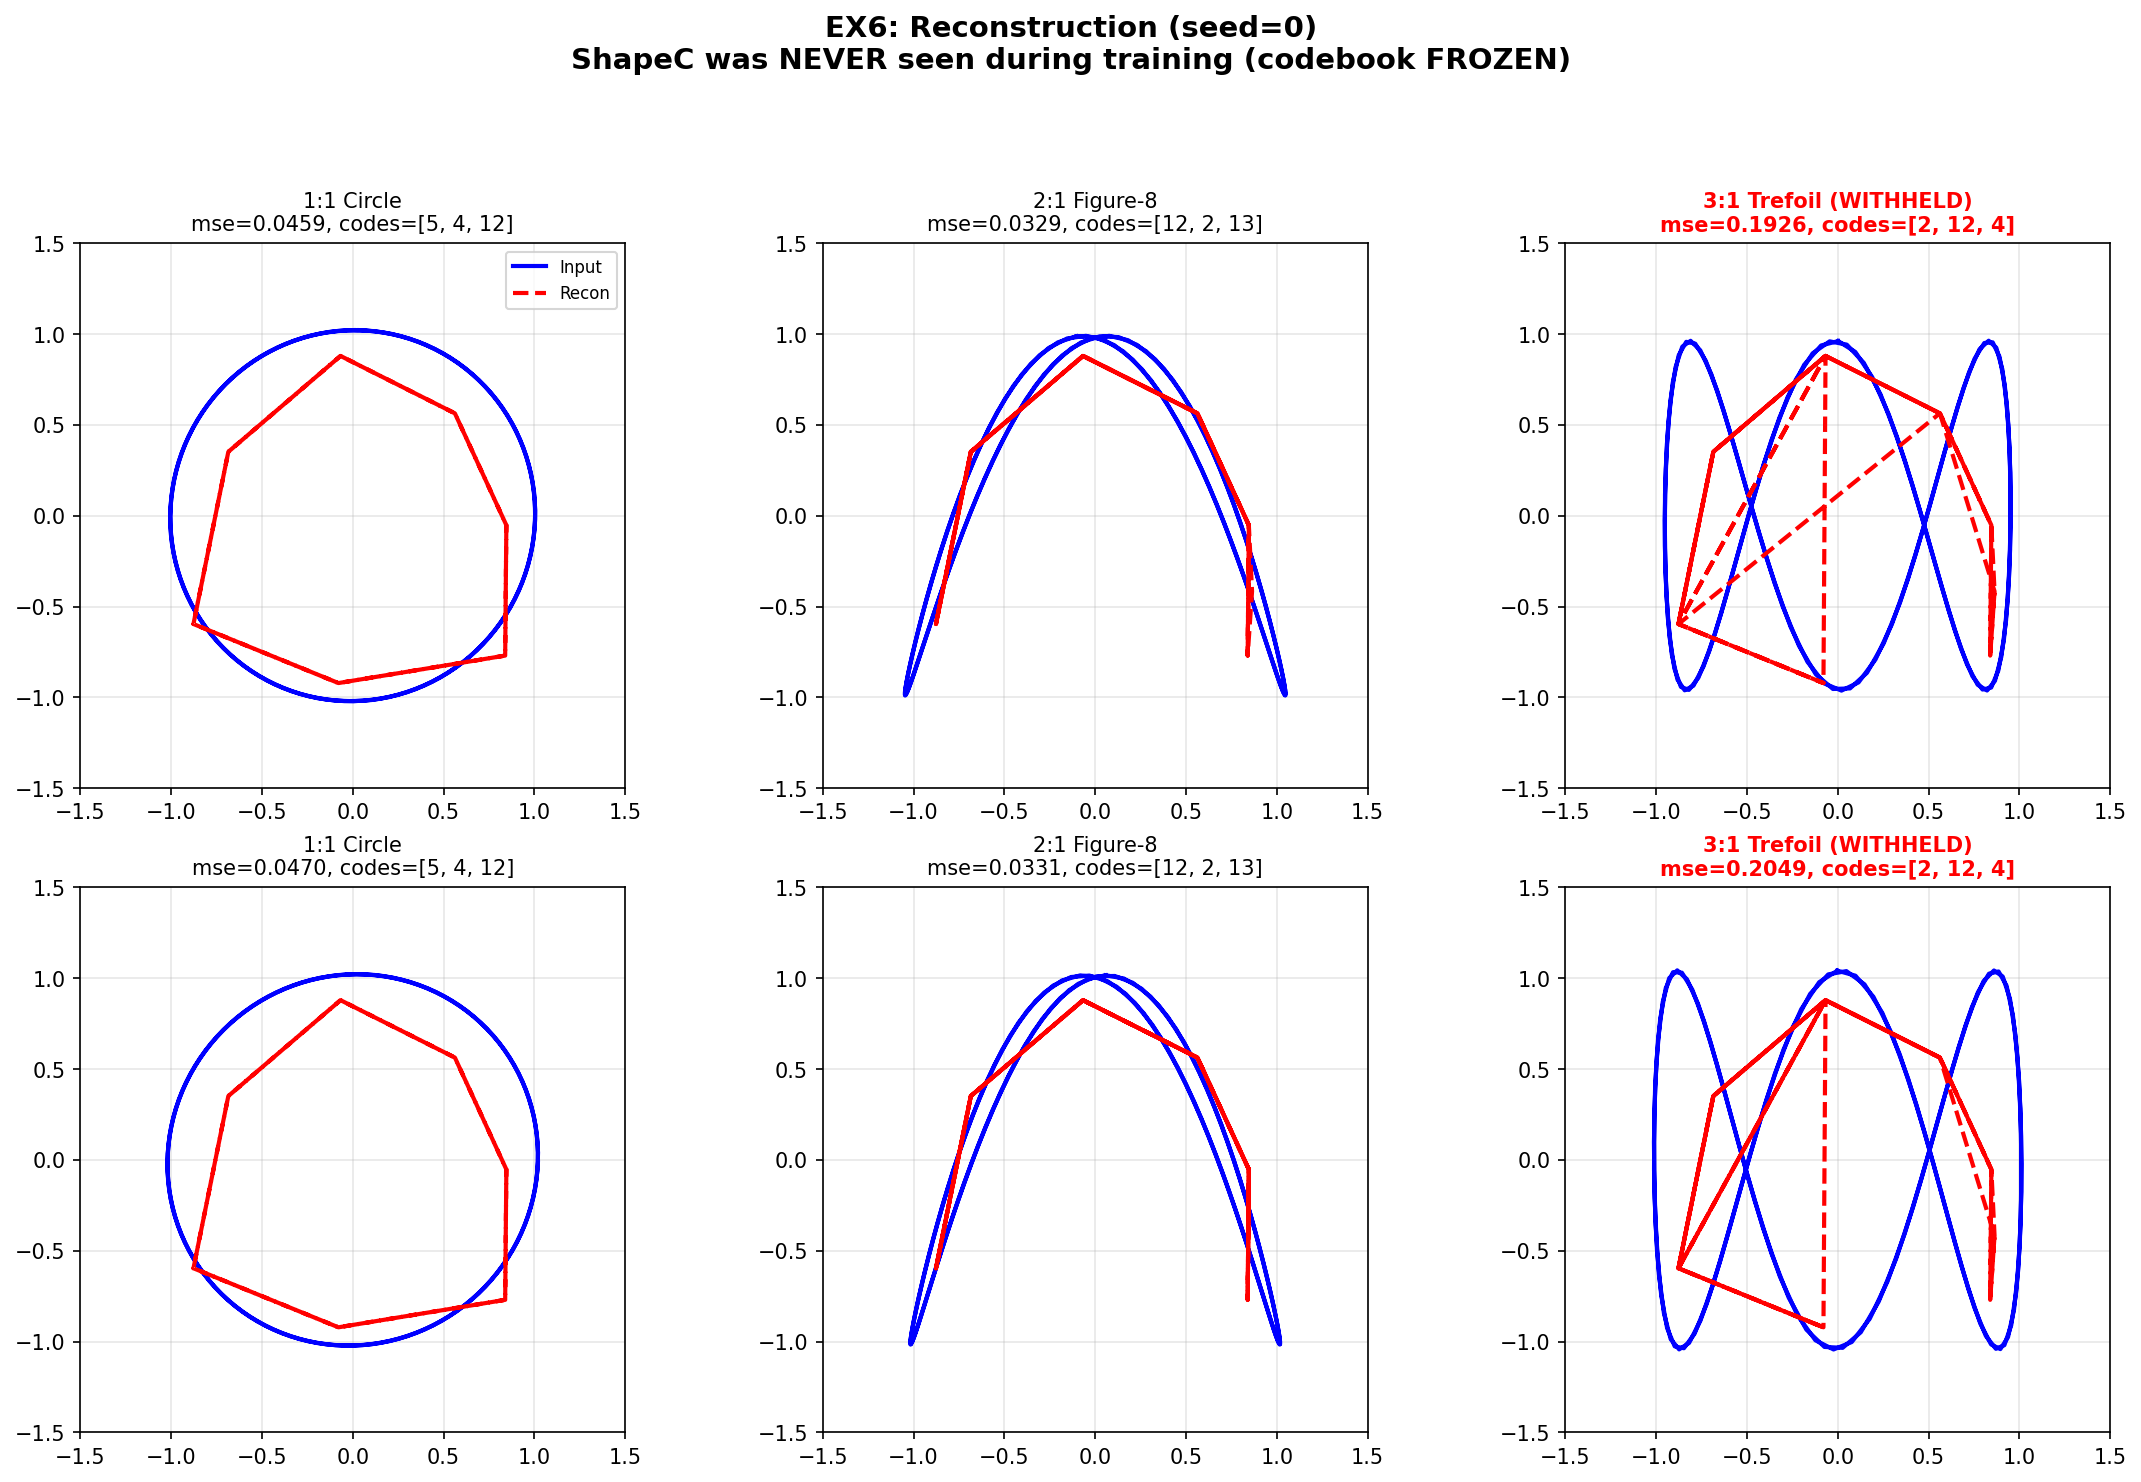
\includegraphics[width=1.0\linewidth]{results_ex6/ex6_reconstruction.png}
    \caption{\textbf{EX6 Representative Reconstructions (Seed=0).}
    Comparison of input trajectory (blue) and frozen-codebook reconstruction (red).
    \textbf{Left/Center:} Trained shapes (ShapeA, ShapeB) are reconstructed with high fidelity.
    \textbf{Right:} The withheld ShapeC (3:1 trefoil) triggers different code usage and significantly higher MSE, serving as a geometric signal for OOD detection.}
    \label{fig:ex6_reconstruction}
\end{figure}

\clearpage

%%%%%%%%%%%%%%%%%%%%%%%%%%%%%%%%%%%%%%%%%%%%%%%%%%%%%%%%%%%%%%%%%
% EXPERIMENT 7: Relational Internal Time
%%%%%%%%%%%%%%%%%%%%%%%%%%%%%%%%%%%%%%%%%%%%%%%%%%%%%%%%%%%%%%%%%
\section{Experiment 7: Relational Internal Time}

\subsection{Purpose}
Experiment 7 (EX7) examines whether internal time (measured as discrete code transition rate) scales with external anchor tempo. This tests a key prediction of CSCT: that internal ``subjective time'' is not an absolute clock but is driven by external signal dynamics.

\subsection{Task Design}
If a signal changes rapidly, the system should process more state transitions per unit of physical time; if the signal is static, internal time should effectively stop.

The experimental design uses a ``train-once, deploy-many'' paradigm:
\begin{itemize}
    \item \textbf{Training Phase:} The model is trained on a ``Standard World'' signal with base frequency $f_0 = 0.5$ Hz. The model learns a codebook and transition dynamics appropriate for this tempo.
    \item \textbf{Deployment Phase:} The trained model (with frozen weights) is tested on four different ``worlds'' that vary only in temporal scaling:
    \begin{enumerate}
        \item \textbf{Standard World:} Same as training, $f = 0.5$ Hz. Baseline condition.
        \item \textbf{Fast World:} Signal is time-compressed (frequency increases from $0.5 \to 1.5$ Hz). The same waveform shape plays at $3\times$ speed.
        \item \textbf{Slow World:} Signal is time-dilated (frequency decreases from $0.5 \to 0.15$ Hz). The same waveform shape plays at $\sim 0.3\times$ speed.
        \item \textbf{Null World:} Zero input (no signal). Tests whether internal dynamics halt without external drive.
    \end{enumerate}
\end{itemize}

The key measure is the \textit{transition rate}: how many discrete code changes occur per unit of physical time. If CSCT's internal time is flux-driven, the Fast world should show higher transition rates and the Slow world lower rates, while the Null world should show near-zero transitions. Critically, the \textit{representational content} (which codes are used) should remain invariant---only the \textit{rate} of processing should change.

\subsection{Hypothesis}
\begin{itemize}
    \item \textbf{H1 (Fast Acceleration):} Fast world $\Rightarrow$ higher transition rate than Standard.
    \item \textbf{H2 (Slow Dilation):} Slow world $\Rightarrow$ lower transition rate than Standard.
    \item \textbf{H3 (Null Halt):} Null world $\Rightarrow$ near-zero transitions (internal time stops).
    \item \textbf{H4 (Content Invariance):} The set of unique codes used should remain constant across non-null worlds.
\end{itemize}

\subsection{Method}

\subsubsection{Anchor Configuration}
Self-referential anchor with tempo-warped signals:
\begin{equation}
    x(t) = \frac{\sin(\phi(t)) + 0.5\sin(2\phi(t) + 1.0)}{\max|\sin(\phi(t)) + 0.5\sin(2\phi(t) + 1.0)|}
\end{equation}
where $\phi(t) = \int_0^t 2\pi f(\tau) d\tau$ is the instantaneous phase determined by the frequency profile $f(t)$.

\subsubsection{Parameters and Training}
\begin{itemize}
    \item \textbf{Model Parameters:} Architecture = SingleGate, Codebook size $K=4$, hidden dimension $d=32$, input dimension $D=1$.
    \item \textbf{Training Configuration:} Training epochs $N_{\text{epochs}}=500$, learning rate $\eta=0.01$, sequence length $T=800$, $N=20$ seeds.
    \item \textbf{Frequency Profiles:} Standard: $0.5$ Hz constant; Fast: $0.5 \to 1.5$ Hz; Slow: $0.5 \to 0.15$ Hz; Null: $0$ Hz.
\end{itemize}

\subsection{Metrics}
\begin{itemize}
    \item \textbf{Number of Transitions:}
    \begin{equation}
        N_{\text{trans}} = \sum_{t=1}^{T-1} \mathbf{1}[s_t \neq s_{t-1}]
    \end{equation}
    \item \textbf{Transition Rate:}
    \begin{equation}
        r_{\text{trans}} = \frac{N_{\text{trans}}}{T_{\text{physical}}}
    \end{equation}
    \item \textbf{Unique Codes:} Number of distinct code indices used during deployment.
\end{itemize}

\subsection{Results}

Table~\ref{tab:ex7} summarizes the effect of environmental speed on the internal dynamics of the model (mean $\pm$ std across $N=20$ seeds).

\begin{table}[t]
    \centering
    \caption{Experiment 7 summary by world (mean $\pm$ std across seeds).}
    \label{tab:ex7}

    % --- Subtable (a): Frequency Specifications ---
    \begin{subtable}{\columnwidth}
        \centering
        \caption{Frequency Specifications}
        \begin{tabular}{lcccc}
            \toprule
            World & $f_{\min}$ & $f_{\max}$ & $N_{\mathrm{clocks}}$ & $f_0$ \\
            \midrule
            fast & $0.500 \pm 0.000$ & $1.500 \pm 0.000$ & $4 \pm 0$ & $0.500 \pm 0.000$ \\
            slow & $0.151 \pm 0.000$ & $0.500 \pm 0.000$ & $4 \pm 0$ & $0.500 \pm 0.000$ \\
            standard & $0.500 \pm 0.000$ & $0.500 \pm 0.000$ & $4 \pm 0$ & $0.500 \pm 0.000$ \\
            NULL & $0.000 \pm 0.000$ & $0.000 \pm 0.000$ & $4 \pm 0$ & $0.500 \pm 0.000$ \\
            \bottomrule
        \end{tabular}
    \end{subtable}

    \vspace{0.4cm} % Space between tables

    % --- Subtable (b): Discretization Dynamics ---
    \begin{subtable}{\columnwidth}
        \centering
        \caption{Discretization Dynamics}
        \begin{tabular}{lccc}
            \toprule
            World & Unique codes & Transitions & Trans./sec \\
            \midrule
            fast & $4.00 \pm 0.00$ & $90.2 \pm 9.9$ & $4.513 \pm 0.493$ \\
            slow & $4.00 \pm 0.00$ & $29.3 \pm 3.3$ & $1.465 \pm 0.165$ \\
            standard & $4.00 \pm 0.00$ & $56.4 \pm 11.5$ & $2.820 \pm 0.575$ \\
            NULL & $1.00 \pm 0.00$ & $0.0 \pm 0.0$ & $0.000 \pm 0.000$ \\
            \bottomrule
        \end{tabular}
    \end{subtable}
\end{table}


\begin{itemize}
    \item \textbf{Adaptation of Subjective Time (H1--H3).}
    The internal transition rate scales monotonically with external tempo:
    Fast $= 4.513 \pm 0.493$ trans/s (95\% CI [4.291, 4.734]),
    Standard $= 2.820 \pm 0.575$ trans/s (95\% CI [2.561, 3.079]),
    Slow $= 1.465 \pm 0.165$ trans/s (95\% CI [1.391, 1.539]).
    In the Null world (input $= 0$, anchor $= 0$), internal time halts completely: $r_{\text{trans}} = 0.000$, $N_{\text{trans}} = 0$.

    \item \textbf{Invariance of Representation (H4).}
    Despite large changes in transition count (Fast $N_{\text{trans}} = 90.2$, Standard $56.4$, Slow $29.3$), the representational alphabet remains invariant across non-null worlds: unique codes $= 4.00$ (95\% CI [4.00, 4.00]).
    In the Null world, the system freezes into a single state (unique codes $= 1.00$).

    \item \textbf{Dilation Factors.}
    Relative to Standard, Fast shows $1.60\times$ acceleration and Slow shows $0.52\times$ dilation, consistent with the $3\times$ and $0.3\times$ tempo scaling factors.
\end{itemize}

\subsection{Discussion}

EX7 provides strong evidence for the ``Time-Invariance'' property of CSCT representations and the flux-driven nature of internal time (Axiom A4).

\paragraph{Separation of Content and Duration.}
Standard neural networks (e.g., RNNs) often struggle to recognize the same pattern played at different speeds because they sample time absolutely. In contrast, CSCT demonstrates a clear separation: the \textit{content} of the experience (the sequence of 4 codes) is invariant, while the \textit{duration} (the transition rate) absorbs the temporal scaling. This implies that the system recognizes a ``slow wave'' and a ``fast wave'' as the same semantic object, differing only in intensity.

\paragraph{Flux-Driven Cognitive Clock (Axiom A4).}
The scaling of the transition rate ($1.47 \to 4.51$ trans/s) confirms that the ``cognitive clock'' in CSCT is flux-driven. The system does not process ``time''; it processes ``change.'' When the world stops changing (velocity $\to 0$), the internal clock effectively stops. This is biologically consistent with efficient coding principles---resources are expended only when information is actually changing---and creates a form of ``cognitive relativity'' where subjective time depends on the observer's interaction with the environment.

\paragraph{Implications for Temporal Generalization.}
The invariance of the code alphabet across tempo conditions suggests that CSCT representations are inherently tempo-invariant, enabling generalization across temporal scales without retraining. This has practical implications for applications requiring recognition of time-warped signals (e.g., speech at different rates, video at different frame rates).

\subsection{Visual Analysis}

Figure~\ref{fig:ex7_main} presents aggregate statistics across seeds and detailed dynamics for a representative run.

\begin{figure}[t]
    \centering
    \begin{minipage}{1.0\textwidth}
        \centering
        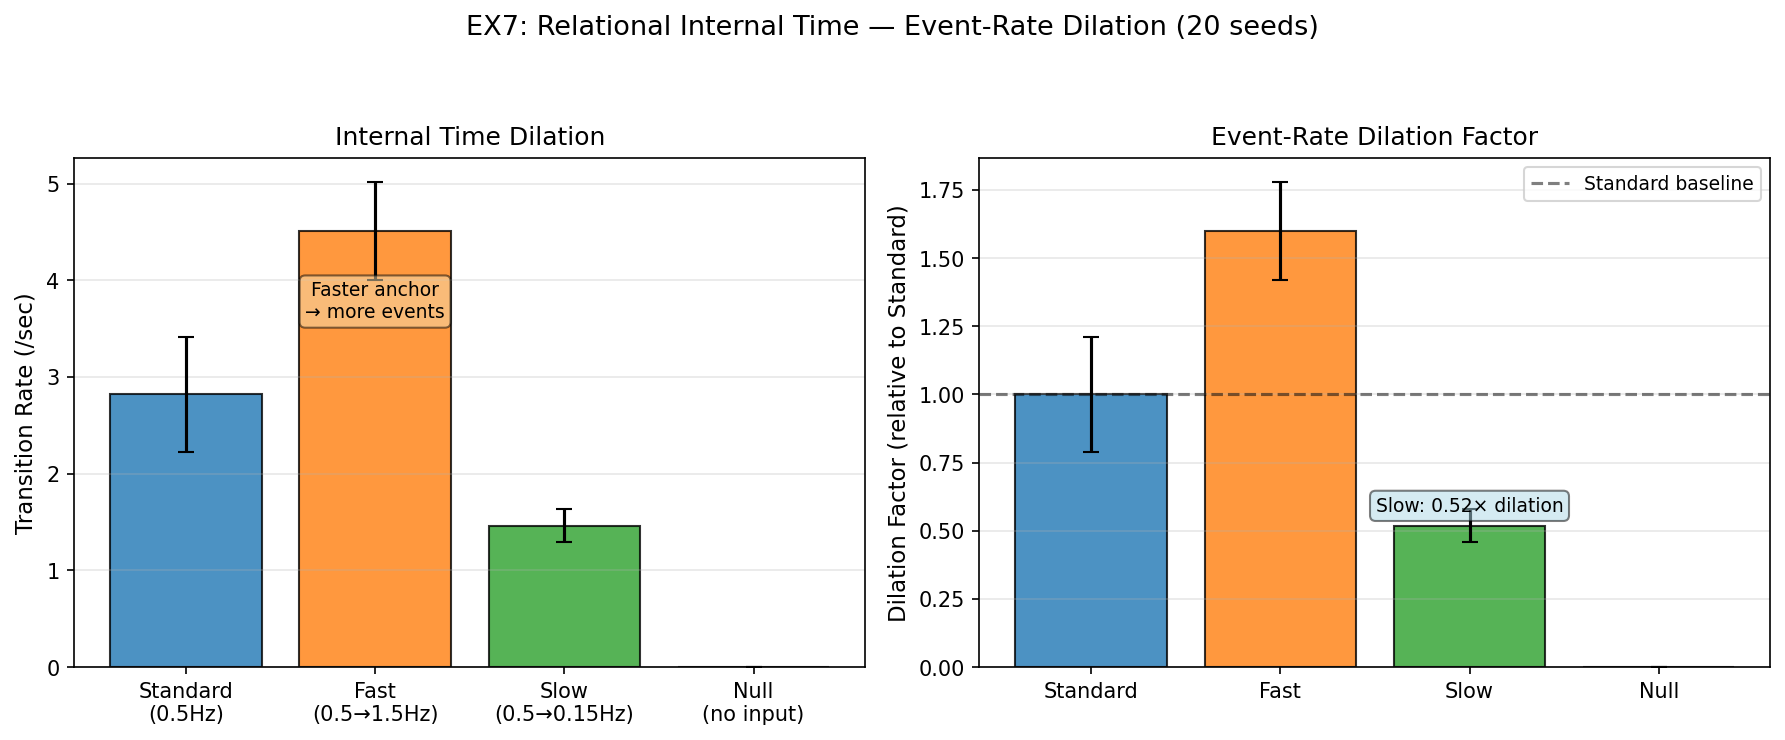
\includegraphics[width=\textwidth]{results_ex7/ex7_aggregate.png}
        \subcaption{\textbf{Aggregate Internal Time Dilation (20 seeds).}
        \textbf{Left:} Mean transition rate (trans/s) under tempo-warp deployment.
        Internal event-rate increases monotonically with environmental tempo (Slow $<$ Standard $<$ Fast), while Null yields zero transitions.
        \textbf{Right:} Dilation factor relative to Standard baseline.
        Error bars indicate mean $\pm$ std across seeds.}
        \label{fig:ex7_aggregate}
    \end{minipage}
    
    \vspace{0.5cm}
    
    \begin{minipage}{1.0\textwidth}
        \centering
        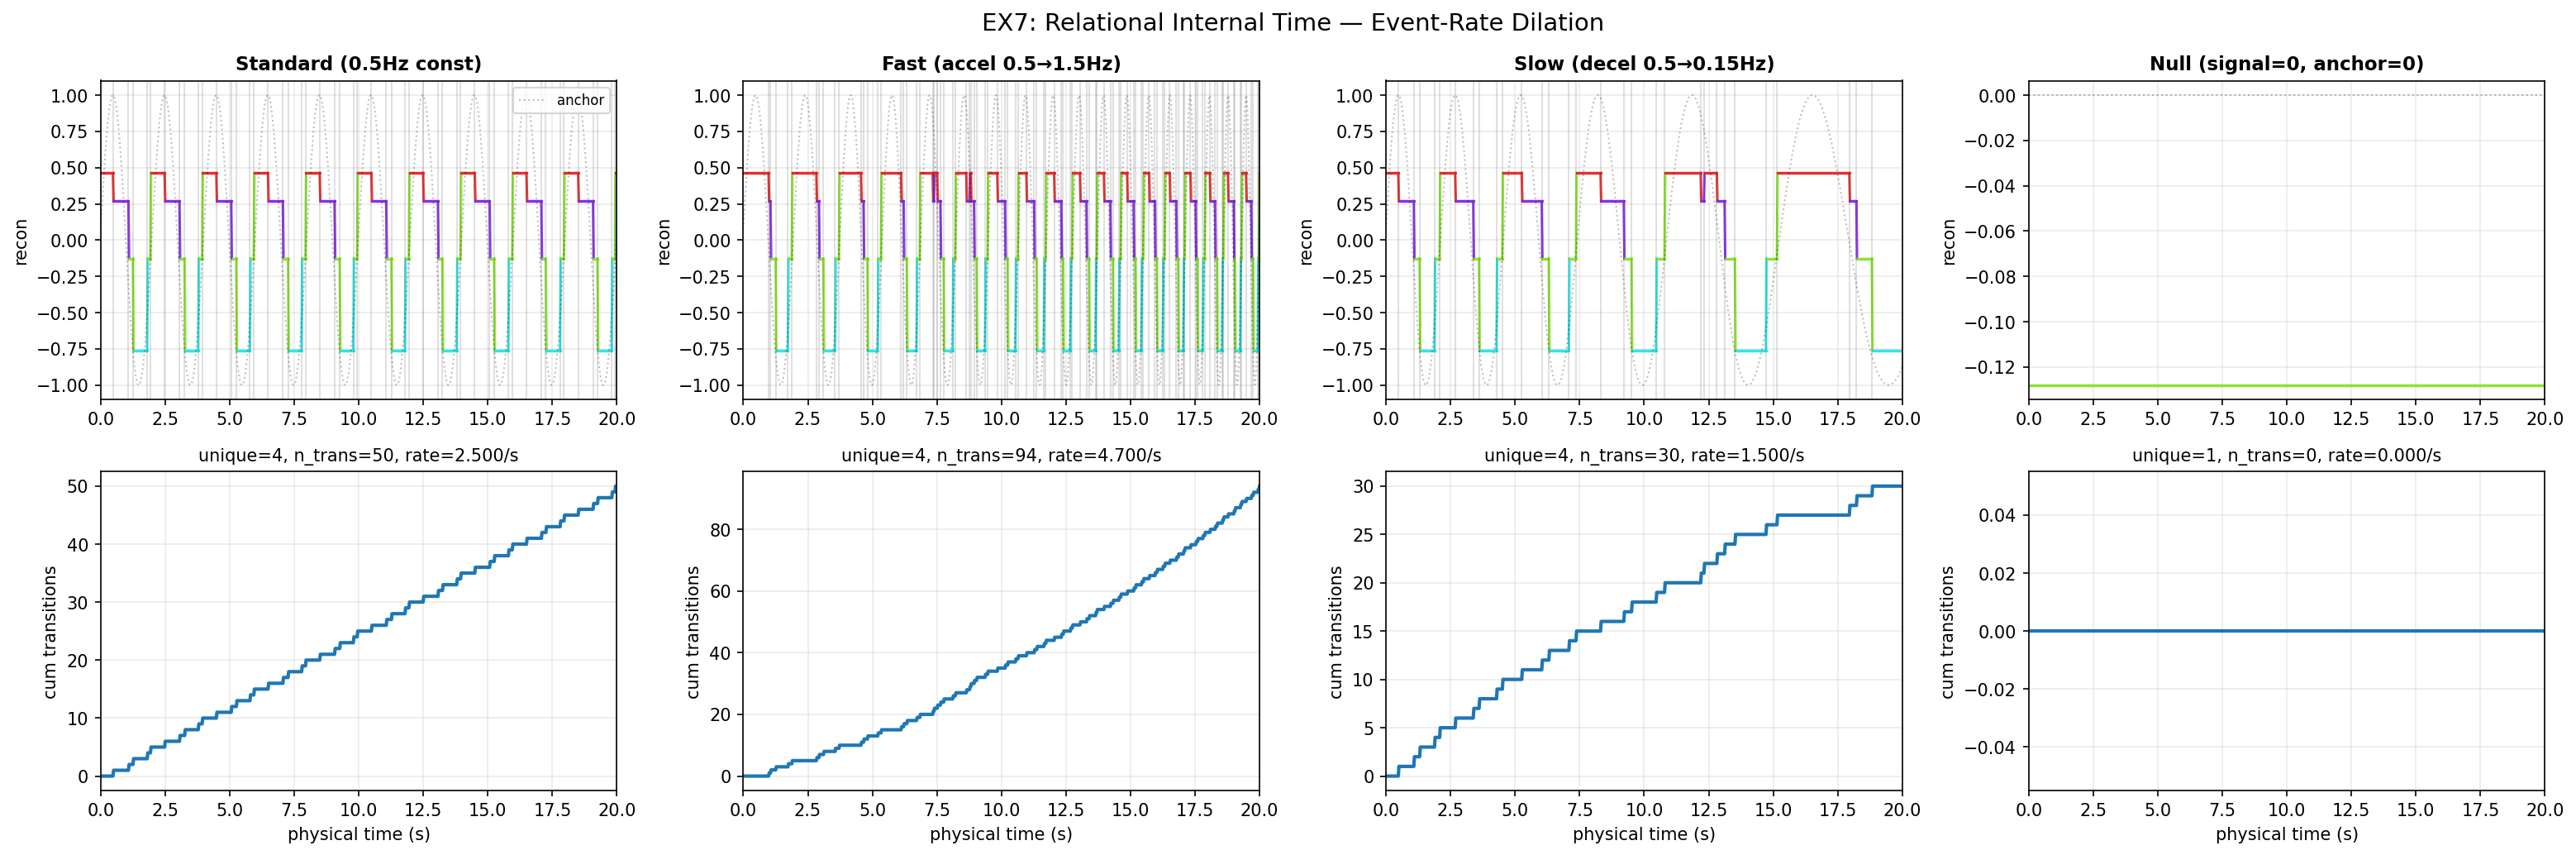
\includegraphics[width=\textwidth]{results_ex7/ex7_relational_time.png}
        \subcaption{\textbf{Single-Seed Dynamics (Seed=0).}
        \textbf{Top:} Reconstructed signal (colored by code) overlaid with anchor waveform (gray dotted).
        \textbf{Bottom:} Cumulative code transitions over physical time.
        The representational alphabet remains stable (4 codes in non-null worlds), while transition rate dilates with tempo; Null freezes ($N_{\text{trans}} = 0$).}
        \label{fig:ex7_single}
    \end{minipage}
    
    \caption{\textbf{EX7: Relational Internal Time---Event-Rate Dilation.}
    A model trained in Standard world ($f_0 = 0.5$ Hz) is deployed with frozen weights to tempo-warped worlds.
    The transition rate of the discrete code sequence serves as an operational measure of internal time velocity.
    Internal time accelerates in faster environments and dilates in slower ones, while Null halts transitions, supporting the relational (flux-driven) nature of time in CSCT.}
    \label{fig:ex7_main}
\end{figure}

\clearpage

%%%%%%%%%%%%%%%%%%%%%%%%%%%%%%%%%%%%%%%%%%%%%%%%%%%%%%%%%%%%%%%%%
% EXPERIMENT 8: Semantic Grounding via Convex Hull
%%%%%%%%%%%%%%%%%%%%%%%%%%%%%%%%%%%%%%%%%%%%%%%%%%%%%%%%%%%%%%%%%
\section{Experiment 8: Semantic Grounding via Convex Hull}

\subsection{Purpose}
Experiment 8 (EX8) investigates the emergence of \emph{semantic grounding} through anchor-driven discrete code learning.
We demonstrate that meaningful token-gate correspondences emerge naturally when the system is trained to separate mixed signals using separated components as anchors.
This experiment provides empirical support consistent with Axiom A2 (Constructive Compression): semantic grounding requires geometric compatibility within the learned simplex.

\subsection{Theoretical Background}
The ``meaning'' of a discrete symbol in CSCT is not defined by its internal structure, but by its relationship to the external world via the anchor.
This is a fundamental departure from purely statistical approaches where tokens emerge from co-occurrence patterns without grounding.

In signal separation, we have a concrete instance of this principle:
\begin{itemize}
    \item A mixture signal $x(t) = \alpha(t) \cdot s_A(t) + \beta(t) \cdot s_B(t)$ contains two sources.
    \item Without access to the separated sources, any decomposition is semantically arbitrary.
    \item By providing separated sources as anchors, we establish ground truth for what each code \emph{should mean}.
\end{itemize}

The key insight is that the anchor breaks the symmetry that would otherwise make the separation task ill-posed.

\paragraph{Convex Hull Constraint (Axiom A2).}
Building on EX6's convex hull analysis, EX8 tests whether a \textbf{withheld primitive} $C$ can be inferred after codebook freezing.
If $C$ lies \emph{inside} the convex hull of the trained primitives, withheld recovery is expected to be feasible; if it lies \emph{outside}, recovery is expected to be substantially less reliable under a frozen codebook.

\subsection{Task Design}
We construct a \textbf{withheld-primitive extraction} task where anchors define the semantic target while the discrete codebook is frozen at test time.

\paragraph{Tokens and Signal Generation.}
Each primitive token $T \in \{A, B, C\}$ is associated with a direction vector $\mathbf{v}_T \in \mathbb{R}^D$.
A token is rendered as a time-varying multi-channel waveform:
\begin{equation}
    s_T(t) = \mathbf{v}_T \sin(\omega t + \phi_0) + h_2 \cdot \mathbf{w}_T \cos(2\omega t + \phi_0)
\end{equation}
where $\mathbf{w}_T$ is an orthogonalized auxiliary direction for the second harmonic.

\paragraph{Training and Test Split.}
Training data includes primitives $A$ and $B$ in isolation, plus mixtures containing the withheld primitive $C$:
\begin{equation}
    \mathcal{D}_{\text{train}} = \{A, B, A{+}B, A{+}C, B{+}C\}
\end{equation}
while \textbf{$C$ alone is never shown} during training.
After training, we freeze the codebook and evaluate on the withheld test case $\mathcal{D}_{\text{test}} = \{C\}$.

\paragraph{Three Geometric Conditions.}
We explicitly manipulate the geometry of $\mathbf{v}_C$ relative to $\{\mathbf{v}_A, \mathbf{v}_B\}$:
Formally, \textbf{IN\_HULL} sets $\mathbf{v}_C=\alpha \mathbf{v}_A+(1-\alpha)\mathbf{v}_B$ with $\alpha\in(0,1)$, while \textbf{OUT\_HULL} enforces $\mathbf{v}_C \perp \mathbf{v}_A$ and $\mathbf{v}_C \perp \mathbf{v}_B$ (and then renormalizes to unit length).

\begin{itemize}
    \item \textbf{IN\_HULL:} $C$ inside the convex hull of $\{A, B\}$ (interpolative regime, angles $\approx 30$--$50^\circ$).
    \item \textbf{RANDOM:} $\mathbf{v}_C$ sampled randomly (baseline).
    \item \textbf{OUT\_HULL:} $C$ outside the convex hull (extrapolative regime, angles $\approx 90^\circ$).
\end{itemize}

\subsection{Hypothesis}
\begin{itemize}
    \item \textbf{H1 (Withheld Primitive Inference):} After training on $\{A, B, A{+}B, \allowbreak A{+}C, \allowbreak B{+}C\}$ with $C$ withheld as standalone, a frozen codebook can reconstruct $C$ at test time using only the anchor as semantic constraint.
    \item \textbf{H2 (Convex Hull Geometry):} Success depends on whether $C$ lies inside (interpolative) or outside (extrapolative) the convex hull of $\{A, B\}$.
    \item \textbf{H3 (Ordered Prediction):} $\texttt{IN\_HULL} > \texttt{RANDOM} > \texttt{OUT\_HULL}$ in both withheld similarity and success rate.
\end{itemize}

\subsection{Method}

\subsubsection{Anchor Configuration}
The model receives only the anchor signal $y(t)$ as input and must produce the output signal $\hat{x}(t)$ via discrete code selection.
Anchor and target signals share the same temporal structure (phase $\omega t + \phi_0$) but occupy different representational spaces:
\begin{equation}
    y_T(t) = \mathbf{v}^{(y)}_T \sin(\omega t + \phi_0) + h_2 \cdot \mathbf{w}^{(y)}_T \cos(2\omega t + \phi_0)
\end{equation}
\begin{equation}
    x_T(t) = \mathbf{v}^{(x)}_T \sin(\omega t + \phi_0) + h_2 \cdot \mathbf{w}^{(x)}_T \cos(2\omega t + \phi_0)
\end{equation}
where $\mathbf{v}^{(y)}_T, \mathbf{w}^{(y)}_T$ (Y-space) and $\mathbf{v}^{(x)}_T, \mathbf{w}^{(x)}_T$ (X-space) are independent direction vectors for each token $T \in \{A, B, C\}$.

\paragraph{Training Phase.}
Input: $y_{\text{anchor}}$ (anchor signal in Y-space).
Target: $x_{\text{target}}$ (expected output in X-space).
Loss: $\mathcal{L} = \text{MSE}(\hat{x}, x_{\text{target}})$.
The model learns to map anchor patterns to appropriate discrete codes for reconstruction.

\paragraph{Test Phase (Frozen).}
Input: $y_{\text{anchor}}$ only.
The codebook parameters $(\mathbf{V}^{(x)}, \mathbf{W}^{(x)})$ are frozen; only the routing network (anchor projection, RNN, code selection) remains active.
The model must infer the correct code from the anchor signal alone, without access to the target signal.

\subsubsection{Parameters and Training}
\begin{itemize}
    \item \textbf{Model Parameters:} Architecture = MultiGate, Input dimension $D=3$, codebook size $K=3$ (tokens $A$, $B$, $C$), hidden dimension $d=64$, sequence length $T=128$.
    \item \textbf{Training Configuration:} Training steps $S_{\text{train}} = 4000$, test steps $S_{\text{test}} = 6000$, learning rate $\eta = 10^{-3}$, $N = 30$ seeds per condition (90 total runs).
    \item \textbf{Codebook Freezing:} After training, all codebook parameters $(\mathbf{V}^{(x)}, \mathbf{W}^{(x)})$ are frozen; the routing network remains active but receives no gradient updates.
\end{itemize}

\subsection{Metrics}
\begin{itemize}
    \item \textbf{Reconstruction Similarity} ($\mathrm{sim}$): Cosine similarity between reconstructed output $\hat{x}$ and expected target $x_{\text{expected}}$:
    \begin{equation}
        \mathrm{sim} = \frac{\hat{x} \cdot x_{\text{expected}}}{\|\hat{x}\| \cdot \|x_{\text{expected}}\|}
    \end{equation}
    \item \textbf{Withheld Similarity} ($\mathrm{sim}_{\text{withheld}}$): Reconstruction similarity for the withheld token $C$ (never seen as single during training). Here $\mathrm{sim}(\cdot,\cdot)$ is the cosine similarity between flattened time-series vectors (concatenating all channels), i.e., $\mathrm{sim}(u,v)=\frac{u^\top v}{\|u\|\|v\|}$.

    \item \textbf{Trained Similarity} ($\mathrm{sim}_{\text{trained}}$): Mean reconstruction similarity for trained single tokens $A$ and $B$ (sanity check; should be $\approx 1.0$).
    \item \textbf{Success Rate:} Proportion of seeds where $\mathrm{sim}_{\text{withheld}} \geq 0.90$. 
    This cutoff is an operational reporting criterion; statistical tests are performed on the continuous $\mathrm{sim}_{\text{withheld}}$ values.
    \item \textbf{Statistical Tests:} Kruskal--Wallis test for overall condition differences; one-sided Mann--Whitney $U$ tests for ordered hypotheses. Pairwise p-values are reported for a small set of a priori ordered comparisons (IN\_HULL vs. RANDOM/OUT\_HULL, and RANDOM vs. OUT\_HULL); unless otherwise stated, they are uncorrected for multiple testing and should be interpreted as planned post-hoc checks rather than exhaustive pairwise inference.

\end{itemize}

\subsection{Results}

We evaluate $N = 30$ seeds per condition (90 total runs).
Table~\ref{tab:ex8_summary} summarizes the results.

\begin{table}[t]
\centering
\small
\setlength{\tabcolsep}{3.5pt} % 列間を詰めて幅を収める
\renewcommand{\arraystretch}{1.05} % 縦を少しだけ読みやすく

\caption{EX8 summary by condition (mean $\pm$ std across seeds). Success is defined as $\mathrm{sim}_{\text{withheld}} \geq 0.90$.}
\label{tab:ex8_summary}

\begin{tabular*}{\linewidth}{@{\extracolsep{\fill}}lcccc}
\toprule
\textbf{Condition} & \textbf{Withheld sim.} & \textbf{Trained sim.} & \textbf{Trans.\ rate} & \textbf{Unique codes} \\
\cmidrule(r){1-1} \cmidrule(l){2-5}
\multicolumn{1}{l}{\textit{(N=30)}} & \textbf{MaxP(C)} & \textbf{Entropy(C)} & \textbf{Success} & \\
\midrule

in\_hull  & 0.979 $\pm$ 0.025 & 1.000 $\pm$ 0.000 & 0.000761 $\pm$ 0.000095 & 2.97 $\pm$ 0.18 \\
          & 0.747 $\pm$ 0.069 & 0.619 $\pm$ 0.105 & 29/30 & \\
\addlinespace

random    & 0.682 $\pm$ 0.370 & 1.000 $\pm$ 0.000 & 0.000695 $\pm$ 0.000158 & 2.67 $\pm$ 0.48 \\
          & 0.763 $\pm$ 0.099 & 0.541 $\pm$ 0.175 & 16/30 & \\
\addlinespace

out\_hull & 0.701 $\pm$ 0.242 & 1.000 $\pm$ 0.000 & 0.000700 $\pm$ 0.000134 & 2.80 $\pm$ 0.41 \\
          & 0.721 $\pm$ 0.073 & 0.599 $\pm$ 0.094 & 5/30 & \\
\bottomrule
\end{tabular*}
\end{table}

\begin{itemize}
    \item \textbf{Trained Pattern Reconstruction.}
    Across all conditions, trained patterns achieve near-perfect reconstruction: $\mathrm{sim}_{\text{trained}} = 1.000 \pm 0.000$.
    This indicates that the codebook successfully represents the training set.

    \item \textbf{Withheld Primitive Inference (H1--H2).}
    Withheld recovery exhibits a strong condition effect (Kruskal--Wallis $H = 42.52$, $p = 5.85 \times 10^{-10}$):
    \begin{itemize}
        \item IN\_HULL: $\mathrm{sim}_{\text{withheld}} = 0.979 \pm 0.025$, success 29/30 (96.7\%)
        \item RANDOM: $\mathrm{sim}_{\text{withheld}} = 0.682 \pm 0.370$, success 16/30 (53.3\%)
        \item OUT\_HULL: $\mathrm{sim}_{\text{withheld}} = 0.701 \pm 0.242$, success 5/30 (16.7\%)
    \end{itemize}

    \item \textbf{Code Assignment Pattern.}
    Analysis of code distributions reveals whether $C$ acquires a unique discrete code or reuses an existing code ($A$ or $B$):
    \begin{itemize}
        \item IN\_HULL: $C$ acquires unique code in 29/30 seeds (96.7\%)
        \item RANDOM: $C$ acquires unique code in 20/30 seeds (66.7\%)
        \item OUT\_HULL: $C$ acquires unique code in 24/30 seeds (80.0\%)
    \end{itemize}
    When $C$ reuses an existing code, reconstruction similarity drops sharply (RANDOM: $0.317 \pm 0.318$; OUT\_HULL: $0.360 \pm 0.308$), whereas unique code assignment yields higher similarity (RANDOM: $0.864 \pm 0.237$; OUT\_HULL: $0.787 \pm 0.123$).
    Notably, OUT\_HULL achieves unique code assignment in 80\% of seeds yet maintains low reconstruction accuracy, demonstrating that \emph{code acquisition} and \emph{semantic grounding} are distinct phenomena.

    \item \textbf{Ordered Hypothesis Confirmation (H3).}
    Post-hoc one-sided Mann--Whitney tests confirm:
    IN\_HULL $>$ OUT\_HULL ($p = 1.08 \times 10^{-10}$),
    IN\_HULL $>$ RANDOM ($p = 1.44 \times 10^{-6}$).
    RANDOM $>$ OUT\_HULL is not significant ($p = 0.142$).

    \item \textbf{Auxiliary Statistics.}
    Transition rate and unique codes remain in narrow bands across conditions (trans.\ rate $\approx 0.0007$/step, unique codes $\approx 2.7$--$3.0$), indicating that the difference is isolated to withheld recovery rather than overall model behavior.
\end{itemize}

\subsection{Discussion}

EX8 provides empirical support for the \textbf{convex hull hypothesis}, linking withheld recovery to the geometric relation between novel inputs and the learned representation space.

\paragraph{Convex Hull as Boundary of Meaning.}
In this section, the “convex hull” is understood in the model’s representational/reconstruction space induced by the learned codebook and decoder: successful withheld recovery requires that the withheld primitive be expressible (up to noise) within the constructive span of representations learned from the trained primitives.

When the withheld primitive $C$ lies inside the convex hull spanned by trained primitives $\{A, B\}$ (IN\_HULL), recovery is nearly deterministic ($96.7\%$ success).
When $C$ lies outside that span (OUT\_HULL), recovery largely fails ($16.7\%$ success).
Critically, this failure is not a system limitation but a \emph{validation of Axiom A2}: the frozen codebook defines a representational polytope, and the system correctly refuses to hallucinate representations for inputs outside this polytope.
Unlike deep learning systems that often extrapolate unjustifiably, CSCT enforces physical constraints on what can be meaningfully represented.

\paragraph{Code Acquisition versus Semantic Grounding: Ungrounded Symbol Acquisition.}
The code assignment analysis reveals a crucial distinction: in IN\_HULL, $C$ acquires a unique code in $96.7\%$ of seeds, demonstrating that successful recovery is not merely ``interpolation using codes A and B'' but genuine acquisition of a new discrete symbol.
In OUT\_HULL, $C$ still acquires a unique code in $80\%$ of seeds, yet reconstruction similarity remains low.
We term this dissociation \textbf{Ungrounded Symbol Acquisition}: a discrete code is assigned and manipulated, but it lacks representational content within the codebook's constructive capacity.
This phenomenon provides a mathematical instantiation of the \emph{Chinese Room} argument---the system can ``handle'' the symbol without the symbol bearing reconstructable meaning.
Geometrically, placing $C$ outside the convex hull removes the possibility of interpolative reconstruction, even when a unique code is committed.
CSCT detects this failure mode via increased MSE, offering a principled criterion for distinguishing grounded from ungrounded symbols.

\paragraph{High-Confidence Misassignment.}
The withheld-selection confidence ($\max p_C \approx 0.72$--$0.76$) and entropy ($H_C \approx 0.5$--$0.6$) remain comparable across conditions, even when recovery fails.
This indicates that OUT\_HULL failures are \emph{high-confidence misassignments}: the gate commits decisively to a discrete code, but the committed code does not correspond to a representable component within the codebook's constructive capacity.

\paragraph{Implications for CSCT.}
These results demonstrate that ``meaning'' in CSCT is not merely statistical co-occurrence but requires \emph{geometric grounding} via anchors.
A frozen discrete system can perform new inference only when the novel input lies within the constructive capacity of the learned codebook---precisely the interpolative regime bounded by the convex hull.
The OUT\_HULL condition thus serves as a positive control: the system's failure to extrapolate beyond the trained hull confirms that CSCT respects representational boundaries rather than generating spurious outputs.

\clearpage


%%%%%%%%%%%%%%%%%%%%%%%%%%%%%%%%%%%%%%%%%%%%%%%%%%%%%%%%%%%%%%%%%
% EXPERIMENT 9: Syntax Inference of Unseen Compositions
%%%%%%%%%%%%%%%%%%%%%%%%%%%%%%%%%%%%%%%%%%%%%%%%%%%%%%%%%%%%%%%%%
\section{Experiment 9: Syntax Inference of Unseen Compositions}

\subsection{Purpose}
Experiment 9 (EX9) tests whether \emph{syntactic inference} can arise once \emph{meaning} has been discretized.
In EX8, discrete codes acquire meaning through anchoring.
Here, we \textbf{freeze} the codebooks and evaluate whether a system can \textbf{infer an unseen composition rule} under reconstruction-only learning.

Concretely, the model is trained on primitives $(A, B, C)$ and only a \emph{subset} of composites ($A{+}B$, $A{+}C$), while the composite $B{+}C$ is \textbf{withheld}.
At test time, the model receives the withheld composite and must reconstruct it correctly.
Success implies that the system has learned an internal \emph{rule of composition} (syntax), not merely a direct mapping.

This experiment is the mirror of EX8:
\begin{itemize}
    \item \textbf{EX8 (Meaning / Separation):} Withheld \emph{primitive} must be inferred from observed composites.
    \item \textbf{EX9 (Syntax / Composition):} Withheld \emph{composite} must be inferred from observed primitives and composites.
\end{itemize}

\subsection{Theoretical Background}
In formal linguistics, \emph{meaning} assigns referents to symbols, while \emph{syntax} governs how symbols combine.
CSCT proposes an analogous asymmetry:
\begin{itemize}
    \item \textbf{Meaning is a mapping problem:} a stable association between discrete code and source.
    \item \textbf{Syntax is a constraint problem:} a rule over discrete symbols that enables \emph{generalization} to unseen combinations.
\end{itemize}

EX9 targets Axiom A5 (Barycentric Syntax) in its strongest form: the model must reconstruct a never-trained composite by interpolating within the geometric constraints of the frozen codebook.

\subsection{Task Design}
We construct two fixed codebooks, $X$ (output space) and $Y$ (anchor space), with an arbitrary but fixed correspondence $X[k] \leftrightarrow Y[k]$.

\paragraph{Tokens and Signal Generation.}
Three tokens $\{A, B, C\}$ are defined, each with direction vectors in both X-space and Y-space.
Signal generation follows the same structure as EX8: anchor and target share temporal phase but occupy different representational spaces.

\paragraph{Training Set.}
The model is trained on:
(i) \textbf{single} patterns $A$, $B$, $C$, and
(ii) two \textbf{trained composites} $A{+}B$ and $A{+}C$.
The composite $B{+}C$ is \textbf{withheld} and never shown during training.

\paragraph{Test Set.}
At evaluation, the model is tested on all singles and composites, with particular focus on the withheld composite $B{+}C$.


Note that these conditions are defined on the data-generation coefficients (not on the learned codebook space); the codebook remains a learned discrete representation whose behavior we measure downstream via histogram similarity and success rates.

\paragraph{Three Geometric Conditions.}
To probe whether geometric relations between primitives affect syntactic inference, we vary the position of $C$ relative to $(A, B)$:
Concretely, \textbf{IN\_HULL} uses $\mathbf{v}_C=\alpha \mathbf{v}_A+(1-\alpha)\mathbf{v}_B$ ($\alpha\in(0,1)$), whereas \textbf{OUT\_HULL} constructs $\mathbf{v}_C$ orthogonal to both $\mathbf{v}_A$ and $\mathbf{v}_B$ (followed by unit normalization). Here the convex hull is defined in coefficient space: C is “IN\_HULL” if its coefficient vector lies inside the convex hull spanned by the coefficient vectors of A and B; “OUT\_HULL” enforces approximate orthogonality to both A and B in the same space.
\begin{itemize}
    \item \textbf{IN\_HULL:} $C$ is a convex combination of $A$ and $B$ (inside the hull).
    \item \textbf{OUT\_HULL:} $C$ is constructed to be orthogonal to both $A$ and $B$.
    \item \textbf{RANDOM:} $C$ is randomly initialized (baseline).
\end{itemize}

\subsection{Hypothesis}
\begin{itemize}
    \item \textbf{H1 (Syntax Generalization):} The model reconstructs the withheld composite $B{+}C$ with high structural similarity to trained composites.
    \item \textbf{H2 (Geometry Sensitivity):} If syntactic inference relies on geometric constraints among primitives, IN\_HULL should outperform OUT\_HULL, with RANDOM intermediate.
\end{itemize}

\subsection{Method}

\subsubsection{Anchor Configuration}
The model receives only the anchor signal $y(t)$ as input and must produce the output signal $\hat{x}(t)$ via discrete code selection.
Anchor and target signals share the same temporal structure (phase $\omega t + \phi_0$) but occupy different representational spaces:
\begin{equation}
    y_T(t) = \mathbf{v}^{(y)}_T \sin(\omega t + \phi_0) + h_2 \cdot \mathbf{w}^{(y)}_T \cos(2\omega t + \phi_0)
\end{equation}
\begin{equation}
    x_T(t) = \mathbf{v}^{(x)}_T \sin(\omega t + \phi_0) + h_2 \cdot \mathbf{w}^{(x)}_T \cos(2\omega t + \phi_0)
\end{equation}
where $\mathbf{v}^{(y)}_T, \mathbf{w}^{(y)}_T$ (Y-space) and $\mathbf{v}^{(x)}_T, \mathbf{w}^{(x)}_T$ (X-space) are independent direction vectors for each token $T \in \{A, B, C\}$.

\paragraph{Training Phase.}
Input: $y_{\text{anchor}}$ (anchor signal in Y-space).
Target: $x_{\text{target}}$ (expected output in X-space).
Loss: $\mathcal{L} = \text{MSE}(\hat{x}, x_{\text{target}})$.
Training patterns: $\{A, B, C, A{+}B, A{+}C\}$; composite $B{+}C$ is withheld.

\paragraph{Test Phase (Frozen).}
Input: $y_{\text{anchor}}$ only.
The codebook parameters $(\mathbf{V}^{(x)}, \mathbf{W}^{(x)})$ are frozen; the routing network remains active but receives no gradient updates.
The model must infer the correct reconstruction for the withheld composite $B{+}C$.

\subsubsection{Parameters and Training}
\begin{itemize}
    \item \textbf{Model Parameters:} Architecture = MultiGate, Input dimension $D=3$, codebook size $K=3$ (tokens $A$, $B$, $C$), hidden dimension $d=128$, latent dimension $z=64$, sequence length $T=24$.
    \item \textbf{Training Configuration:} Training steps $S_{\text{train}} = 4000$, learning rate $\eta = 10^{-3}$, $N = 30$ seeds per condition (90 total runs).
    \item \textbf{Codebook Freezing:} After training, all codebook parameters are frozen; the routing network remains active but is not updated.
\end{itemize}

\subsection{Metrics}
\begin{itemize}
    \item \textbf{Reconstruction Similarity} ($\mathrm{sim}$): Cosine similarity between reconstructed output $\hat{x}$ and expected target $x_{\text{expected}}$:
    \begin{equation}
        \mathrm{sim} = \frac{\hat{x} \cdot x_{\text{expected}}}{\|\hat{x}\| \cdot \|x_{\text{expected}}\|}
    \end{equation}
    \item \textbf{Withheld Similarity} ($\mathrm{sim}_{\text{withheld}}$): Reconstruction similarity for the withheld composite $B{+}C$. As in EX8, $\mathrm{sim}(\cdot,\cdot)$ denotes cosine similarity on flattened sequences (all channels concatenated), so high $\mathrm{sim}$ indicates correct recovery of the withheld composite waveform.

    \item \textbf{Trained Similarity} ($\mathrm{sim}_{\text{trained}}$): Mean reconstruction similarity for trained composites $A{+}B$ and $A{+}C$.
    \item \textbf{Success Rate:} Proportion of seeds where $\mathrm{sim}_{\text{withheld}} \geq 0.90$.
    This cutoff is an operational reporting criterion; statistical tests are performed on the continuous $\mathrm{sim}_{\text{withheld}}$ values.
    \item \textbf{Statistical Tests:} Kruskal--Wallis test for overall condition differences.
\end{itemize}

\subsection{Results}

We evaluate $N = 30$ seeds per condition (90 total runs).
Table~\ref{tab:ex9_summary} summarizes the results.

\begin{table}[t]
\centering
\scriptsize % 表だけさらに小さく
\setlength{\tabcolsep}{3.0pt} % 列間を詰める
\renewcommand{\arraystretch}{1.05}

\caption{EX9 summary by condition (mean $\pm$ std across seeds). Success is defined as $\mathrm{sim}_{\text{withheld}} \geq 0.90$.}
\label{tab:ex9_summary}

\begin{tabular*}{\linewidth}{@{\extracolsep{\fill}}l cccc}
\toprule
\textbf{Condition} & \textbf{Withheld sim. (B+C)} & \textbf{Trained sim.} & \textbf{Trans.\ rate} & \textbf{Final loss} \\
\cmidrule(r){1-1} \cmidrule(l){2-5}
\multicolumn{1}{l}{\textit{(N=30)}} & \textbf{MaxP(B+C)} & \textbf{Entropy(B+C)} & \textbf{Success} & \\
\midrule

in\_hull  & 0.890 $\pm$ 0.138 & 0.997 $\pm$ 0.010 & 5.89e-4 $\pm$ 1.68e-4 & 4.0e-4 $\pm$ 5.0e-4 \\
          & 0.788 $\pm$ 0.174 & 0.454 $\pm$ 0.309 & 20/30 & \\
\addlinespace

random    & 0.767 $\pm$ 0.253 & 0.992 $\pm$ 0.025 & 6.06e-4 $\pm$ 1.78e-4 & 1.7e-3 $\pm$ 3.5e-3 \\
          & 0.686 $\pm$ 0.156 & 0.649 $\pm$ 0.277 & 10/30 & \\
\addlinespace

out\_hull & 0.742 $\pm$ 0.168 & 0.994 $\pm$ 0.018 & 6.22e-4 $\pm$ 1.45e-4 & 3.0e-3 $\pm$ 1.22e-2 \\
          & 0.700 $\pm$ 0.160 & 0.638 $\pm$ 0.298 & 4/30 & \\

\bottomrule
\end{tabular*}
\end{table}

\begin{itemize}
    \item \textbf{Trained Pattern Reconstruction.}
    Across all conditions, trained patterns achieve near-perfect reconstruction:
    IN\_HULL $\mathrm{sim}_{\text{trained}} = 0.997 \pm 0.010$,
    RANDOM $= 0.992 \pm 0.025$,
    OUT\_HULL $= 0.994 \pm 0.018$.

    \item \textbf{Withheld Composite Inference (H1--H2).}
    Withheld recovery exhibits a significant condition effect (Kruskal--Wallis $H = 19.13$, $p = 7.00 \times 10^{-5}$):
    \begin{itemize}
        \item IN\_HULL: $\mathrm{sim}_{\text{withheld}} = 0.890 \pm 0.138$, success 20/30 (66.7\%)
        \item RANDOM: $\mathrm{sim}_{\text{withheld}} = 0.767 \pm 0.253$, success 10/30 (33.3\%)
        \item OUT\_HULL: $\mathrm{sim}_{\text{withheld}} = 0.742 \pm 0.168$, success 4/30 (13.3\%)
    \end{itemize}

    \item \textbf{Confidence Statistics.}
    The withheld composite exhibits substantial peak probability in IN\_HULL ($\max p_{B{+}C} = 0.788 \pm 0.174$) with reduced entropy ($H_{B{+}C} = 0.454 \pm 0.309$), indicating decisive code selection when the compositional policy is internally consistent.
\end{itemize}


\subsection{Discussion}

Compared with EX8 (meaning extraction), the geometric \emph{convex-hull} effect is weaker in EX9 (syntax inference): performance improves in IN\_HULL, but successful inference is not exclusive to it.
Even in OUT\_HULL, 4/30 seeds reach the success criterion, suggesting that the learned rule is not merely interpolation in signal space.

\paragraph{Barycentric Scaffold for Compositional Inference.}
This asymmetry is consistent with the CSCT claim that \emph{meaning} depends on external referential structure, whereas \emph{syntax} can be internally closed under learned compositional operations.
In EX9, training includes both primitives $(A, B, C)$ and two composites $(A{+}B, A{+}C)$.
Rather than learning subtraction, the system discovers \emph{barycentric coordinates} on the codebook simplex:
\begin{equation}
    f: y_{A+B} \mapsto \tfrac{1}{2}\mathbf{v}_A + \tfrac{1}{2}\mathbf{v}_B, \quad
    f: y_{A+C} \mapsto \tfrac{1}{2}\mathbf{v}_A + \tfrac{1}{2}\mathbf{v}_C
\end{equation}
Because this mapping rule is geometrically consistent, the system generalizes to the withheld input $y_{B+C} \mapsto \tfrac{1}{2}\mathbf{v}_B + \tfrac{1}{2}\mathbf{v}_C$ when primitives lie within mutual geometric reach.
Hence, convex-hull membership is beneficial but not strictly necessary---the scaffold is \emph{interpolative}, not algebraic in the abstract symbolic sense.

\paragraph{Geometric Syntax versus Algebraic Syntax.}
The performance degradation in OUT\_HULL ($13.3\%$ success vs.\ $66.7\%$ in IN\_HULL) reveals that syntactic inference in CSCT is not purely \emph{algebraic} (i.e., symbol manipulation independent of geometric position) but remains \emph{geometrically constrained}.
If the system had acquired a fully abstract compositional rule (``combine any two codes''), OUT\_HULL performance should match IN\_HULL.
Instead, the observed geometry-dependence suggests that CSCT's ``syntax'' emerges as an extension of \emph{interpolation} in the meaning space, rather than as a floating rule detached from representational structure.

\paragraph{Conceptual Conservatism and Human Cognition.}
This geometric constraint on syntax resonates with findings in cognitive science regarding \emph{conceptual conservatism}: humans struggle to combine concepts that are too dissimilar or orthogonal in semantic space.
Novel metaphors or category combinations succeed when the constituent concepts share some representational overlap, but fail when they are entirely unrelated.
CSCT exhibits an analogous pattern: compositional inference succeeds when primitives lie within mutual geometric reach (IN\_HULL), but degrades when they occupy orthogonal regions (OUT\_HULL).

\paragraph{Decisive Code Selection in Successful Inference.}
The confidence statistics further support rule-application rather than uncertain extrapolation.
The withheld composite tends to exhibit substantial peak probability and reduced entropy in higher-performing seeds, indicating that the gate selects codes decisively when the compositional policy is internally consistent.

\paragraph{Implications for CSCT.}
EX9 provides evidence that syntax---generalizing a withheld composite rule---can emerge from anchor-driven learning with frozen discrete codes.
Unlike meaning (EX8), which strictly requires the novel input to lie within the convex hull, syntax benefits from the geometric scaffold provided by trained composites even when the withheld primitive itself is outside the hull.
However, the geometry-dependence of OUT\_HULL performance confirms that even syntactic operations in CSCT remain tethered to the underlying meaning space, consistent with the view that cognition operates within representational boundaries rather than in an unbounded symbolic domain.
\clearpage
%%%%%%%%%%%%%%%%%%%%%%%%%%%%%%%%%%%%%%%%%%%%%%%%%%%%%%%%%%%%%%%%%
% GENERAL DISCUSSION
%%%%%%%%%%%%%%%%%%%%%%%%%%%%%%%%%%%%%%%%%%%%%%%%%%%%%%%%%%%%%%%%%
\section{General Discussion}

\subsection{Summary of Experimental Findings}

Table~\ref{tab:experiment_summary} summarizes the key findings across all experiments.

\begin{table}[h]
\centering
\small
\caption{Summary of experimental findings across EX1--EX9.}
\label{tab:experiment_summary}
\begin{tabularx}{\linewidth}{@{} l p{3.5cm} X c @{}}
\toprule
\textbf{Exp.} & \textbf{Task} & \textbf{Key Finding} & \textbf{Axiom} \\
\midrule
EX1 & Single-channel discretization & SingleGate suffices for self-anchored simple signals & A1 \\
EX2 & Two-channel relation & MultiGate is superior for complex relational dynamics & A3 \\
EX3 & Codebook size dependency & $K$-dependency follows predictable geometry & A2 \\
EX4 & Noise vs.\ drift robustness & Irreversible anchors provide long-term stability & A4 \\
EX5 & Feature binding & Common clock solves binding without concatenation & A3 \\
EX6 & Category recognition & MSE ratio detects novel categories (100\% success) & A2 \\
EX7 & Relational time & Internal tempo emerges from phase dynamics & A3 \\
EX8 & Semantic grounding & Meaning requires convex-hull membership (96.7\% vs.\ 16.7\%) & A2 \\
EX9 & Syntax inference & Syntax emerges via barycentric interpolation (66.7\% vs.\ 13.3\%) & A5 \\
\bottomrule
\end{tabularx}
\end{table}

\subsection{The Geometric Nature of Syntax}

EX9 provides decisive evidence regarding the nature of syntactic emergence.
Conventional linguistics and AI have treated syntax as \emph{algebraic rule manipulation}---combining symbols according to abstract operations independent of their content.
Our experimental results suggest a fundamentally different picture: syntax in CSCT emerges as the \textbf{discovery of barycentric coordinates} on the codebook simplex.

\paragraph{Interpolation, Not Algebra.}
When the unknown composite $B{+}C$ lies within the convex hull of trained primitives (IN\_HULL), the system infers it as a weighted mixture: $f: y_{B+C} \mapsto \tfrac{1}{2}\mathbf{v}_B + \tfrac{1}{2}\mathbf{v}_C$.
When the composite lies outside this hull (OUT\_HULL), inference collapses.
These results suggest that \textbf{compositional inference is most reliable under interpolation} (within the learned geometric span), while extrapolation is less consistent across seeds.

\paragraph{Implication.}
What we perceive as ``novel'' combinations of thought may, in fact, be discoveries of new paths within a vast but bounded convex hull, rather than unbounded symbolic manipulation.

\subsection{Structural Limitations of Self-Attention Mechanisms}

We now examine why the dominant architecture in modern AI---the Transformer~\cite{vaswani2017attention}---faces fundamental difficulties in achieving the bounded compositional inference demonstrated by CSCT.

\subsubsection{Local Pseudo-Hull without Global Boundary}

The attention mechanism is defined as:
\begin{equation}
    \text{Attention}(Q, K, V) = \text{softmax}\left(\frac{QK^\top}{\sqrt{d_k}}\right) V
\end{equation}
Because softmax outputs sum to unity, the result is a \emph{convex combination} of the value vectors $V$.
Superficially, this appears to satisfy Axiom A2 (convex-hull constraint).

However, this constitutes only a \textbf{local pseudo-hull}:
\begin{itemize}
    \item \textbf{Unbounded Query Space.} The query $Q = W_q x_t$ is a linear transformation; when $x_t$ is out-of-distribution, $Q$ can occupy arbitrary regions of the space.
    \item \textbf{Residual Connections.} The actual Transformer layer computes $x_{t+1} = x_t + \text{Attention}(x_t)$. While layer normalization prevents unbounded divergence, this additive structure \emph{relaxes} the convex constraint, allowing representations to drift outside the span of training data.
\end{itemize}

Crucially, there is no \textbf{global boundary} ($\sum_k \alpha_k = 1$ across the entire representation) that constrains the system to a fixed polytope.
Consequently, for inputs outside the training distribution, the system can only ``forcibly mix similar elements'' (hallucination) or ``linearly extrapolate'' (over-smoothing), without guarantees of logically valid compositional inference.

\subsubsection{Thermodynamic Interpretation}

From a thermodynamic perspective, autoregressive models ($P(x_t | x_{<t})$) perform \emph{forward prediction}---extrapolating the future from the past in an open-ended manner.
In an open system without a bounding ``wall'' (convex hull), the entropy of the state distribution tends to increase:
\begin{equation}
    \frac{dS}{dt} \geq 0 \quad \text{(Second Law)}
\end{equation}
To counteract this dissipation, the system must continuously inject external data and computational resources---a pattern consistent with the empirical \emph{scaling laws} observed in large language models~\cite{kaplan2020scaling}.
This suggests that scaling may be a symptomatic remedy for an architecturally open system, rather than a path toward bounded, efficient cognition.

In contrast, CSCT operates within a closed convex hull $\Omega$, where entropy saturates at $S_{\max} = \ln K$ for a $K$-code discrete system, yielding a stable, resource-efficient regime.

\subsection{The Symbol Grounding Problem in Next-Token Prediction}

We now demonstrate that next-token prediction models face a fundamental barrier to symbol grounding.

\subsubsection{Circular Definition}

In a state-transition model $S_{t+1} = f(S_t)$, the semantics of a symbol $S_i$ is implicitly defined by its transition probabilities to other symbols:
\begin{equation}
    \mathcal{Sem}(S_i) \approx \{ P(S_j | S_i) \}_{j \neq i}
\end{equation}
This is analogous to defining words in a dictionary using only other words---a \textbf{circular reference} within the closed symbol space $\mathcal{S}$~\cite{harnad1990symbol}.

Let $\mathcal{W}$ denote the external world.
Symbol grounding requires constructing a mapping $\phi: \mathcal{W} \to \mathcal{S}$.
However, autoregressive models receive only $\mathcal{S}$ as input, providing no direct pathway for constructing $\phi$.
External flux injection (as provided by CSCT anchors) offers one mechanism to break this circularity.

\subsubsection{Anchors as External Flux}

In CSCT, the anchor signal $Y \in \mathcal{W}$ serves precisely this role.
Phase-locking between $Y$ and the internal code $X$ breaks the circular reference, allowing symbols to be ``pinned'' to physical reality.
EX8 empirically confirmed this: without geometric compatibility (OUT\_HULL), code assignment occurs but reconstruction fails---a phenomenon we termed \textbf{Ungrounded Symbol Acquisition}.
This provides a mathematical instantiation of Searle's Chinese Room argument~\cite{searle1980minds}: the system manipulates symbols without those symbols bearing reconstructable meaning.

%%%%%%%%%%%%%%%%%%%%%%%%%%%%%%%%%%%%%%%%%%%%%%%%%%%%%%%%%%%%%%%%%
% 13.5 NEUROBIOLOGICAL IMPLICATIONS AND FUTURE DIRECTIONS
% (Replaces 13.5 Philosophical Implications in general_discussion.tex)
%%%%%%%%%%%%%%%%%%%%%%%%%%%%%%%%%%%%%%%%%%%%%%%%%%%%%%%%%%%%%%%%%

\subsection{Neurobiological Implications: Manifolds, Autopoiesis, and Affordance}

Our findings offer a new theoretical lens for interpreting neural population dynamics.
Recent neuroscience research has established that neural activity in cortical circuits is confined to low-dimensional structures known as \textit{neural manifolds} embedded within high-dimensional state space~\cite{cunningham2014dimensionality, gallego2017neural}.
CSCT provides a \textbf{generative mechanism} for these manifolds: they are not merely passive geometric descriptions of variance, but active \textbf{convex hulls} maintained by the system to preserve information against thermodynamic dissipation.

\paragraph{The Convex Hull as Neural Manifold.}
In standard dimensionality reduction analyses (e.g., PCA, GPFA), neural manifolds are identified post-hoc as the subspace capturing maximal variance.
CSCT inverts this perspective: the manifold is the \emph{a priori} constraint---the convex hull $\Omega$ spanned by discrete codebook vectors---and neural dynamics are the consequence of navigating within this bounded space.
The dimensionality of the manifold corresponds to $K-1$ (for a $K$-code simplex), and its shape is determined by the learned anchoring relationships.

This interpretation makes a testable prediction: \textbf{neural manifolds may exhibit relatively sharp boundaries} corresponding to the faces of the simplex, rather than gradual Gaussian falloff.
Representations that approach these boundaries may correlate with increased uncertainty or decision thresholds.

\paragraph{Autopoiesis as Boundary Maintenance.}
From this perspective, the biological concept of \textit{autopoiesis}---the self-maintenance of a living system~\cite{maturana1980autopoiesis}---can be mathematically formalized as the \textbf{maintenance of the convex hull}.
Just as a cell membrane defines the boundary between self and non-self to control entropy flow, neural circuits may utilize phase-locked loops (anchors) to define and preserve the boundaries of their representational space.

The breakdown of this boundary (analogous to OUT\_HULL in EX8) corresponds to the loss of cognitive coherence.
This framework suggests a novel interpretation of pathological states:
\begin{itemize}
    \item \textbf{Hallucination} (as in psychosis or AI systems) may arise when the system generates outputs outside the valid hull---ungrounded symbol acquisition without reconstructable meaning.
    \item \textbf{Cognitive inflexibility} in certain conditions might reflect an overly constrained hull that resists accommodation of novel inputs.
    \item \textbf{Dissociation} may correspond to fragmentation of a unified hull into disconnected sub-hulls.
\end{itemize}
These predictions could be tested by analyzing the geometry of neural manifolds in clinical populations.

\paragraph{Affordance as Geometric Permissibility.}
Gibson's concept of \textit{affordance}---the action possibilities offered by the environment~\cite{gibson1979ecological}---finds a natural interpretation in CSCT.
Action possibilities are not computed via symbolic rules but are defined by the geometry of the hull.
An action is ``afforded'' if and only if its vector representation lies within the system's current convex hull (i.e., is interpolatable from known basis states).

This suggests that motor control and planning are fundamentally problems of \textbf{finding valid trajectories within a geometrically constrained state space}, rather than solving inverse kinematics in an unbounded domain.
The motor cortex findings of Churchland et al.~\cite{churchland2012neural}---showing that reaching movements follow rotational dynamics on a low-dimensional manifold---are consistent with this view: the ``rotation'' is navigation along the edges of a simplicial hull.

\subsection{Limitations}

Several limitations of the present study should be acknowledged.

\paragraph{Synthetic Data.}
All experiments used low-dimensional synthetic signals ($D = 3$--$8$) with controlled statistical properties.
While this approach isolates the theoretical principles under investigation, it remains to be demonstrated that CSCT scales to high-dimensional, naturalistic sensory streams with complex temporal statistics.

\paragraph{Single Architecture.}
The CSCT Engine represents one possible implementation of the five axioms.
Alternative architectures (e.g., different gating mechanisms, codebook learning rules, or anchor configurations) might yield different quantitative results while preserving the qualitative predictions.

\paragraph{No Biological Validation.}
The neurophysiological predictions outlined in this paper have not yet been tested against in-vivo neural recordings.
The correspondence between CSCT's convex hull and empirically observed neural manifolds remains a hypothesis requiring experimental confirmation.

\paragraph{Parameter Sensitivity.}
While we varied key parameters (codebook size $K$, anchor strength, noise levels) across experiments, a comprehensive sensitivity analysis across all hyperparameters was not performed.
Some findings may be sensitive to specific parameter regimes.

\subsection{Future Directions: Towards Biological Validation}

While this study establishes the mathematical foundations of CSCT using synthetic signals, bridging the gap to biological reality requires empirical validation across multiple scales.

\subsubsection{Neurophysiological Predictions}

We propose three specific, falsifiable predictions for in-vivo neural recordings:

\paragraph{Prediction 1: Phase-Locking Signatures.}
Neural representations of stable concepts should exhibit strong \textbf{phase-locking to low-frequency oscillatory anchors}.
Brain rhythms are known to coordinate neural activity across spatial scales \cite{buzsaki2006rhythms}, and CSCT predicts specific functional roles for these oscillations:
\begin{itemize}
    \item Theta-band (4--8 Hz) oscillations in hippocampus and prefrontal cortex may serve as the ``clock'' signal $\tau$ that discretizes continuous experience into cognitive events (Axiom A3).
    \item Gamma-band (30--100 Hz) activity, often associated with local computation, may represent the high-frequency ``content'' signal $x(t)$, while theta provides the phase reference $y(t)$.
    \item Cross-frequency coupling (theta-gamma coupling) observed in memory tasks~\cite{lisman2013theta} may reflect the anchor-target phase relationship central to CSCT.
\end{itemize}

\paragraph{Prediction 2: Convex Manifold Boundaries.}
During cognitive tasks, neural population activity should remain \textbf{predominantly bounded within a convex region} defined by learned basis states:
\begin{itemize}
    \item Excursions toward manifold boundaries should correlate with increased reaction time, error rate, or subjective uncertainty.
    \item Novel stimuli that fall outside the trained hull should evoke qualitatively different neural responses (e.g., recruitment of additional circuits, error signals in anterior cingulate cortex).
    \item The dimensionality of task-relevant manifolds should scale with the number of behaviorally distinguishable categories ($K$), not with stimulus complexity per se.
\end{itemize}

\paragraph{Prediction 3: Irreversibility and Temporal Asymmetry.}
The irreversible anchor (Axiom A4) predicts that \textbf{neural dynamics should exhibit temporal asymmetry}:
\begin{itemize}
    \item Forward replay (during planning) and backward replay (during consolidation) should show different geometric signatures: forward trajectories should respect hull boundaries, while backward trajectories (as in hippocampal replay) may sample more broadly for memory integration.
    \item Perturbation of anchoring signals (e.g., via optogenetic disruption of theta oscillations) should impair the maintenance of stable representations over time, consistent with EX4 findings on drift vulnerability.
\end{itemize}

\subsubsection{Scaling to Naturalistic Sensory Streams}

Current experiments utilized low-dimensional synthetic vectors ($D = 3$--$8$) to isolate thermodynamic principles in a controlled setting.
A critical next step is demonstrating that CSCT scales to high-dimensional, naturalistic sensory streams.

\paragraph{Hierarchical CSCT Architecture.}
We hypothesize that the \textbf{hierarchical stacking of CSCT modules} will enable robust processing of complex real-world data.
Let $\Omega^{(l)}$ denote the convex hull at layer $l$, with codebook $\mathbf{V}^{(l)} = \{\mathbf{v}_1^{(l)}, \ldots, \mathbf{v}_{K_l}^{(l)}\}$.
The output of layer $l$---a probability distribution over codes---serves as the input to layer $l+1$:
\begin{equation}
    \mathbf{p}^{(l)} = \text{softmax}(\text{gate}^{(l)}(\mathbf{x}^{(l)}, \mathbf{y}^{(l)})) \in \Delta^{K_l - 1}
\end{equation}
\begin{equation}
    \mathbf{x}^{(l+1)} = f(\mathbf{p}^{(l)}) \quad \text{(embedding of lower-layer code distribution)}
\end{equation}

This architecture ensures that each layer operates within a bounded simplex, propagating only geometrically valid representations upward.
Unlike deep networks with unbounded residual streams, hierarchical CSCT maintains \textbf{thermodynamic closure at every layer}.

\paragraph{Application Domains.}
Candidate domains for validation include:
\begin{itemize}
    \item \textbf{Speech processing:} Phoneme $\to$ syllable $\to$ word hierarchies, where each level has a finite codebook.
    \item \textbf{Vision:} Edge $\to$ texture $\to$ object hierarchies, testing whether object recognition respects convex-hull constraints.
    \item \textbf{Motor control:} Muscle synergy $\to$ movement primitive $\to$ action sequence hierarchies.
\end{itemize}

\paragraph{Summary.}
CSCT offers not merely a computational model but a \textbf{bridge between abstract information theory and embodied neuroscience}.
The convex hull is simultaneously a mathematical object (simplex), a thermodynamic boundary (entropy container), and a biological structure (neural manifold / autopoietic membrane).
Validating these connections empirically represents a major opportunity for interdisciplinary neuroscience.

%%%%%%%%%%%%%%%%%%%%%%%%%%%%%%%%%%%%%%%%%%%%%%%%%%%%%%%%%%%%%%%%%
% CONCLUSION
%%%%%%%%%%%%%%%%%%%%%%%%%%%%%%%%%%%%%%%%%%%%%%%%%%%%%%%%%%%%%%%%%
\section{Conclusion}

We have presented Clock-Selected Compression Theory (CSCT), a framework that grounds cognition in five axioms governing continuous-to-discrete transitions under phase-locked dynamics.
Through nine experiments, we demonstrated that:

\begin{enumerate}
    \item \textbf{Discretization} emerges reliably from continuous dynamics via clock selection (EX1--EX3).
    \item \textbf{Irreversible anchors} provide stability against noise and drift, outperforming reversible (self-referential) systems in the long term (EX4).
    \item \textbf{Binding and temporal structure} arise from shared phase rather than explicit concatenation (EX5, EX7).
    \item \textbf{Semantic grounding} requires convex-hull membership; symbols assigned outside the hull remain ungrounded (EX6, EX8).
    \item \textbf{Syntax} emerges as barycentric interpolation, not algebraic abstraction; compositional inference degrades outside the trained hull (EX9).
\end{enumerate}

These findings stand in contrast to the prevailing paradigm of scaling unbounded architectures.
We have argued that:
\begin{itemize}
    \item Self-attention mechanisms form only \emph{local pseudo-hulls} without global boundaries, necessitating ever-increasing resources to counteract entropy production.
    \item Next-token prediction models face fundamental structural barriers to \emph{autonomous} symbol grounding due to circular definition within the symbol space.
    \item CSCT's closed convex hull provides a \emph{thermodynamically stable} regime where meaning, syntax, and inference are geometrically bounded and empirically verifiable.
\end{itemize}

\paragraph{The Paradox of Constraint.}
Modern AI pursues ``infinite expansion'' through scaling.
We propose the inverse: \textbf{closed constraint may be a necessary condition for stable, efficient intelligence}.
Just as the universe operates under finite physical laws, genuine cognition may require geometric boundaries---the convex hull---within which meaning can be anchored, syntax can be composed, and survival can be sustained.

CSCT offers a minimal and universal blueprint for such bounded cognition.

%%%%%%%%%%%%%%%%%%%%%%%%%%%%%%%%%%%%%%%%%%%%%%%%%%%%%%%%%%%%%%%%%
% DECLARATIONS
%%%%%%%%%%%%%%%%%%%%%%%%%%%%%%%%%%%%%%%%%%%%%%%%%%%%%%%%%%%%%%%%%
\section*{Declarations}

\paragraph{Conflicts of Interest.}
The author declares no competing interests.

\paragraph{Funding.}
This research received no specific grant from any funding agency in the public, commercial, or not-for-profit sectors.

%%%%%%%%%%%%%%%%%%%%%%%%%%%%%%%%%%%%%%%%%%%%%%%%%%%%%%%%%%%%%%%%%
% REFERENCES
%%%%%%%%%%%%%%%%%%%%%%%%%%%%%%%%%%%%%%%%%%%%%%%%%%%%%%%%%%%%%%%%%
\begin{thebibliography}{99}

% Introduction references
\bibitem{knill2004bayesian}
Knill, D. C., \& Pouget, A. (2004).
The Bayesian brain: The role of uncertainty in neural coding and computation.
\textit{Trends in Neurosciences}, 27(12), 712--719.

\bibitem{tenenbaum2011grow}
Tenenbaum, J. B., Kemp, C., Griffiths, T. L., \& Goodman, N. D. (2011).
How to grow a mind: Statistics, structure, and abstraction.
\textit{Science}, 331(6022), 1279--1285.

\bibitem{rumelhart1986learning}
Rumelhart, D. E., Hinton, G. E., \& Williams, R. J. (1986).
Learning representations by back-propagating errors.
\textit{Nature}, 323(6088), 533--536.

\bibitem{lecun2015deep}
LeCun, Y., Bengio, Y., \& Hinton, G. (2015).
Deep learning.
\textit{Nature}, 521(7553), 436--444.

\bibitem{marr1982vision}
Marr, D. (1982).
\textit{Vision: A Computational Investigation into the Human Representation and Processing of Visual Information}.
MIT Press.

% General Discussion references
\bibitem{vaswani2017attention}
Vaswani, A., Shazeer, N., Parmar, N., Uszkoreit, J., Jones, L., Gomez, A. N., Kaiser, {\L}., \& Polosukhin, I. (2017).
Attention is all you need.
In \textit{Advances in Neural Information Processing Systems} (pp. 5998--6008).

\bibitem{kaplan2020scaling}
Kaplan, J., McCandlish, S., Henighan, T., Brown, T. B., Chess, B., Child, R., Gray, S., Radford, A., Wu, J., \& Amodei, D. (2020).
Scaling laws for neural language models.
\textit{arXiv preprint arXiv:2001.08361}.

\bibitem{harnad1990symbol}
Harnad, S. (1990).
The symbol grounding problem.
\textit{Physica D: Nonlinear Phenomena}, 42(1--3), 335--346.

\bibitem{searle1980minds}
Searle, J. R. (1980).
Minds, brains, and programs.
\textit{Behavioral and Brain Sciences}, 3(3), 417--424.

% Neurobiological Implications references
\bibitem{cunningham2014dimensionality}
Cunningham, J. P., \& Yu, B. M. (2014).
Dimensionality reduction for large-scale neural recordings.
\textit{Nature Neuroscience}, 17(11), 1500--1509.

\bibitem{gallego2017neural}
Gallego, J. A., Perich, M. G., Miller, L. E., \& Solla, S. A. (2017).
Neural manifolds for the control of movement.
\textit{Neuron}, 94(5), 978--984.

\bibitem{maturana1980autopoiesis}
Maturana, H. R., \& Varela, F. J. (1980).
\textit{Autopoiesis and Cognition: The Realization of the Living}.
D. Reidel Publishing Company.

\bibitem{gibson1979ecological}
Gibson, J. J. (1979).
\textit{The Ecological Approach to Visual Perception}.
Houghton Mifflin.

\bibitem{churchland2012neural}
Churchland, M. M., Cunningham, J. P., Kaufman, M. T., Foster, J. D., Nuyujukian, P., Ryu, S. I., \& Shenoy, K. V. (2012).
Neural population dynamics during reaching.
\textit{Nature}, 487(7405), 51--56.

\bibitem{lisman2013theta}
Lisman, J. E., \& Jensen, O. (2013).
The theta-gamma neural code.
\textit{Neuron}, 77(6), 1002--1016.

% Additional recommended references
\bibitem{hopfield1982neural}
Hopfield, J. J. (1982).
Neural networks and physical systems with emergent collective computational abilities.
\textit{Proceedings of the National Academy of Sciences}, 79(8), 2554--2558.

\bibitem{friston2010free}
Friston, K. (2010).
The free-energy principle: A unified brain theory?
\textit{Nature Reviews Neuroscience}, 11(2), 127--138.

\bibitem{buzsaki2006rhythms}
Buzs{\'a}ki, G. (2006).
\textit{Rhythms of the Brain}.
Oxford University Press.

\end{thebibliography}

\end{document}